%%% Hlavní soubor. Zde se definují základní parametry a odkazuje se na ostatní části. %%%

%% Verze pro jednostranný tisk:
% Okraje: levý 40mm, pravý 25mm, horní a dolní 25mm
% (ale pozor, LaTeX si sám přidává 1in)
\documentclass[12pt,a4paper]{report}
\setlength\textwidth{145mm}
\setlength\textheight{247mm}
\setlength\oddsidemargin{15mm}
\setlength\evensidemargin{15mm}
\setlength\topmargin{0mm}
\setlength\headsep{0mm}
\setlength\headheight{0mm}
% \openright zařídí, aby následující text začínal na pravé straně knihy
\let\openright=\clearpage

%% Pokud tiskneme oboustranně:
% \documentclass[12pt,a4paper,twoside,openright]{report}
% \setlength\textwidth{145mm}
% \setlength\textheight{247mm}
% \setlength\oddsidemargin{14.2mm}
% \setlength\evensidemargin{0mm}
% \setlength\topmargin{0mm}
% \setlength\headsep{0mm}
% \setlength\headheight{0mm}
% \let\openright=\cleardoublepage

%% Vytváříme PDF/A-2u
\usepackage[a-2u]{pdfx}

%% Přepneme na českou sazbu a fonty Latin Modern
\usepackage[czech]{babel}
\usepackage{lmodern}
\usepackage[T1]{fontenc}
\usepackage{textcomp}

%% Použité kódování znaků: obvykle latin2, cp1250 nebo utf8:
\usepackage[utf8]{inputenc}

\usepackage{siunitx}
\sisetup{locale = DE}
\usepackage{placeins}

%%% Další užitečné balíčky (jsou součástí běžných distribucí LaTeXu)
\usepackage{amsmath}        % rozšíření pro sazbu matematiky
\usepackage{amsfonts}       % matematické fonty
\usepackage{amsthm}         % sazba vět, definic apod.
\usepackage{bbding}         % balíček s nejrůznějšími symboly
			    % (čtverečky, hvězdičky, tužtičky, nůžtičky, ...)
\usepackage{bm}             % tučné symboly (příkaz \bm)
\usepackage{graphicx}       % vkládání obrázků
\usepackage{fancyvrb}       % vylepšené prostředí pro strojové písmo
\usepackage{indentfirst}    % zavede odsazení 1. odstavce kapitoly
\usepackage{natbib}         % zajištuje možnost odkazovat na literaturu
			    % stylem AUTOR (ROK), resp. AUTOR [ČÍSLO]
\usepackage[nottoc]{tocbibind} % zajistí přidání seznamu literatury,
                            % obrázků a tabulek do obsahu
\usepackage{icomma}         % inteligetní čárka v matematickém módu
\usepackage{dcolumn}        % lepší zarovnání sloupců v tabulkách
\usepackage{booktabs}       % lepší vodorovné linky v tabulkách
\usepackage{paralist}       % lepší enumerate a itemize
\usepackage[usenames]{xcolor}  % barevná sazba

%%% Údaje o práci

% Název práce v jazyce práce (přesně podle zadání)
\def\NazevPrace{Magneto-optická charakterizace spintronických materiálů}

% Název práce v angličtině
\def\NazevPraceEN{Magneto-optical characterization of spintronic materials}

% Jméno autora
\def\AutorPrace{Vladislav Wohlrath}

% Rok odevzdání
\def\RokOdevzdani{2018}

% Název katedry nebo ústavu, kde byla práce oficiálně zadána
% (dle Organizační struktury MFF UK, případně plný název pracoviště mimo MFF)
\def\Katedra{Katedra chemické fyziky a optiky}
\def\KatedraEN{Department of Chemical Physics and Optics}

% Jedná se o katedru (department) nebo o ústav (institute)?
\def\TypPracoviste{Katedra}
\def\TypPracovisteEN{Department}

% Vedoucí práce: Jméno a příjmení s~tituly
\def\Vedouci{prof. RNDr. Petr Němec, Ph.D.}

% Pracoviště vedoucího (opět dle Organizační struktury MFF)
\def\KatedraVedouciho{Katedra chemické fyziky a optiky}
\def\KatedraVedoucihoEN{Department of Chemical Physics and Optics}

% Studijní program a obor
\def\StudijniProgram{Fyzika}
\def\StudijniObor{Obecná fyzika}

% Nepovinné poděkování (vedoucímu práce, konzultantovi, tomu, kdo
% zapůjčil software, literaturu apod.)
\def\Podekovani{%
	Děkuji prof. RNDr. Petru Němcovi, Ph. D. za odborné vedení práce, za trpělivý přístup, za cenné rady a za utvrzení v mé volbě fyzikálního zaměření.
}

% Abstrakt (doporučený rozsah cca 80-200 slov; nejedná se o zadání práce)
\def\Abstrakt{%
	Tato práce se zabývá magnetooptickými měřeními za použití nově postaveného
	prototypu dvoudimenzionálního elektromagnetu. V první fázi řešení práce bylo postaveno experimentální uspořádání pro magneto-optická měření, které umožňuje studovat Voigtův jev a magnetický lineární dichroismus. V druhé fázi bylo toto uspořádání otestováno pomocí měření hysterezních smyček ve vzorku feromagnetického polovodiče GaMnAs. V závěrečné fázi jsme vyzkoušeli nový typ magnetooptického měření, který plně využívá dvoudimenzionální kontroly směru generovaného magnetického pole v elektromagnetu. 
}
\def\AbstraktEN{%
	This work deals with magneto-optical measurements using a recently built prototype of a two-dimensional electromagnet. In the first stage, an experimental setup for magneto-optical measurements was constructed, which enables to study Voigt effect and magnetic linear dichroism. In the second stage, this setup was tested by measuring hysteresis loops in a sample of ferromagnetic semiconductor GaMnAs. In the final stage, we performed a new type of magneto-optical experiments, which fully exploits the two-dimensional control of the magnetic field generated in the electromagnet.
}

% 3 až 5 klíčových slov (doporučeno), každé uzavřeno ve složených závorkách
\def\KlicovaSlova{%
	{magneto-optika,} {magnetický lineární dichroismus,} {Voigtův jev,} {GaMnAs,} {spintronika}
}
\def\KlicovaSlovaEN{%
	{magneto-optics,} {magnetic linear dichroism,} {Voigt effect,} {GaMnAs,} {spintronics}
}

%% Balíček hyperref, kterým jdou vyrábět klikací odkazy v PDF,
%% ale hlavně ho používáme k uložení metadat do PDF (včetně obsahu).
%% Většinu nastavítek přednastaví balíček pdfx.
\hypersetup{unicode}
\hypersetup{breaklinks=true}

%% Definice různých užitečných maker (viz popis uvnitř souboru)
%%% Tento soubor obsahuje definice různých užitečných maker a prostředí %%%
%%% Další makra připisujte sem, ať nepřekáží v ostatních souborech.     %%%

%%% Drobné úpravy stylu

\newcommand{\qq}[1]{#1}
%\renewcommand{\qq}[1]{}


\newcommand{\mld}{\text{MLD}}
\newcommand{\paral}{\parallel}
\newcommand{\perpen}{\perp}
\newcommand{\phM}{\varphi_M}
\newcommand{\phH}{\varphi_H}
\newcommand{\tunder}{\text{t.under}}
\newcommand{\pmld}{P^{\text{MLD}}}
\newcommand{\hcj}{H_{C1}}
\newcommand{\hcd}{H_{C2}}
\newcommand{\hext}{H_\text{ext}}
\newcommand{\db}{\Delta\beta}
\newcommand{\str}[1]{\langle #1 \rangle_{\varphi_H}}

% Tato makra přesvědčují mírně ošklivým trikem LaTeX, aby hlavičky kapitol
% sázel příčetněji a nevynechával nad nimi spoustu místa. Směle ignorujte.
\makeatletter
\def\@makechapterhead#1{
  {\parindent \z@ \raggedright \normalfont
   \Huge\bfseries \thechapter. #1
   \par\nobreak
   \vskip 20\p@
}}
\def\@makeschapterhead#1{
  {\parindent \z@ \raggedright \normalfont
   \Huge\bfseries #1
   \par\nobreak
   \vskip 20\p@
}}
\makeatother

% Toto makro definuje kapitolu, která není očíslovaná, ale je uvedena v obsahu.
\def\chapwithtoc#1{
\chapter*{#1}
\addcontentsline{toc}{chapter}{#1}
}

% Trochu volnější nastavení dělení slov, než je default.
\lefthyphenmin=2
\righthyphenmin=2

% Zapne černé "slimáky" na koncích řádků, které přetekly, abychom si
% jich lépe všimli.
\overfullrule=1mm

%%% Makra pro definice, věty, tvrzení, příklady, ... (vyžaduje baliček amsthm)

\theoremstyle{plain}
\newtheorem{veta}{Věta}
\newtheorem{lemma}[veta]{Lemma}
\newtheorem{tvrz}[veta]{Tvrzení}

\theoremstyle{plain}
\newtheorem{definice}{Definice}

\theoremstyle{remark}
\newtheorem*{dusl}{Důsledek}
\newtheorem*{pozn}{Poznámka}
\newtheorem*{prikl}{Příklad}

%%% Prostředí pro důkazy

\newenvironment{dukaz}{
  \par\medskip\noindent
  \textit{Důkaz}.
}{
\newline
\rightline{$\square$}  % nebo \SquareCastShadowBottomRight z balíčku bbding
}

%%% Prostředí pro sazbu kódu, případně vstupu/výstupu počítačových
%%% programů. (Vyžaduje balíček fancyvrb -- fancy verbatim.)

\DefineVerbatimEnvironment{code}{Verbatim}{fontsize=\small, frame=single}

%%% Prostor reálných, resp. přirozených čísel
\newcommand{\R}{\mathbb{R}}
\newcommand{\N}{\mathbb{N}}

%%% Užitečné operátory pro statistiku a pravděpodobnost
\DeclareMathOperator{\pr}{\textsf{P}}
\DeclareMathOperator{\E}{\textsf{E}\,}
\DeclareMathOperator{\var}{\textrm{var}}
\DeclareMathOperator{\sd}{\textrm{sd}}

%%% Příkaz pro transpozici vektoru/matice
\newcommand{\T}[1]{#1^\top}

%%% Vychytávky pro matematiku
\newcommand{\goto}{\rightarrow}
\newcommand{\gotop}{\stackrel{P}{\longrightarrow}}
\newcommand{\maon}[1]{o(n^{#1})}
\newcommand{\abs}[1]{\left|{#1}\right|}
\newcommand{\dint}{\int_0^\tau\!\!\int_0^\tau}
\newcommand{\isqr}[1]{\frac{1}{\sqrt{#1}}}

%%% Vychytávky pro tabulky
\newcommand{\pulrad}[1]{\raisebox{1.5ex}[0pt]{#1}}
\newcommand{\mc}[1]{\multicolumn{1}{c}{#1}}

\graphicspath{{./img/}}
%% Titulní strana a různé povinné informační strany
\begin{document}
%%% Titulní strana práce a další povinné informační strany

%%% Titulní strana práce

\pagestyle{empty}
\hypersetup{pageanchor=false}

\begin{center}

\centerline{\mbox{
\includegraphics[width=166mm]{img/logo-cs.pdf}}}

\vspace{-8mm}
\vfill

{\bf\Large BAKALÁŘSKÁ PRÁCE}

\vfill

{\LARGE\AutorPrace}

\vspace{15mm}

{\LARGE\bfseries\NazevPrace}

\vfill

\Katedra

\vfill

\begin{tabular}{rl}

Vedoucí bakalářské práce: & \Vedouci \\
\noalign{\vspace{2mm}}
Studijní program: & \StudijniProgram \\
\noalign{\vspace{2mm}}
Studijní obor: & \StudijniObor \\
\end{tabular}

\vfill

% Zde doplňte rok
Praha \RokOdevzdani

\end{center}

\newpage

%%% Následuje vevázaný list -- kopie podepsaného "Zadání bakalářské práce".
%%% Toto zadání NENÍ součástí elektronické verze práce, nescanovat.

%%% Strana s čestným prohlášením k bakalářské práci

\openright
\hypersetup{pageanchor=true}
\pagestyle{plain}
\pagenumbering{roman}
\vglue 0pt plus 1fill

\noindent
Prohlašuji, že jsem tuto bakalářskou práci vypracoval(a) samostatně a výhradně
s~použitím citovaných pramenů, literatury a dalších odborných zdrojů.

\medskip\noindent
Beru na~vědomí, že se na moji práci vztahují práva a povinnosti vyplývající
ze zákona č. 121/2000 Sb., autorského zákona v~platném znění, zejména skutečnost,
že Univerzita Karlova má právo na~uzavření licenční smlouvy o~užití této
práce jako školního díla podle §60 odst. 1 autorského zákona.

\vspace{10mm}

\hbox{\hbox to 0.5\hsize{%
V ........ dne ............
\hss}\hbox to 0.5\hsize{%
Podpis autora
\hss}}

\vspace{20mm}
\newpage

%%% Poděkování

\openright

\noindent
\Podekovani

\newpage

%%% Povinná informační strana bakalářské práce

\openright

\vbox to 0.5\vsize{
\setlength\parindent{0mm}
\setlength\parskip{5mm}

Název práce:
\NazevPrace

Autor:
\AutorPrace

\TypPracoviste:
\Katedra

Vedoucí bakalářské práce:
\Vedouci, \KatedraVedouciho

Abstrakt:
\Abstrakt

Klíčová slova:
\KlicovaSlova

\vss}\nobreak\vbox to 0.49\vsize{
\setlength\parindent{0mm}
\setlength\parskip{5mm}

Title:
\NazevPraceEN

Author:
\AutorPrace

\TypPracovisteEN:
\KatedraEN

Supervisor:
\Vedouci, \KatedraVedoucihoEN

Abstract:
\AbstraktEN

Keywords:
\KlicovaSlovaEN

\vss}

\newpage

\openright
\pagestyle{plain}
\pagenumbering{arabic}
\setcounter{page}{1}


%%% Strana s automaticky generovaným obsahem bakalářské práce

\tableofcontents

%%% Jednotlivé kapitoly práce jsou pro přehlednost uloženy v samostatných souborech
\chapter*{Úvod}
\addcontentsline{toc}{chapter}{Úvod}

Spintronika je obor elektroniky, který pro přenos a uchování informace používá kromě náboje také spin elektronů.

V roce 2017 byl v Laboratoři OptoSpintroniky na MFF UK uveden do provozu prototyp dvoudimenzionálního elektromagnetu, který umožňuje při stálé velikosti pole měnit jeho směr. Tato práce přímo navazuje na bakalářskou práci Josefa Kimáka (\cite{Kimak}), který provedl jeho charakterizaci.

Hlavním cílem práce bylo postavit experimentální uspořádání pro magnetooptickou charakterizaci magnetických materiálů pomocí dvoudimenzionálního magnetu při různých teplotách. Dále provést úvodní magnetooptická měření na známém vzorku GaMnAs pro ověření použitelnosti magnetu.

Posledním cílem práce je vyzkoušet nové experimentální metody pro měření Voigtova jevu a magnetického lineárního dichroismu (MLD) v reflexní geometrii. Konkrétně se jedná o geometrii kolmého dopadu světla na vzorek (do současnosti se používal pouze téměř kolmý dopad) a plné využití dvoudimenzionality elektromagnetu.

Tyto experimentální metody budou v budoucnu využity pro studium materiálů vhodných pro spintroniku.
\chapter{Magnetooptika}
V experimentální části práce se zabýváme měřením magnetooptických jevů. V~této kapitole shrneme základy magnetooptiky a nejdůležitější vztahy pro provedené experimenty. Hlavním zdrojem této kapitoly je diplomová práce \cite{Subrt} a v~případě kapitoly \ref{kap_VoigtMLD} o Voigtově jevu a MLD je to \cite{Tesarova}.

Magnetooptickými jevy nazýváme jevy, při kterých dochází k interakci elektromagnetického záření s magnetickou látkou. 

Nenulová magnetizace v látce může mít za důsledek její optickou anisotropii. Látka pak může mít v různých směrech rozdílný reálný index lomu nebo absorpční koeficient, případně se tyto dvě veličiny mohou lišit pro levotočivou a pravotočivou kruhovou polarizaci.

Po průchodu (případně odrazu) laserového světla takovou látkou dojde vlivem anizotropie indexu lomu nebo absorpčních koeficientů ke změně jeho polarizačního stavu. Změní se elipticita a dojde k rotaci roviny polarizace. Studiem změny polarizačního stavu lze následně dostat informaci o magnetizaci ve vzorku. Sledováním magnetizace při působení vnějšího magnetického pole je potom možné studovat magnetické vlastnosti látky, např. koercitivní pole.

V magnetooptice se rozlišují dvě základní geometrie
\begin{itemize}
	\item Voigtova geometrie: světlo se šíří kolmo na směr magnetického pole
	\item Faradayova geometrie: světlo se šíří rovnoběžně na směr magnetického pole
\end{itemize}
V této práci pracujeme pouze ve Voigtově geometrii.


Magnetooptické jevy se klasifikují následujícím způsobem. Pokud se pro dvě ortogonální polarizace liší reálný index lomu, označujeme jev jako \emph{dvojlom} (birefringence). Pokud se liší absorpční koeficienty, označujeme jev jako \emph{dichroismus}. 

Dále jevy dělíme podle jejich normálních módů, tj. jestli se daný parametr liší pro dvě lineární či dvě kruhové (circular) polarizace. Lineární jevy nastávají~ve Voigtově geometrii, zatímco kruhové ve Faradayově. 

Rozlišujeme tedy následující jevy
\begin{itemize}
	\item MCD (magnetic circular dichroism)
	\item MLD (magnetic linear dichroism)
	\item MCB (magnetic circular birefringence), také Faradayův jev
	\item MLB (magnetic linear birefringence), také Cotton-Moutonův či Voigtův jev.
\end{itemize} 

Lineární jevy jsou sudé v magnetizaci, kruhové jevy jsou liché v magnetizaci. Jevy sudé v magnetizaci se obecně měří hůře, protože není možné signál oddělit od experimentálních artefaktů jako u lichých jevů.


Mechanismus rotace roviny polarizace vlivem MLD je ilustrován na obr. \ref{mld_subrt}.

\begin{figure}[htbp]\centering
	\qq{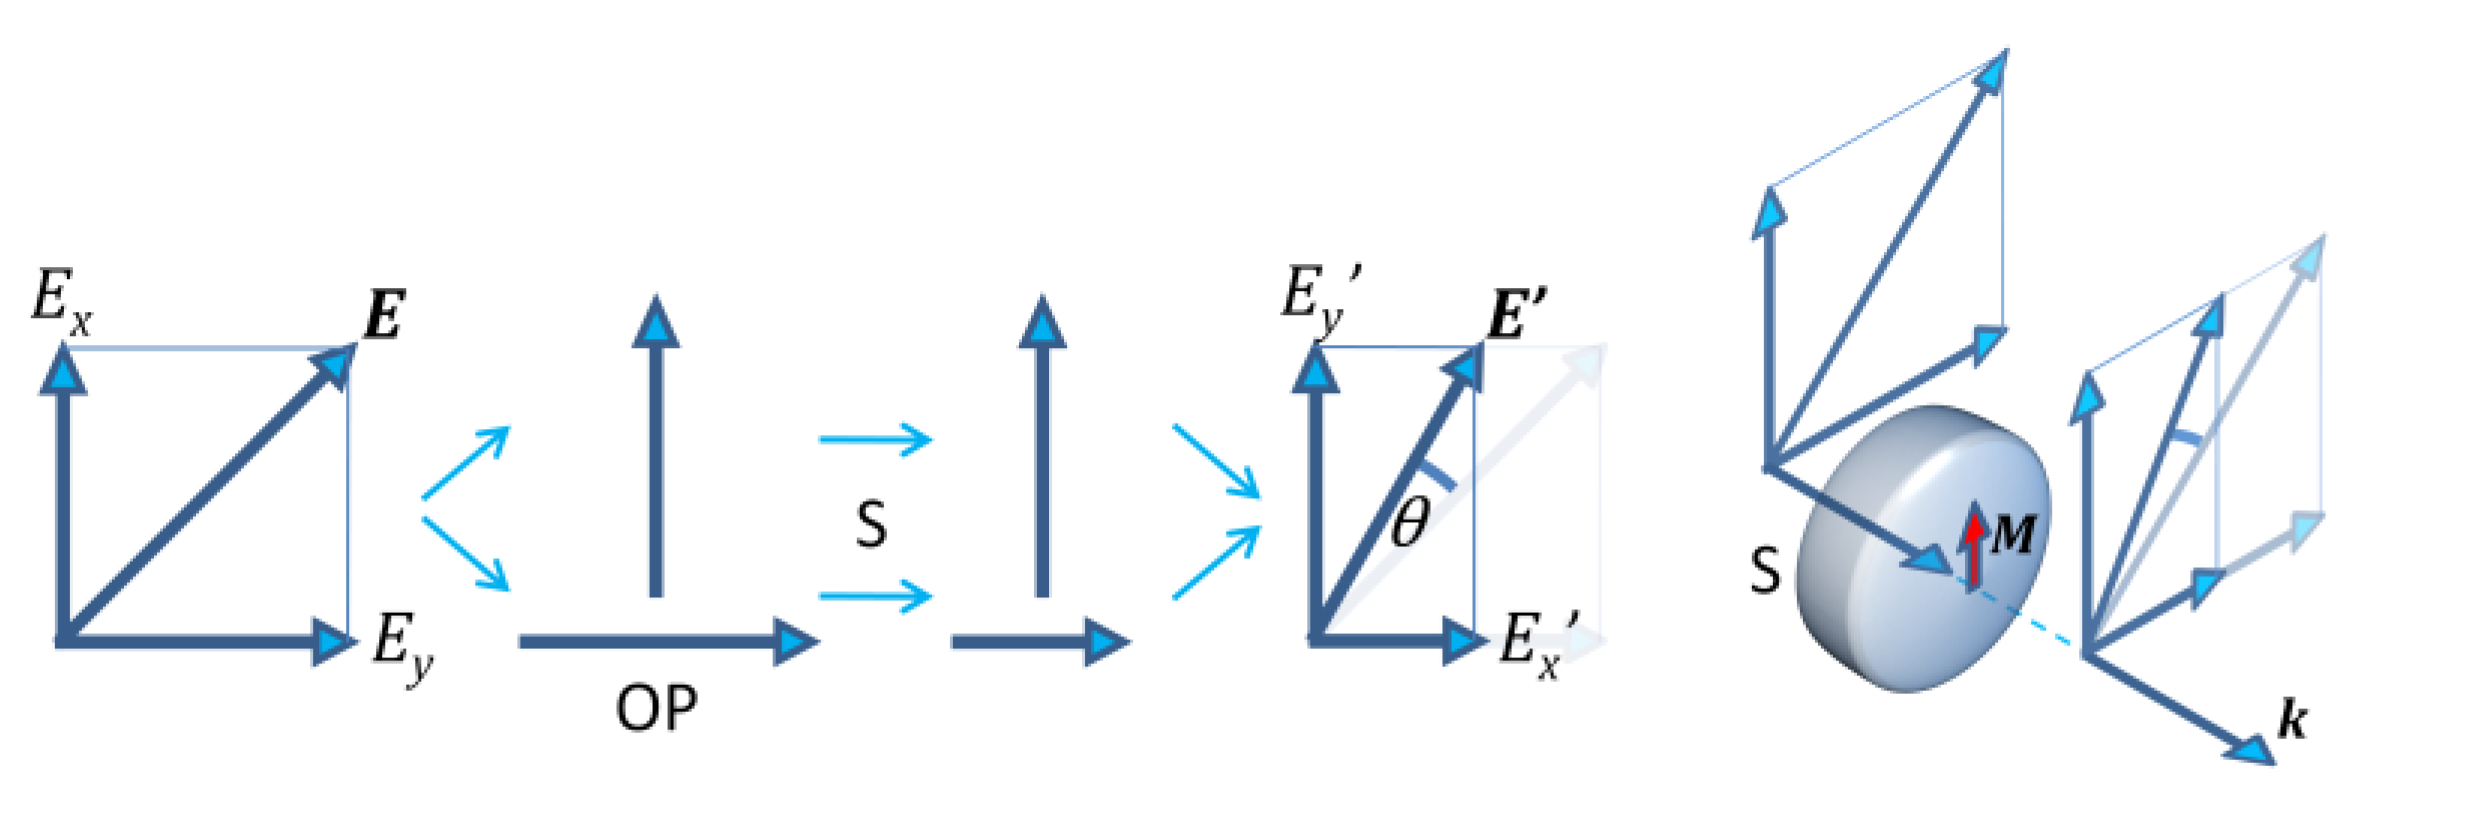
\includegraphics{Subrt_34}}
	\caption{Rotace roviny polarizace vlivem MLD \cite{Subrt}.}\label{mld_subrt}
\end{figure}

V reflexní geometrii se někdy magnetooptické jevy označují jako MOKE (magnetooptical Kerr effect), které se dále rozlišují podle vzájemné orientace vlnového vektoru, roviny vzorku a magnetizace, viz obr.~\ref{kerr_subrt}.

\begin{figure}[htbp]\centering
\qq{	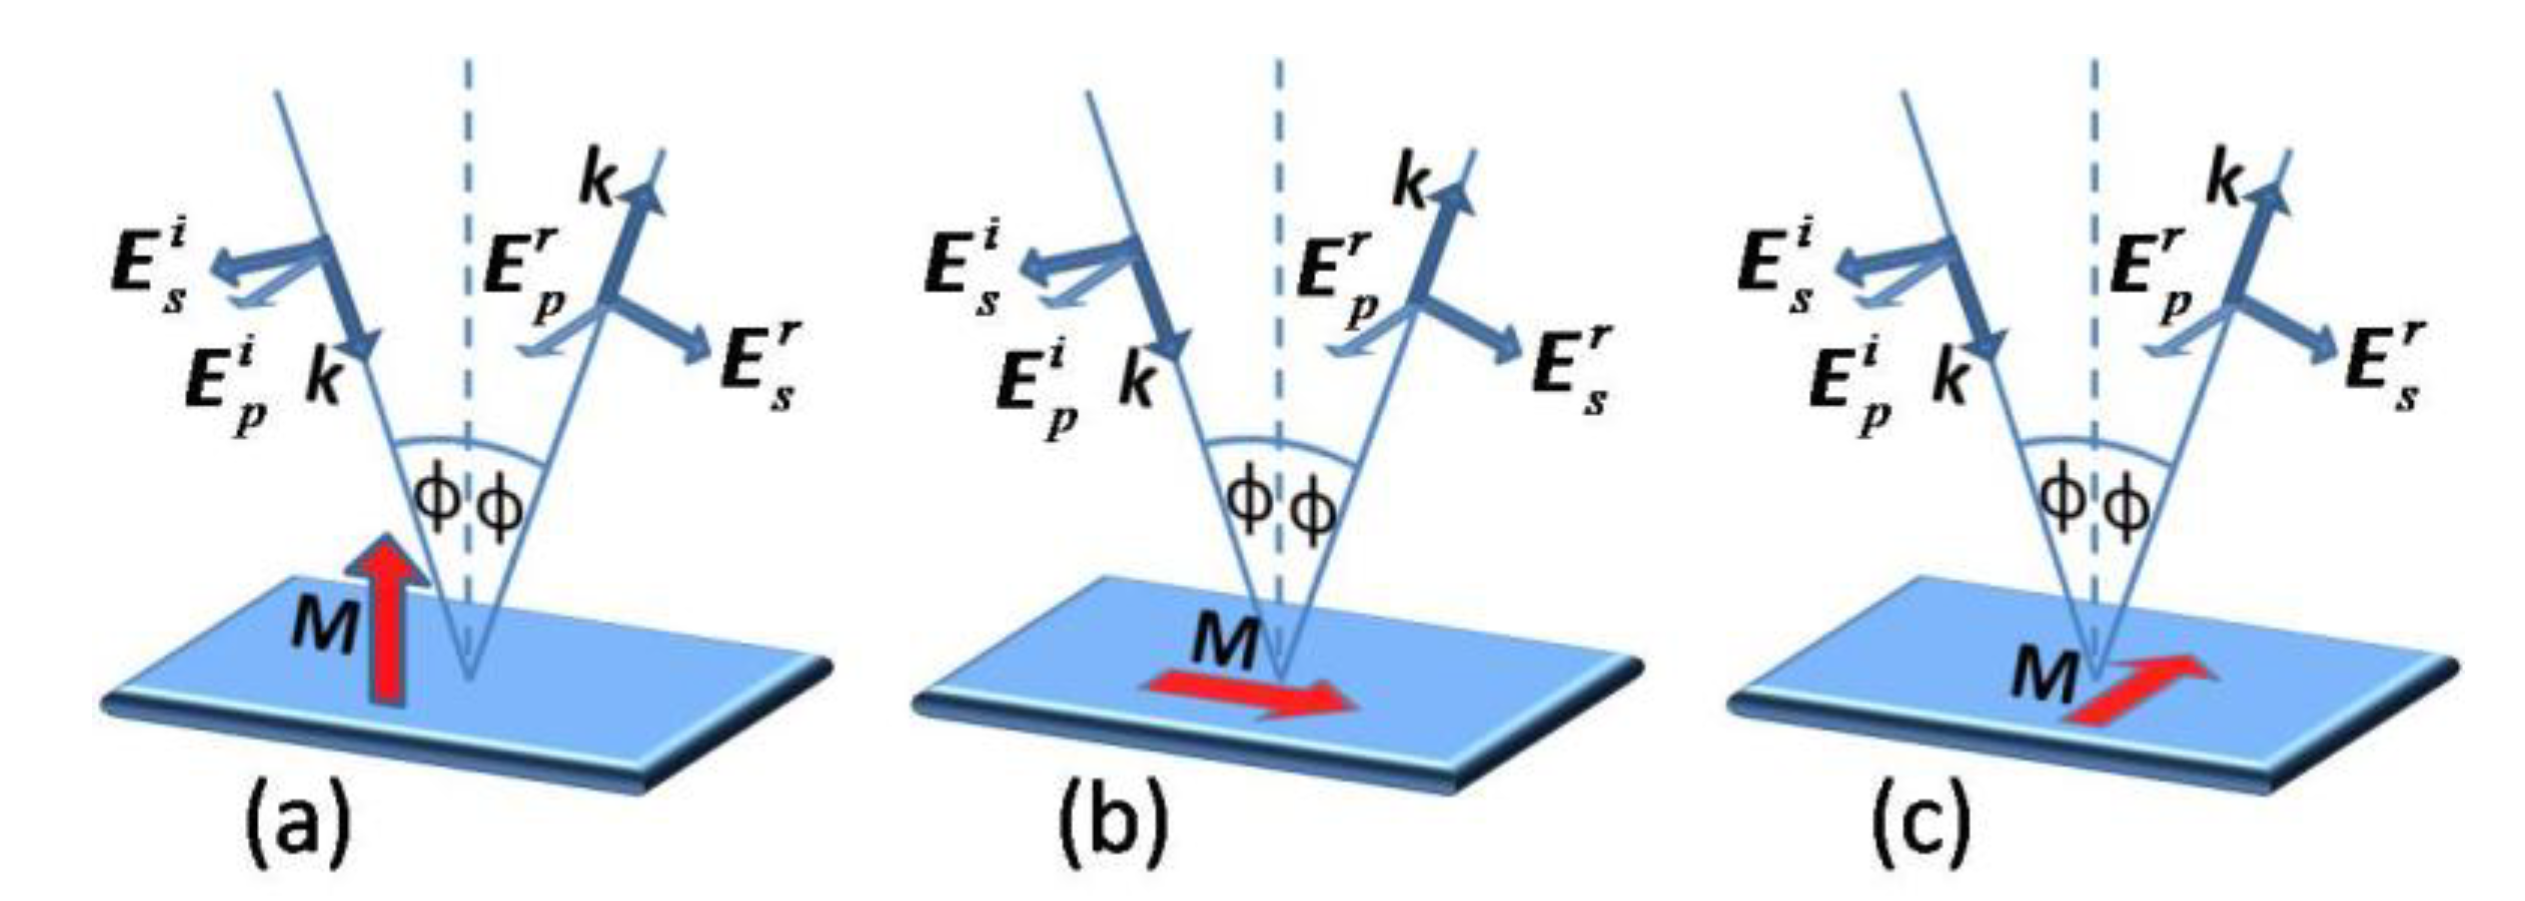
\includegraphics{Subrt_35}}
	\caption{MOKE: (a) polární, (b) longitudinální, (c) transversální \cite{Subrt}.}\label{kerr_subrt}
\end{figure}

\section{Voigtův jev a MLD v reflexní geometrii} \label{kap_VoigtMLD}

MLD je kvadratický (v magnetizaci) magnetooptický jev původně pozorovaný v transmisní geometrii jako dichroismus lineárně polarizovaného světla. Rozdílné absorpční koeficienty pro polarizaci kolmou a rovnoběžnou na směr magnetizace způsobují po průchodu stočení roviny polarizace \cite{cit1}, \cite{cit2}. 

Posléze se jako MLD začal označovat i jiný magnetooptický jev v reflexní geometrii při kolmém a téměř kolmém dopadu \cite{cit3}. Rozdílný reálný index lomu pro obě lineární polarizace způsobuje rozdílnou odrazivost, což má podobně jako u transmisního MLD za následek stočení polarizace. Jev je standardně označován jako MLD, přestože je analogický MLB.

Pro konzistenci s terminologií používanou na našem pracovišti se budeme držet následujícího názvosloví: pokud je studovaný jev rozdílná odrazivost pro lineární polarizaci v různých směrech, jedná se o MLD. Pokud je studovaný jev rotace roviny polarizace, jedná se o Voigtův jev, přestože mají oba jevy původ ve stejné fyzikální skutečnosti. V dalších kapitolách budeme měřit stejné fyzikální veličiny zároveň pomocí MLD i Voigtova jevu a získaná data z obou měření budeme označovat právě tímto způsobem.

MLD signál je v tomto kontextu definován jako \cite{Tesarova}
\begin{equation}
\mld[\si{\radian}]=\frac{1}{2}\frac{I_R^\paral - I_R^\perpen}{I_R^\paral + I_R^\perpen}=\frac{1}{2}\frac{r^2_\paral-r^2_\perpen}{r^2_\paral+r^2_\perpen} \,,
\end{equation}
kde $I_R^\paral$ resp. $I_R^\perpen$ jsou intenzity odraženého světla polarizovaného rovnoběžně resp. kolmo na magnetizaci. Podobně $r_\paral$ a $r_\perpen$ jsou koeficienty reflexe elektrické intenzity (intenzitní odrazivost je rovna $r^2$).

Pokud v rovině vzorku označíme úhel $\phM$ jako směr magnetizace a úhel $\beta$ jako rovinu polarizace\footnote{Soustava souřadná je definovaná v kapitole \ref{exp_usporadani}, vztahy v této kapitole jsou na ní však nezávislé}, pak pro stočení polarizace ($\Delta\beta=\beta^\prime-\beta$) platí \cite{Tesarova} 
\begin{equation}
\tan(\Delta \beta)=\frac{(r_\paral-r_\perpen)\tan(\phM-\beta)}{r_\paral + r_\perpen \tan^2(\phM-\beta)} \,,
\end{equation}
což je pro malé úhly ($r_\paral /r_\perpen \approx 1$)
\begin{equation} \label{rotace_polarizace}
\Delta \beta = \pmld \sin \left[ 2(\phM-\beta) \right] \,,
\end{equation}
kde $\pmld=\num{0.5}(r_\paral/r_\perpen -1)$ je MLD magnetooptický koeficient.

Přestože má situace $\Delta\beta=0$ jasný fyzikální význam (dopadající a odražená polarizace jsou totožné), jsme často schopni určit pouze průběh $\Delta\beta$ až na aditivní konstantu. Dále, zejména v kapitole s experimentálními výsledky, označuje $\Delta\beta$ odchýlení od určitého arbitrárně zvoleného směru.

V přiblížení $r_\paral /r_\perpen \approx 1$ platí
\begin{equation}
\pmld=\frac{1}{2}\frac{r^2_\paral-r^2_\perpen}{r^2_\paral+r^2_\perpen} \,.
\end{equation}

Voigtův jev je tedy polarizačně závislý podle vztahu \eqref{rotace_polarizace} a je největší, když rovina polarizace svírá s magnetizací úhel \ang{45}.

MLD pozorujeme prostřednictvím celkové odražené intenzity $I'$. V příloze \ref{odvozeni_mld} je odvozeno, že v našem přiblížení platí
\begin{equation}
I^\prime=I_0 R \left[1 + 2\pmld \cos[2(\phM-\beta)]\right] \,,
\end{equation}
kde $I_0$ je dopadající intenzita a $R$ je odrazivost vzorku.
Pro studium MLD zavedeme veličinu
\begin{equation} \label{e:Bdef}
B:=\frac{I^\prime}{I_0 R}-1 \,.
\end{equation}

Potom
\begin{equation}
B=2\pmld \cos[2(\phM-\beta)] \,.
\end{equation}
MLD je tedy největší, když porovnáváme odrazivost pro polarizace ve směru rovnoběžném a kolmém na~magnetizaci.
\chapter{GaMnAs}

Všechna magnetooptická měření probíhala s materiálem GaMnAs. GaMnAs je III-V zředěný magnetický polovodič odvozený od polovodiče GaAs, tzn. část atomů Ga byla nahrazena magnetickými atomy Mn, aby materiál získal feromagnetické vlastnosti. Krystalografická struktura Ga$_{1-x}$Mn$_x$As je znázorněna na obr. \ref{gamnasstruktura_reichlova} ($x$ označuje poměr substituovaných Mn atomů).


\begin{figure}[htbp]\centering
\qq{	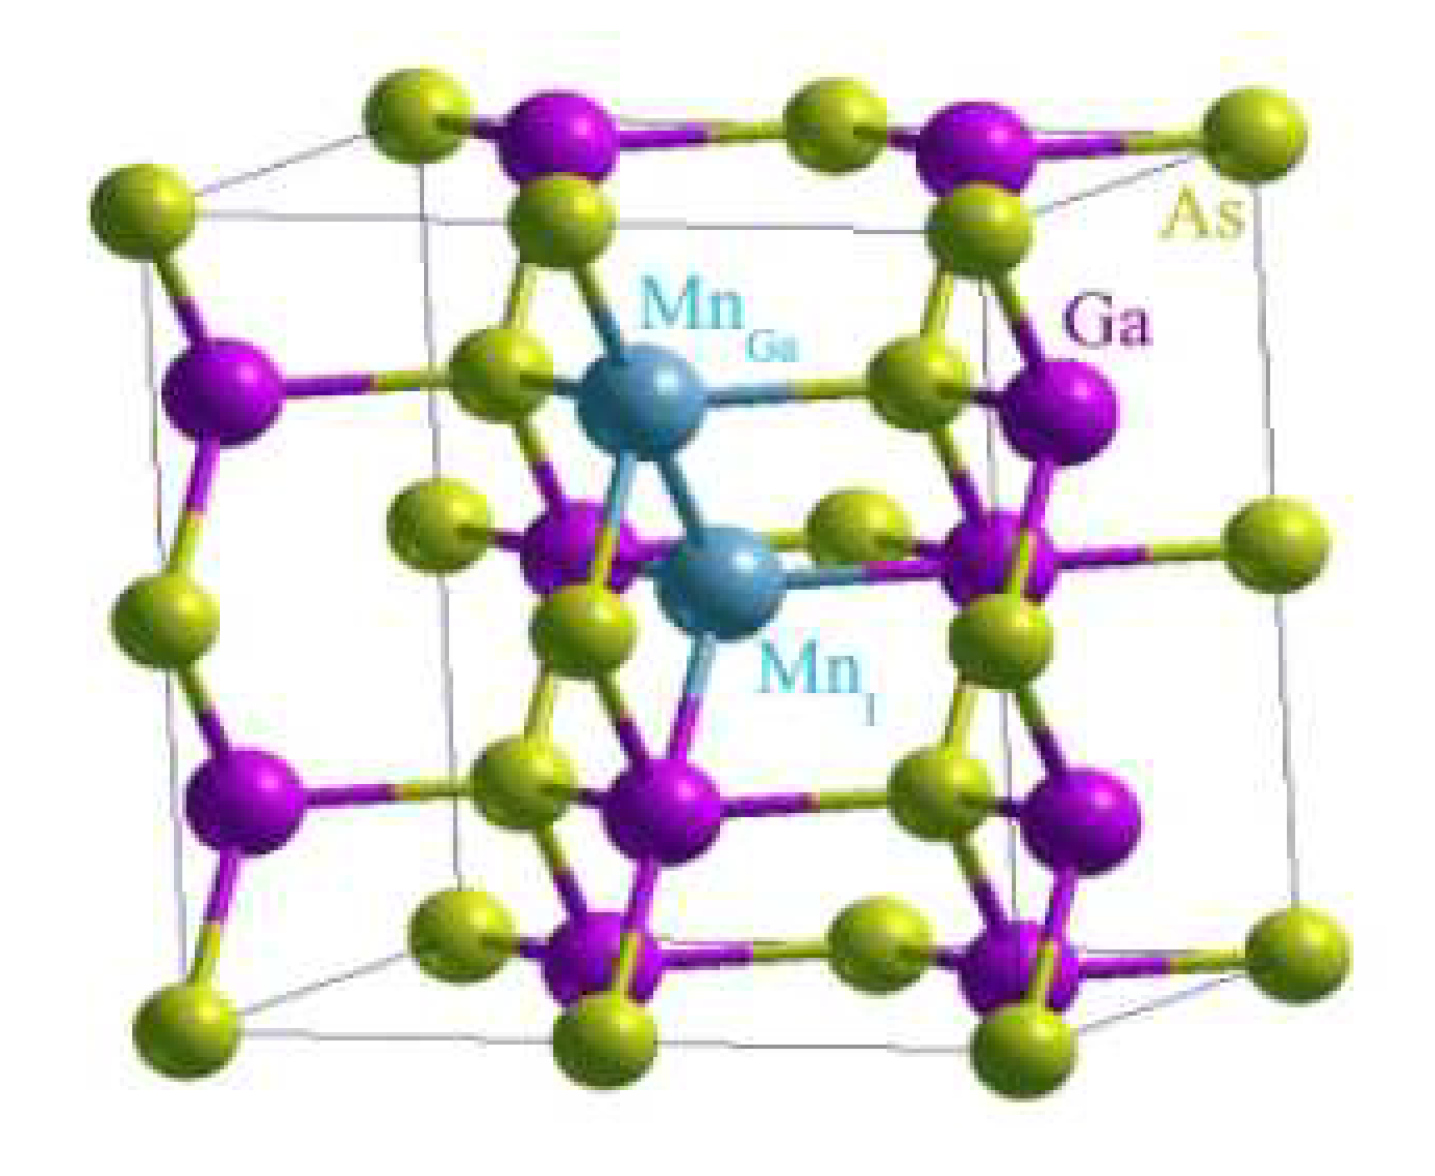
\includegraphics{Reichlova_31}}
	\caption{Krystalografická struktura GaMnAs. Mn$_\text{Ga}$ označuje substituci atomu Ga atomem Mn, Mn$_I$ označuje atom Mn v intersticiální poloze \cite{Reichlova}.}\label{gamnasstruktura_reichlova}
\end{figure}

Feromagnetická interakce mezi lokalizovanými momenty Mn je zprostředkována volnými dírami, a proto feromagnetické vlastnosti GaMnAs silně závisí na~jejich počtu. Vazba Mn-As oproti vazbě Ga-As postrádá jeden elektron. Pokud tedy nahradíme atom Ga atomem Mn, vneseme do krystalu volnou díru. Naopak Mn v intersticiální poloze se stává dvojitým donorem a tím brání vzniku feromagnetismu. Stejně tak atom As substituovaný za Ga se stává dvojitým donorem.

Při přípravě je tedy žádoucí vysoká koncentrace Mn$_\text{Ga}$ a co nejmenší výskyt defektů. 
Vzorky se připravují metodou epitaxe molekulárních svazků za nízké teploty (LT-MBE). Bodové poruchy Mn$_I$ lze poté částečně odstranit žíháním.
Podrobnější popis přípravy vzorků je možno nalézt v \cite{Reichlova}.

\section{Magnetická anizotropie}

V GaMnAs existují v rovině vzorku určité preferované směry magnetizace, tzv. snadné osy. Jejich polohy jsou určeny minimem magnetické energie, která je dána vnějším magnetickým polem, anizotropní energií a výměnnou energií \cite{Reichlova}
\begin{equation}
E=E_\text{pole}+E_\text{anizotropní}+E_\text{výměnná} \,.
\end{equation}

Energie magnetického pole je
\begin{equation}
E_{pole}=-\vec{M}\cdot\vec{H}_\text{ext}
\end{equation}
a má minimum při magnetizaci ve směru vnějšího pole.
Anizotropní energie v sobě zahrnuje příspěvky z kubické anizotropie (minima v krystalografických směrech [100] a [010]) a jednoosé anizotropie (minimum v krystalografickém směru [-110]). 
Výsledkem jsou čtyři snadné osy magnetizace jako na obr. \ref{funkcional_energie} (a).

Na obr. \ref{funkcional_energie} (b) je graf magnetické energie při zapnutém vnějším poli $\hext$. Z obrázku je patrná hysteretická povaha magnetizace, při nižších polích existují lokální minima.

Kubická anizotropie se snižuje s $x$, zatímco jednoosá anizotropie je na $x$ téměř nezávislá \cite{Janda}, což umožňuje připravovat vzorky s různou magnetickou anizotropií.

\begin{figure}[htbp]\centering
\qq{	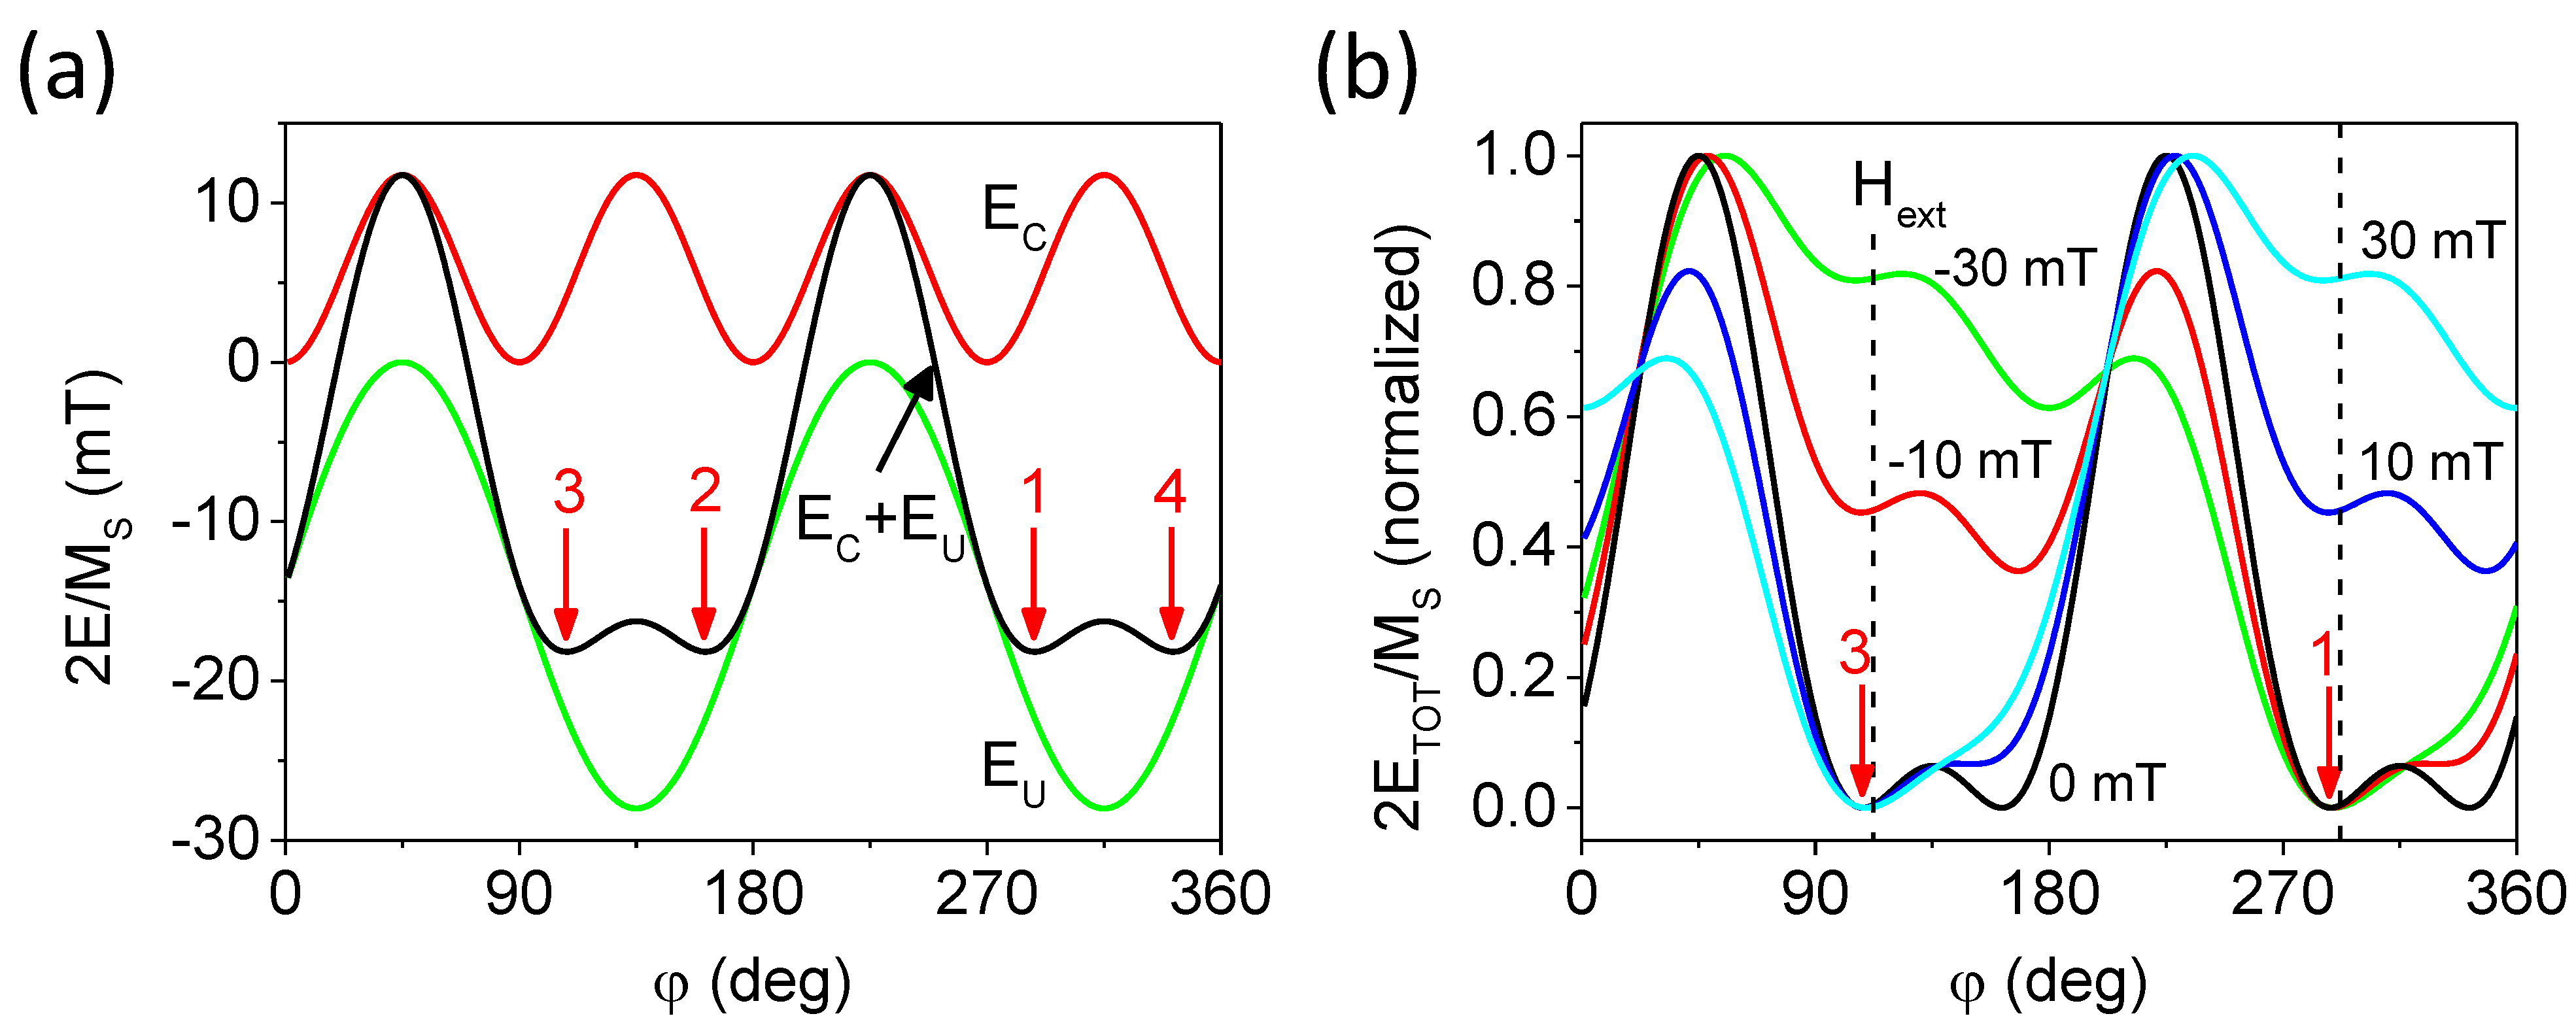
\includegraphics[width=\textwidth]{Voigt_6}}
	\caption{(a) Úhlová závislost kubické ($E_C$), jednoosé ($E_U$) a celkové ($E_C+E_U$) anizotropie ve vzorku Ga$_{1-x}$Mn$_x$As při $x\approx \num{0,038}$. Šipky označují snadné osy magnetizace. 
		(b) Stejný vzorek po přiložení vnějšího pole $H_\text{ext}$ ve směru přerušované čáry (\ang{112}) pro kladné i záporné pole \cite{Janda}.}\label{funkcional_energie}
\end{figure}

\section{Vzorek F002} \label{kap_vzorek}

V této práci byl měřen jediný vzorek označený F002. Vzorek byl vybrán proto, že už na něm podobná měření byla v minulosti provedena, viz \cite{Reichlova}. Byl připravený metodou LT-MBE ve Fyzikálním ústavu Akademie věd v Cukrovarné ulici. Základní vlastnosti vzorku shrnuje tabulka \ref{tab_vzorek}. Na obr. \ref{charakterizace_vzorku} je charakterizace vzorku pomocí SQUID magnetometru.

\begin{table}[htbp]	
	\centering	
	\begin{tabular}{c|c}
		koncentrace Mn & \SI{3}{\percent} \\ \hline
		tloušťka & \SI{20}{\nano\metre} \\ \hline
		Curieova teplota & \SI{75}{\kelvin} \\ \hline
		snadné osy & \ang{104}, \ang{166}, \ang{284}, \ang{346} \\
		magnetizace & $\pm$ \ang{5}
	\end{tabular}
	\caption{Charakterizace měřeného vzorku F002 \cite{Reichlova}, \cite{TesarovaDisertace}. Úhly jsou měřené od~krystalografického směru [100] k [010], viz níže obr. \ref{souradna_soustava_vzorek} (b).}
	\label{tab_vzorek}
\end{table}


\begin{figure}[htbp]\centering
	\qq{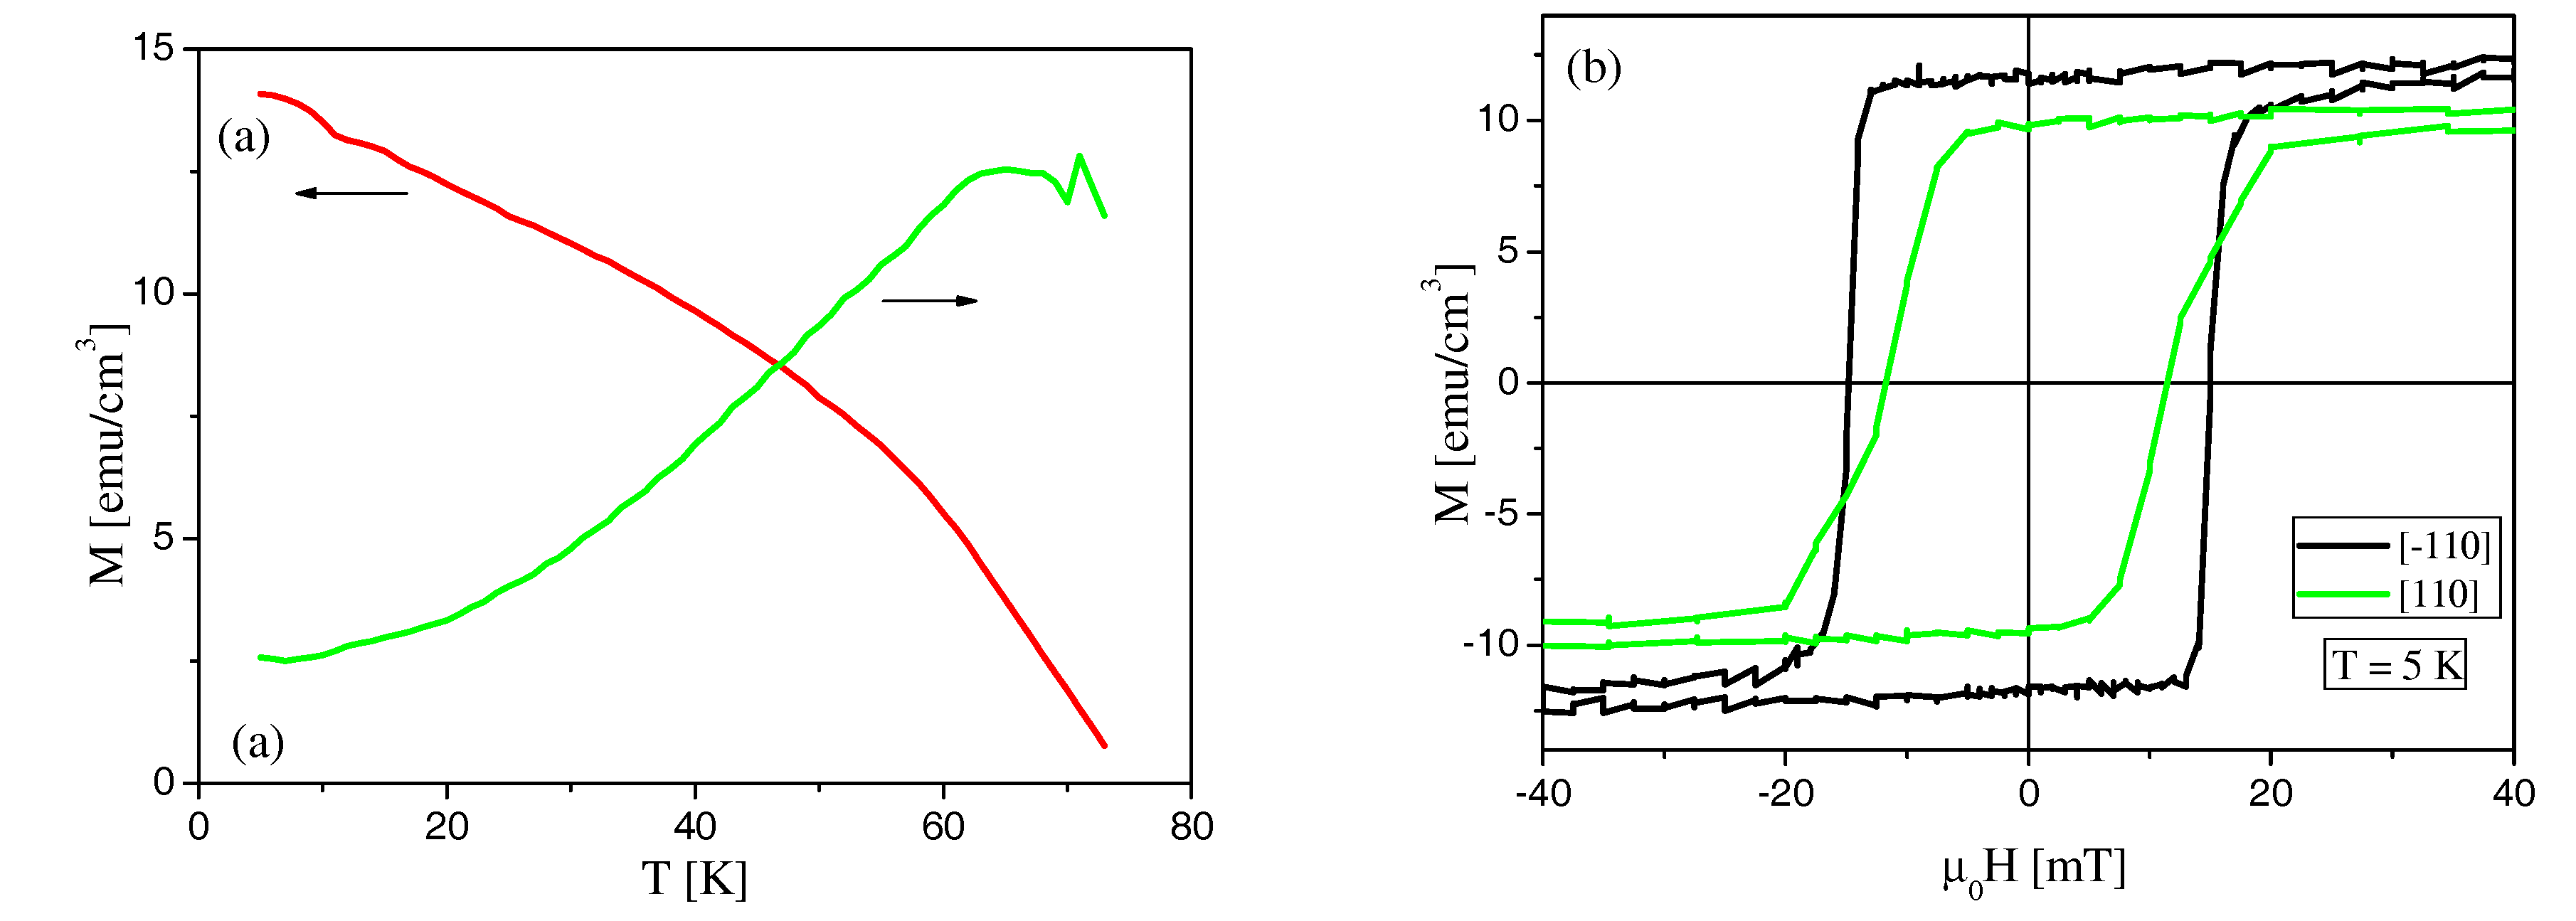
\includegraphics[width=\textwidth]{Reichlova_61}}
	\caption{Charakterizace vzorku pomocí SQUID magnetometru. (a) Závislost magnetizace na teplotě (červená křivka). (b) Závislost magnetizace na velikosti přiloženého magnetického pole pro dva různé směry pole \cite{Reichlova}.}\label{charakterizace_vzorku}
\end{figure}

\section{Studium hysterezních smyček pomocí Voigtova jevu a MLD}

Díky přítomnosti snadných os dochází při plynulé změně vnějšího pole k přeskokům magnetizace. Představme si následující experiment.
Vzorek je umístěn v~elektromagnetu jako na obr. \ref{revsci_mld} (c).


Při vysokém záporném poli $H_\text{ext}$ je magnetizace ve směru blízkém M$_3$. Pokud budeme záporné pole snižovat a poté zvyšovat do kladných hodnot, při určitém $H_\text{ext}=\hcj$ dojde k~přeskoku do snadné osy M$_4$. Po dalším zvyšování pole dojde při $H_\text{ext}=\hcd$ k přeskoku do M$_1$, kde zůstane. Pokud budeme poté pole snižovat zpět do záporných hodnot, situace bude podobná, při $H_\text{ext}=-\hcj$ dojde k přeskoku do M$_2$ a při $H_\text{ext}=-\hcd$ k~přeskoku do M$_3$.

Pokud při takovém procesu budeme měřit stočení roviny polarizace, dostaneme vzhledem k sudosti Voigtova jevu výsledky jako na obr. \ref{revsci_mld} (a), v osách M$_1$ a M$_3$ je signál stejný, v M$_2$ a M$_4$ také.
Hysterezní smyčka je charakterizována amplitudou $A$ a dvěma hysterezními poli $\hcj$ a $\hcd$ jako na obr. \ref{charakterizace_hystereznismycky}.

Amplituda Voigtova jevu $A$ v uvedené hysterezní smyčce je dána $A=\Delta \beta_4 - \Delta \beta_1$, která je při zavedení úhlů jako v obr. \ref{revsci_mld} (d) rovna \cite{Tesarova}
\begin{equation} \label{e:amplVoigt}
A =2 \pmld \cos\left[2(\gamma-\beta)\right] \sin(\xi)
\end{equation}
a tedy její polarizační závislost je jako na obr. \ref{revsci_mld} (b). Vztah je odvozen v \cite{Reichlova}.

U MLD je situace podobná (odvození v příloze 1).
Při přeskoku dojde ke~změně signálu $B$: $\Delta B=B_4-B_1$
\begin{equation} \label{e:amplMLD}
\Delta B=-4\pmld  \sin[2(\gamma-\beta)]\sin(\xi) \,.
\end{equation}

V případě, že v hysterezní smyčce je na začátku magnetizace v ose M$_2$ nebo M$_4$ a přeskok probíhá přes M$_1$ nebo M$_3$, pak má amplituda přeskoku opačné znaménko, tj. $A=\Delta \beta_1 - \Delta \beta_4$ a $\Delta B=B_1-B_4$. Vztahy \eqref{e:amplVoigt} a \eqref{e:amplMLD} pak mají opačné znaménko. Veličiny $A$ a $\Delta B$ definujeme vždy tak, aby odpovídaly výšce \uv{hrbu} oproti pozadí.

\begin{figure}[htbp]\centering
\qq{	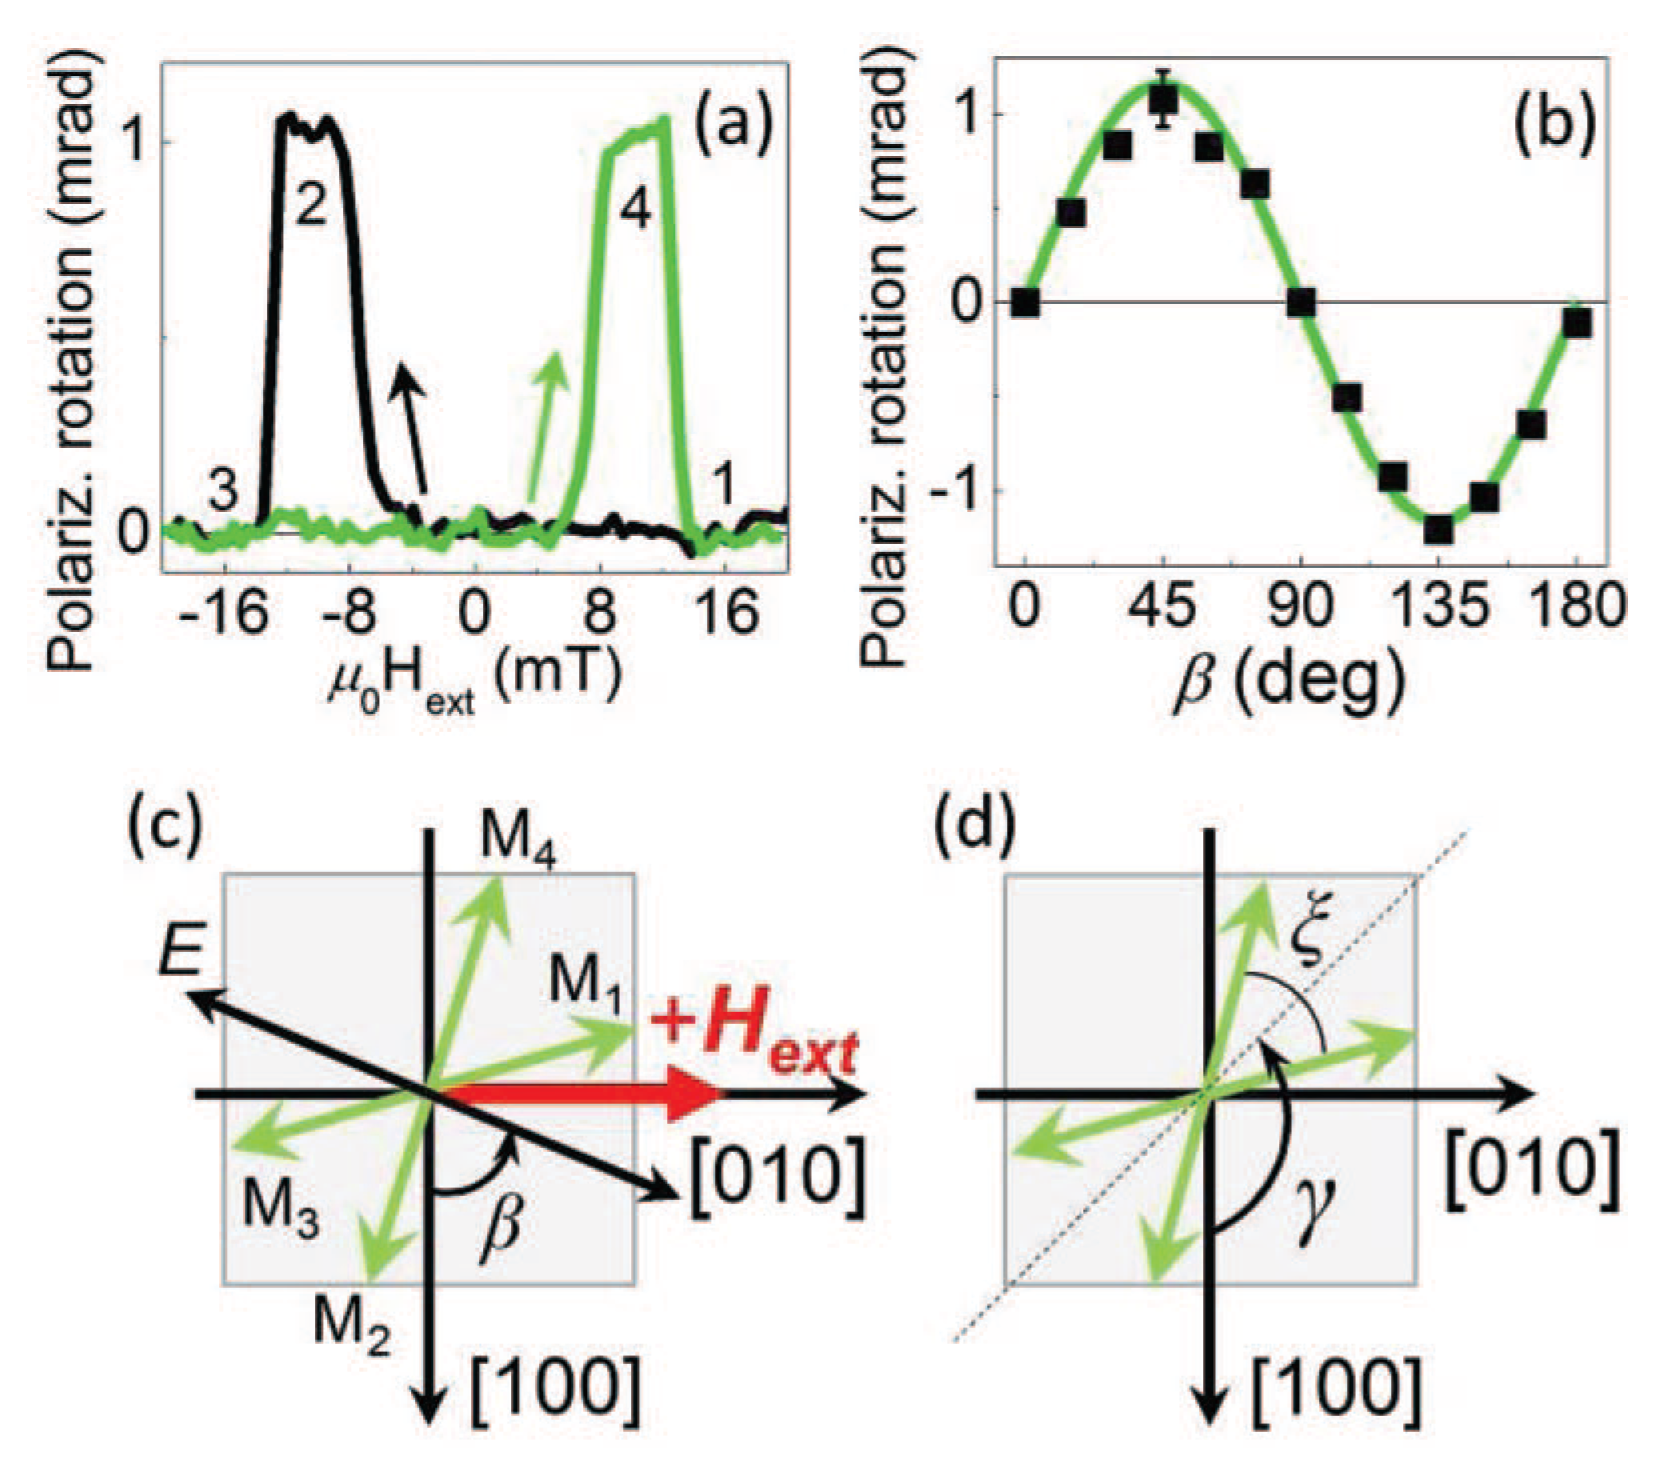
\includegraphics[width=0.7\textwidth]{revsci_4}}
	\caption{(a) Voigtův jev při průchodu hysterezní smyčkou. Šipky naznačují směr změny pole a čísla označují, do které snadné osy mířila magnetizace. (b) Polarizační závislost amplitudy hysterezní smyčky.
		(c) Umístění vzorku v elektromagnetu. M$_1$-M$_4$ jsou snadné osy, vnější pole $H_\text{ext}$ v tomto případě přikládáme ve směru [010], dopadající světlo je lineárně polarizované pod úhlem $\beta$. (d) Definice úhlů. $\gamma$ je směr bisektrisy snadných os, $\xi$ je úhel, který svírají dvě přilehlé snadné osy \cite{Tesarova}. Soustava souřadná je definovaná v kapitole \ref{exp_usporadani}.}\label{revsci_mld}
\end{figure}

\begin{figure}[htbp]\centering
	\qq{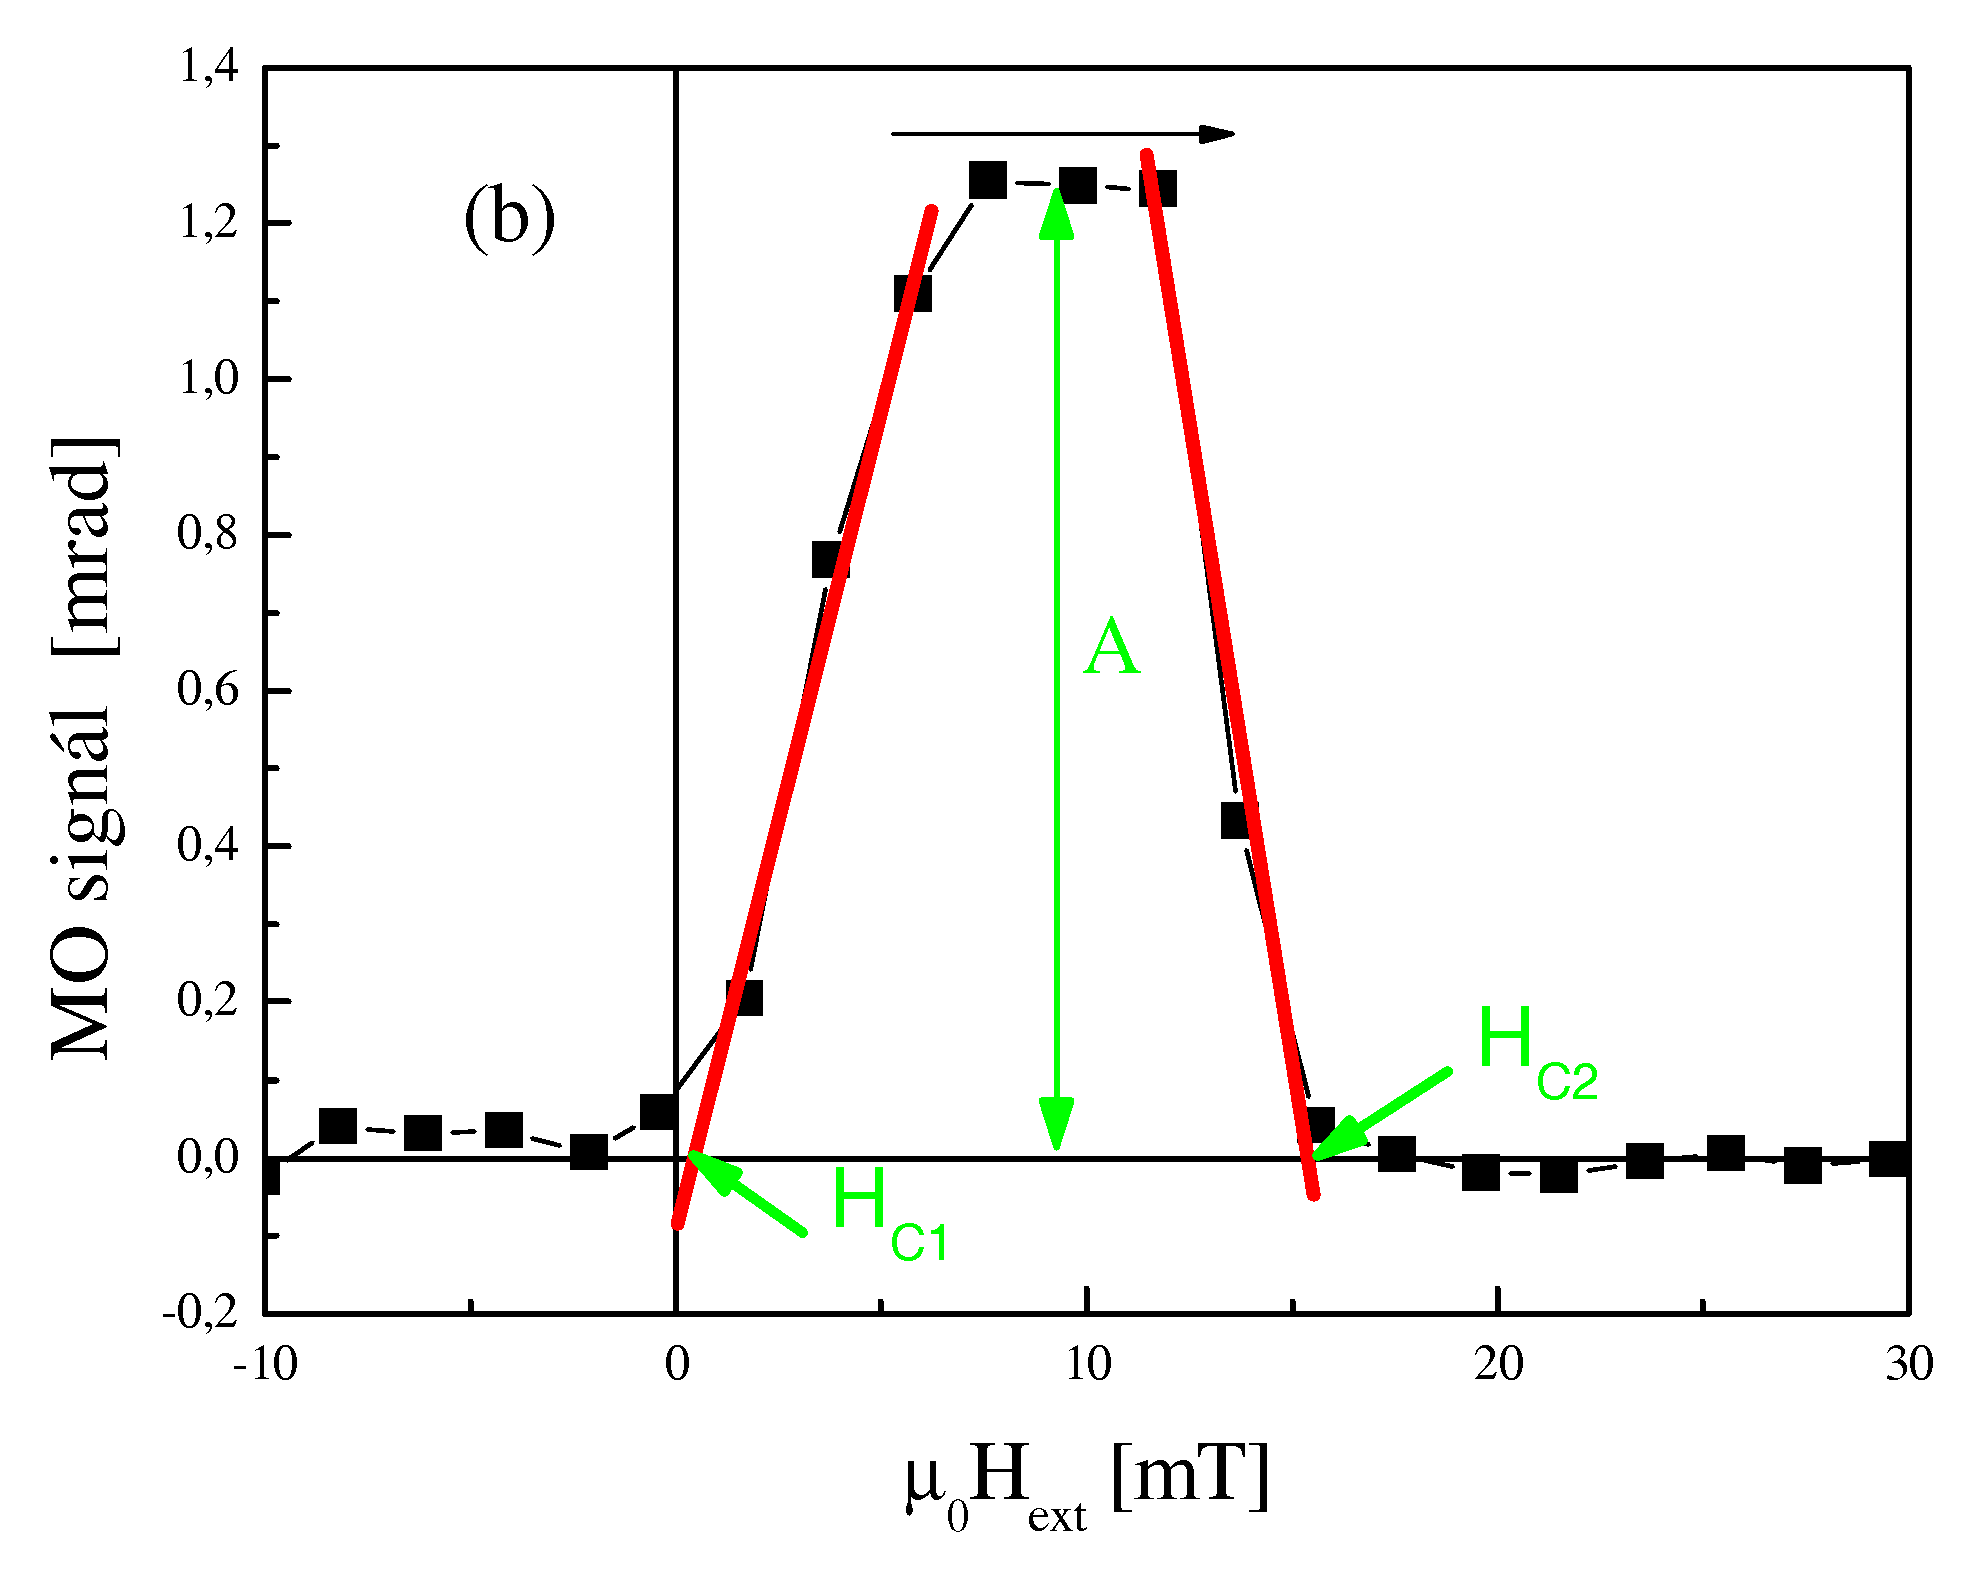
\includegraphics[width=0.5\textwidth]{Reichlova_101b}}
	\caption{Typická hysterezní smyčka (pouze up) a význam veličin $A$, $\hcj$ a $\hcd$ \cite{Reichlova}.}\label{charakterizace_hystereznismycky}
\end{figure}

V práci \cite{Reichlova} bylo změřené MLD vzorku F002 při teplotě \SI{15}{\kelvin} statickou metodou, přímo měřením polarizační závislosti intenzitní odrazivosti 
\begin{equation}
\pmld=\SI{-0,9(1)}{\milli\radian} \,.
\end{equation}

Podle měření provedených v práci \cite{Reichlova} jsou magnetické vlastnosti vzorku vysoce závislé na teplotě. S rostoucí teplotou dochází ke snižování koercitivních polí a koeficientu $\pmld$.
\chapter{Experimentální uspořádání} \label{exp_usporadani}
Jediný vzorek, který byl v rámci této práce studován, je vzorek GaMnAs s~označením F002, který je popsán v kapitole \ref{kap_vzorek}.

Použili jsme laser Thorlabs LDM785 s vlnovou délkou $\lambda=\SI{785}{\nm}$.

Všechna měření jsme prováděli v jedné ze dvou geometrií. V nekolineární geometrii, ve které laserový svazek nedopadá přímo kolmo na vzorek a odražený svazek je tedy vychýlený a dobře oddělený od vstupujícího svazku, jsme provedli měření hysterezních smyček. Stejná měření na stejném vzorku byla již provedena v práci \cite{Reichlova}. Cílem tohoto měření bylo ověření funkčnosti setupu.

Poté jsme přešli do kolineární geometrie (kolmý dopad na vzorek). V ní je vzorek i magnetické pole v rovině kolmé na směr šíření svazku. V této geometrii jsme provedli všechna zbývající měření.


\subsubsection*{Soustava souřadná}
Osu $z$ ztotožňujeme s osou elektromagnetu a chodem paprsku před dopadem na vzorek. Laser tedy svítí ve směru vektoru $-\vec{z}$.
Osa $x$ míří dolů a osa $y$ při pohledu ve směru svazku doprava ($xyz$ tvoří pravotočivou soustavu). Viz obr. \ref{souradna_soustava_vzorek}.

Elektromagnet dokáže při tomto označení generovat magnetické pole $\vec{H}_{\text{ext}}$ v~rovině $xy$.

Všechny úhly v rovině $xy$ (vnější pole $\phH$, magnetizace $\phM$, rovina polarizace $\beta$, bisektrisa snadných os $\gamma$, úhel mezi snadnými osami $\xi$) měříme od osy $x$ směrem k ose $y$. $\vec{x}$ je tedy ve směru \ang{0} a  $\vec{y}$ ve směru \ang{90}.


Podle \cite{TesarovaDisertace} mají být snadné osy vzorku v našem uspořádání ve směrech \ang{59}, \ang{121}, \ang{239}, \ang{301} ($\pm$~\ang{5}). Bisektrisa dvou přilehlých snadných os je ve směru $\gamma=\ang{90}$.


\begin{figure}[htbp]\centering
	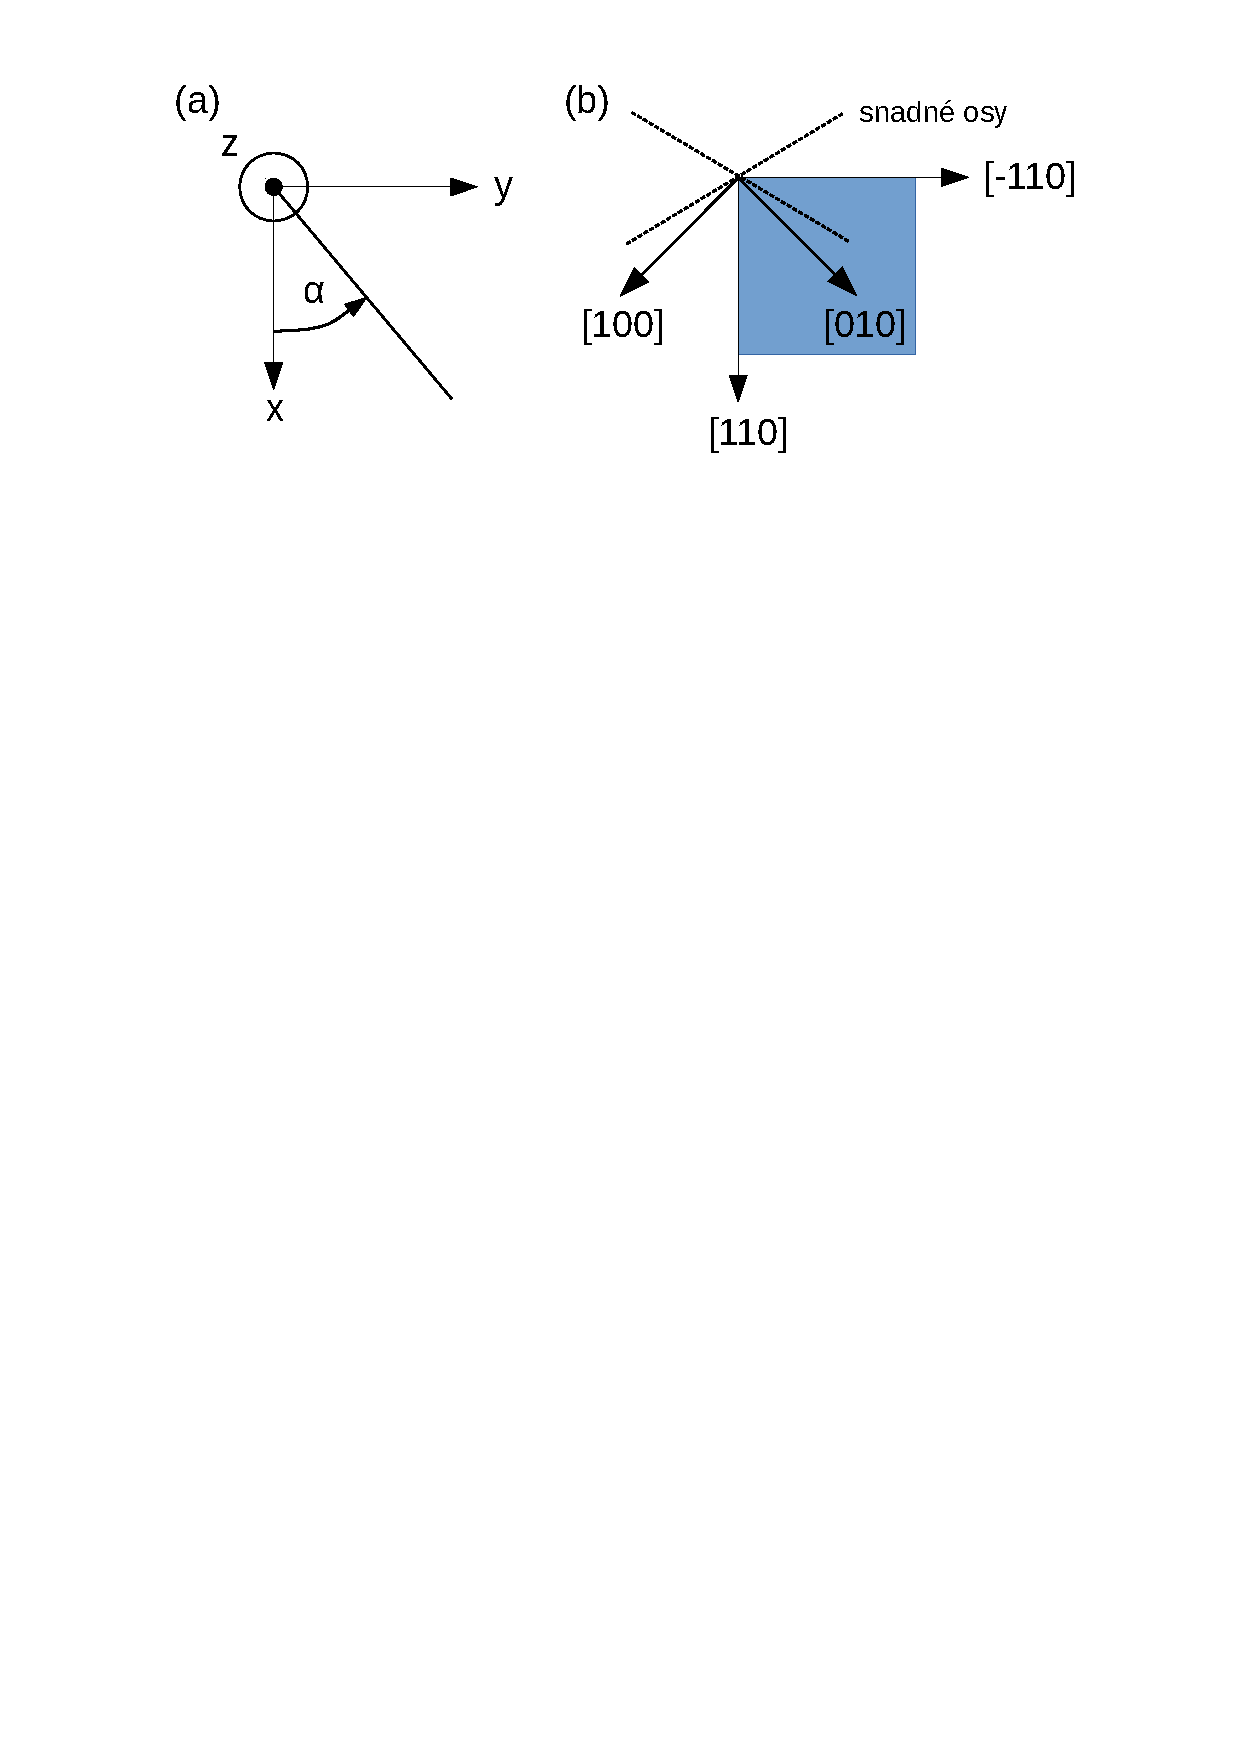
\includegraphics[trim={1in 8.5in 1in 0.5in}, clip, width=\textwidth]{./png/soustava}
	\caption{(a) Zavedení soustavy souřadné. Pohled ve směru chodu paprsku dopadajícího na vzorek. (b) Umístění vzorku na studeném prstu kryostatu.}\label{souradna_soustava_vzorek}
\end{figure}


\subsubsection*{Nekolineární geometrie}

Schéma experimentálního uspořádání v nekolineární geometrii je na obr. \ref{nekolinearni_usporadani}.

Po výstupu z laseru svazek nejprve prochází modulátorem intenzity (přerušovač svazku).
Svazek dále prochází dvěma polarizátory s osou ve směru \ang{0}, mezi kterými je umístěna $\lambda/2$ fázová destička kvůli nastavení intenzity vystupujícího světla. Vystupující polarizace je lineární $\beta=\ang{0}$.

Následuje $\lambda/2$ fázová destička, pomocí které nastavujeme rovinu polarizace $\beta$ světla dopadajícího na svazek. Svazek je dále fokusován \SI{5}{D} spojnou čočkou na vzorek, který je umístěn mezi pólovými nástavci magnetu. 

Vzorek mírně vykloněn z roviny $xy$, takže se odražený svazek odchyluje od dopadajícího. Úhel mezi dopadajícím a odraženým svazkem je $\ang{6,6}\pm\ang{0,5}$, úhel dopadu na vzorek je tedy $\ang{3,3}\pm\ang{0,3}$.
Odražený svazek koliminujeme další \SI{5}{D} spojnou čočkou.

Zbývající část uspořádání se označuje jako \emph{optický můstek}. Podrobný popis lze nalézt např. v \cite{Rozkotova}. Hlavní komponentou můstku je polarizátor, který svazek rozdělí na svislou a vodorovnou polarizaci. Před můstkem je umístěna vyvažovací $\lambda/2$ fázová destička s piezo ovládáním, pomocí které otáčíme rovinu polarizace tak, aby intenzita v obou ramenech byla stejná. Oba svazky dále fokusujeme do detektorů.
Detektory jsou připojené na dva elektronické směšovače, které signály z obou detektorů sečtou (A+B) a odečtou (A-B). Oba směšovače jsou připojené do fázově citlivých zesilovačů (\emph{lock-in}).
Hlavní výhodou optického můstku je, že měříme přímo rozdílový signál a vyhneme se tím odčítání blízkých čísel. Navíc fluktuace v intenzitě laseru se rovnoměrně rozdělí do obou ramen a odečtou se.

Z lock-inů dostáváme dva signály $I_{A+B}$ a $I_{A-B}$. Pokud při určitém polarizačním stavu světla vyvážíme můstek a následně dojde ke stočení roviny polarizace, dojde také k rozvážení můstku. Pro malé úhly ho můžeme určit jako \cite{Rozkotova}
\begin{equation} \label{e:mustek}
\beta = \pm\frac{I_{A-B}}{2I_{A+B}} \,,
\end{equation}
kde znaménko $+$, nebo $-$ závisí na tom, v jaké ze dvou vyvažujících poloh je vyvažovací $\lambda/2$ destička, a který z detektorů detekuje jakou polarizaci. My jsme znaménko určili z měření v kapitole \ref{kap_toceni}. Stejný jev měříme pomocí Voigtova jevu (z~rozdílového signálu) a MLD (ze součtového signálu). MLD nám dovoluje jednoduše určit znaménko jevu, a protože Voigtův jev by měl dát tu samou informaci, tak určíme správné znaménko.

Použité směšovače nejsou totožné a při stejném zesílení se jejich výstupní napětí liší až o \SI{5}{\percent}, ale korekci na tuto skutečnost neprovádíme.

\begin{figure}[htbp]\centering
	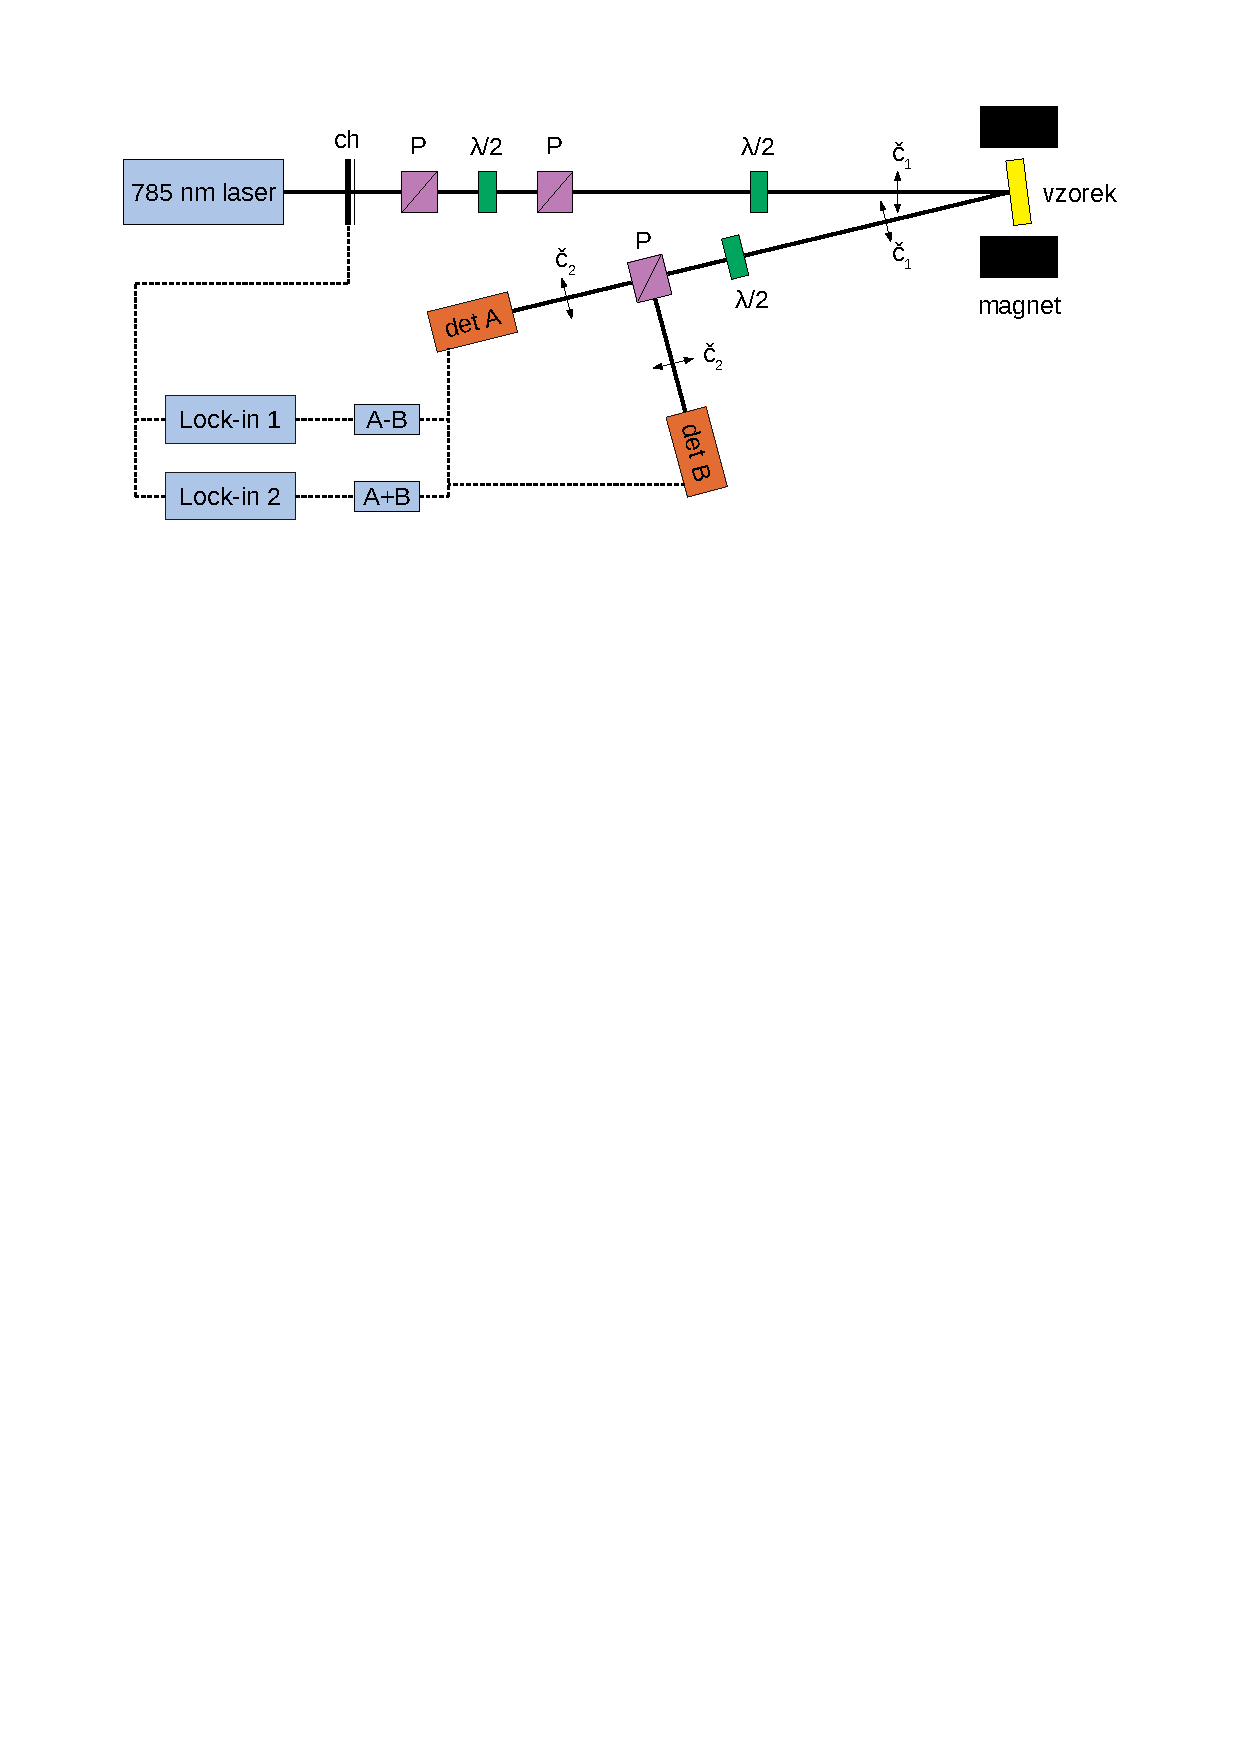
\includegraphics[trim={0,7in 8in 0,7in 0.5in}, clip, width=\textwidth]{./png/nekolinearni_usporadani}
	\caption{Experimentální uspořádání v nekolineární geometrii. ch --- přerušovač svazku, P --- polarizátor, $\lambda/2$ --- půlvlnná destička, č$_\text{i}$ --- spojná čočka.}\label{nekolinearni_usporadani}
\end{figure}

\FloatBarrier

\subsubsection*{Kolineární geometrie}
Schéma experimentálního uspořádání v kolineární geometrii je na obr. \ref{kolinearni_usporadani}.

První část uspořádání je stejná. Vzorek je však nyní kolmo na dopadající svazek a ten se tedy vrací stejnou drahou zpět (odtud označení \emph{kolineární}). Odražený svazek je opět koliminován spojnou čočkou a projde zpět $\lambda/2$ destičkou. Za ní je umístěn dělič svazku, který nám umožní od sebe oddělit oba svazky šířící se proti sobě.
Děličem odražený svazek detekujeme opět pomocí optického můstku.

V kolineární geometrii se nám na rozdíl od nekolineární geometrie nepodařilo oddělit od sebe svazek odražený od vzorku a svazek odražený od okénka kryostatu. Následkem toho v můstku detekujeme navíc světlo, které nenese žádnou informaci o vzorku a je nezávislé na vnějším magnetickém poli. Vztahy použité pro korekci jsou uvedeny a odvozeny v přiloze \ref{odvozeni_kolinearni}.


\begin{figure}[htbp]\centering
	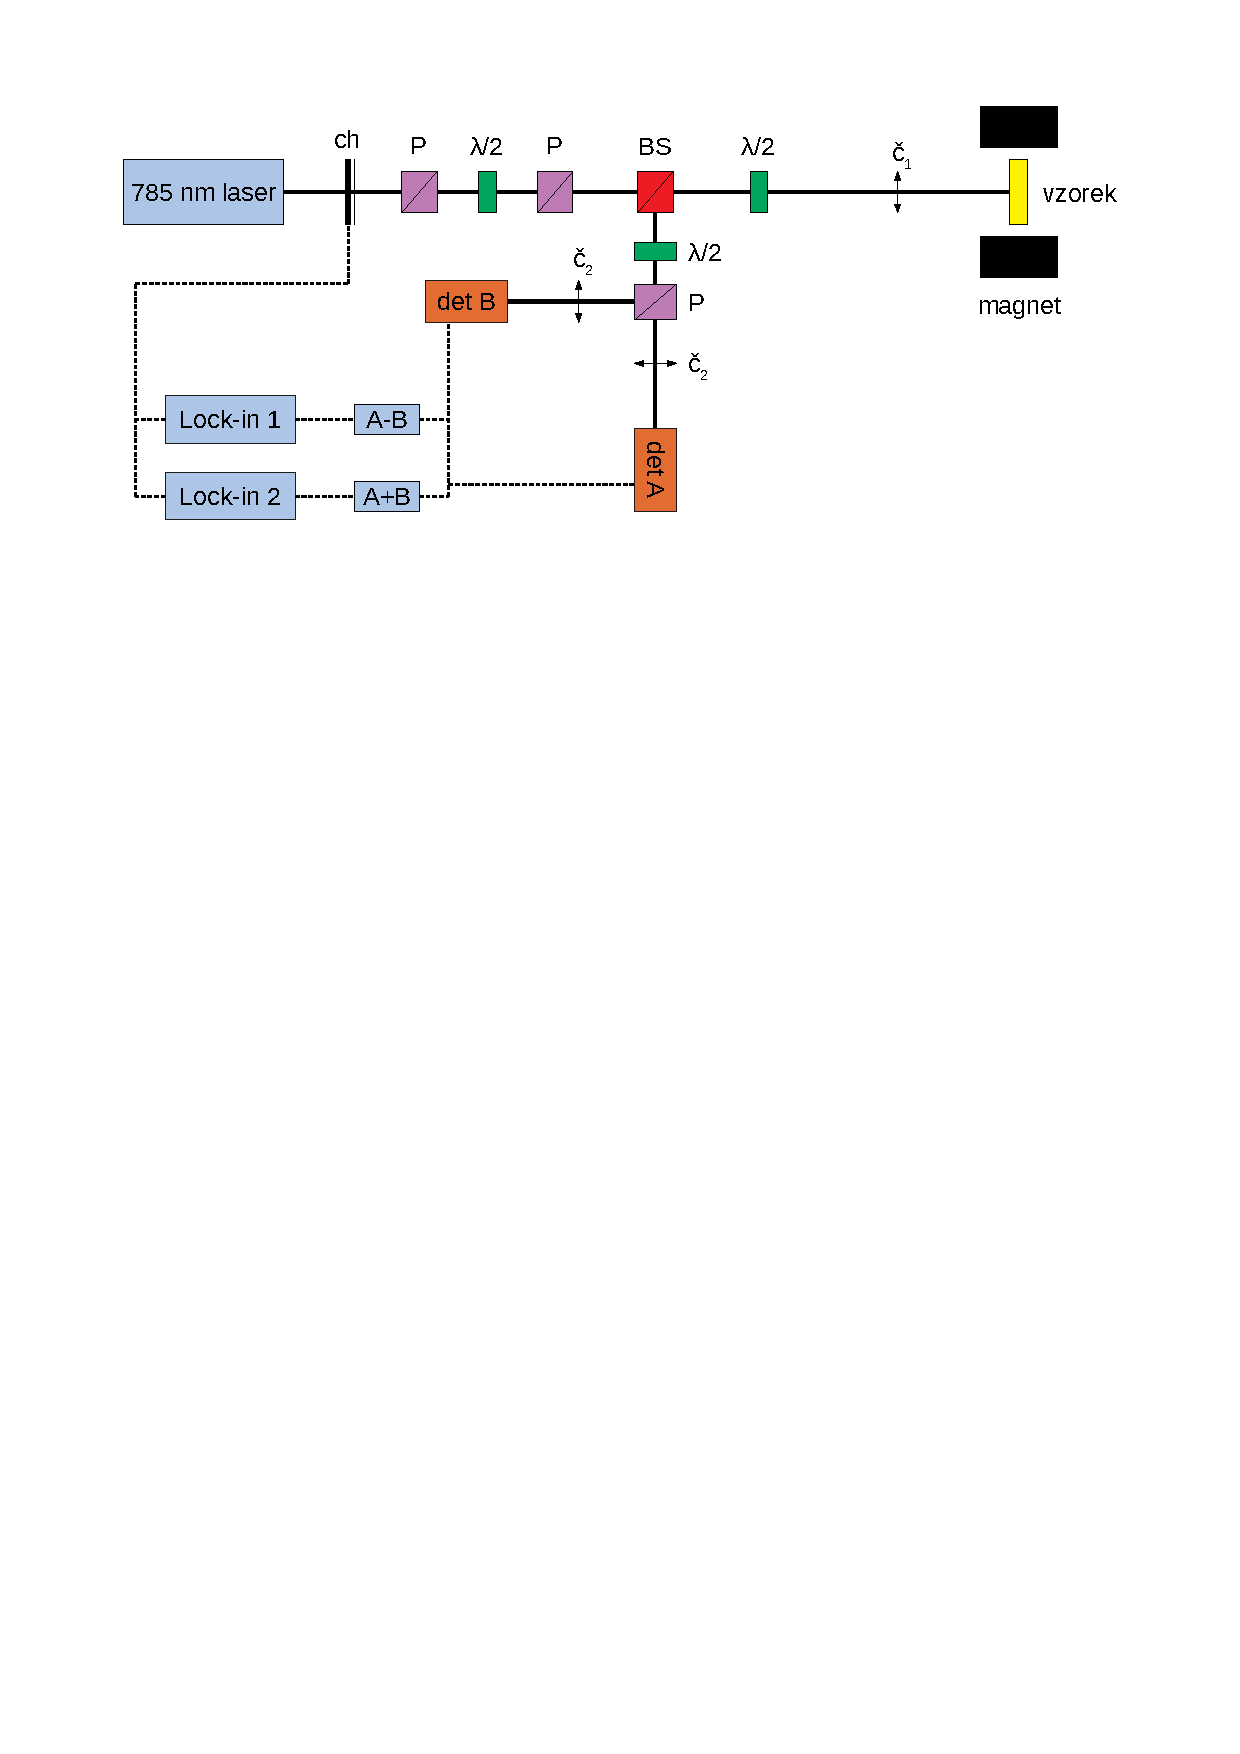
\includegraphics[trim={0,7in 8in 0,7in 0.5in}, clip, width=\textwidth]{./png/kolinearni_usporadani}
	\caption{Experimentální uspořádání v kolineární geometrii. ch --- přerušovač svazku, P --- polarizátor, $\lambda/2$ --- půlvlnná destička, č$_\text{i}$ --- spojná čočka, BS --- dělič svazku.}\label{kolinearni_usporadani}
\end{figure}

\FloatBarrier

\subsubsection*{Kryostat}

Protože GaMnAs má feromagnetické vlastnosti pouze za nízkých teplot, je do středu elektromagnetu zavedeno rameno kryostatu, který umožňuje nastavení teplot v rozmezí cca 5 až \SI{800}{\kelvin}. Vzorek je umístěn na tzv. studeném prstu (\emph{cold finger}) kryostatu. Kryostat je dále opatřen skleněnými okénky pro průchod světla. V~kryostatu jsou umístěny celkem tři teplotní čidla, křemíková dioda, platinové čidlo a termočlánek. Křemíková dioda je umístěná přibližně v půlce ramene kryostatu, zatímco platinové čidlo a termočlánek jsou blízko vzorku.
Při všech měřeních jsme zaznamenali teplotu všech čidel a určili skutečnou teplotu z dříve provedené kalibrace, viz obr. \ref{sensor}.

\begin{figure}[htbp]\centering
	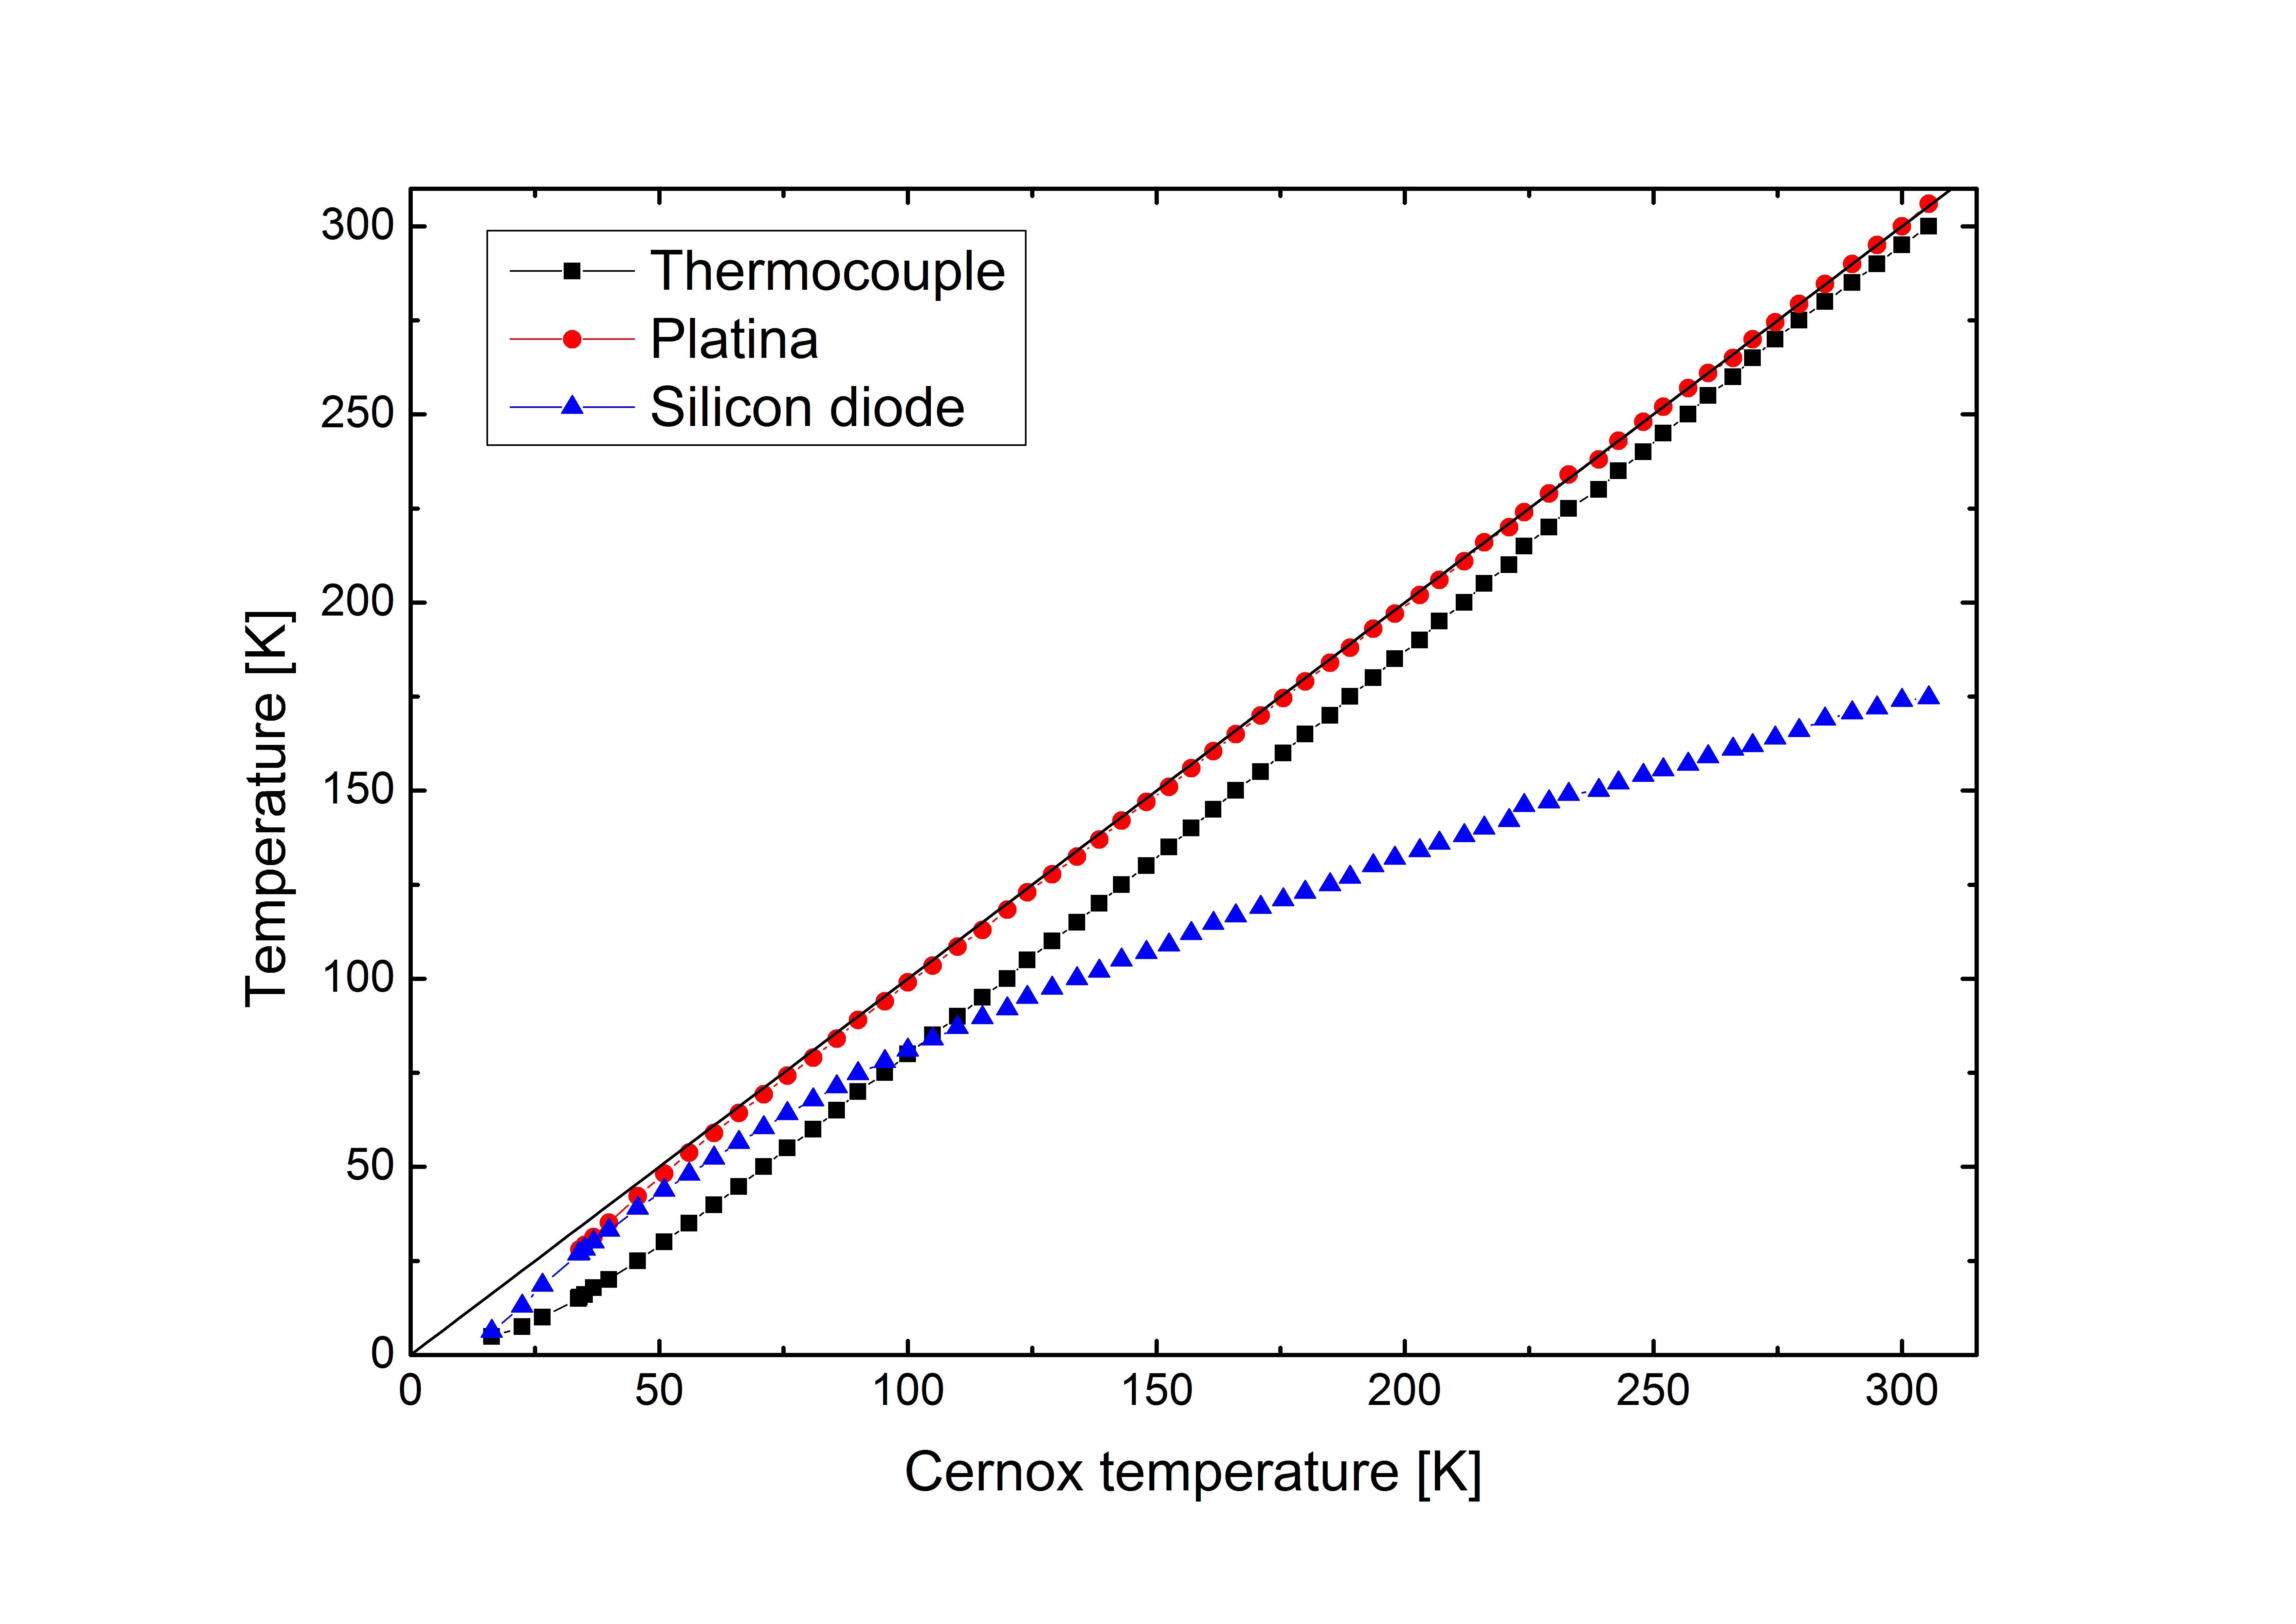
\includegraphics[width=0.8\textwidth]{./png/sensorcalibration}
	\caption{Kalibrace teplotních čidel. Na horizontální ose je skutečná teplota (měřená teplotním čidlem Cernox).}\label{sensor}
\end{figure}


Chladící výkon je vždy stejný a teplota se reguluje pouze topením. Při vypnutém topení dosáhne kryostat nejnižší možné teploty, kterou odhadujeme shora $T<\SI{15}{\kelvin}$. V grafech tato měření označujeme jako $T=\SI{12(3)}{\kelvin}$. Přestože procedura chlazení je vždy stejná, skutečná teplota se může při dvou zchlazeních lišit. Měření, u kterých uvádíme $T<\SI{15}{\kelvin}$, tedy neproběhla nutně při stejné teplotě. Každý typ měření (rozdělení do podkapitol) však proběhl ve stejný den při stejném zchlazení vzorku (bez změny nastavení termostatu).

Kryostat byl napojený na rotační a turbomolekulární vývěvu kvůli dosažení dostatečně nízkého tlaku (před zapnutím chlazení byl tlak \SI{2,5e-6}{\hecto\pascal}).
\chapter{Měření hysterezních smyček}
V této kapitole se věnujeme studiu hysterezních smyček. 
Studujeme pouze tzv. majoritní hysterezní smyčky, které začínají a končí v dostatečně vysokých polích (na koncích smyčky je magnetizace ve směru vnějšího pole).
V majoritních hysterezních smyčkách typicky dochází ke dvěma přeskokům magnetizace, při koercitivních polích $\hcj$ a $\hcd$ \cite{Reichlova}.

Měřením Voigtova jevu a MLD u hysterezních smyček určujeme koercitivní pole $\hcj$ a $\hcd$ a amplitudy přeskoku $A$ a $\Delta B$, ze kterých lze případně určit $\pmld$, součin $\pmld \sin(\xi)$ a směry snadných os.


Měření v nekolineární geometrii na stejném vzorku proběhlo už v práci \cite{Reichlova}, a proto stejný experiment použijeme jako první magnetooptické měření s dvoudimenzionálním elektromagnetem k ověření jeho funkčnosti a použitelnosti.

\section{Metoda měření a zpracování dat} \label{zpracovani_smycek}
Hysterezní smyčky měříme vždy při fixované rovině polarizace $\beta$ a směru vnějšího pole $\phH$.
Znaménko $\hext$ volíme tak, aby kladné hodnoty byly ve směru, který uvádíme. První část smyčky (ze záporných $\hext$ do kladných) označujeme jako \emph{up} a druhou část (z kladných do záporných) \emph{down}.
Up a down zpracováváme zcela odděleně a díky symetrii očekáváme stejné výsledky.

Nejprve vyvážíme můstek na jednom okraji hysterezní smyčky a poté při postupné změně $\hext$ měříme rozdílový a součtový signál, ze kterého vypočítáme $\Delta\beta$ podle \eqref{e:mustek}.


Signál $B$ vypočítáme tak, že součtový signál dělíme jeho střední hodnotou během příslušné části hysterezní smyčky a poté odečteme 1 jako v definici \eqref{e:Bdef}.

Způsob, jakým odečítáme hodnoty $A$, $\Delta B$, $\hcj$ a $\hcd$ je znázorněn na obr. \ref{zpracovani}. Význam veličiny $A_r$ je vysvětlen na str. \pageref{e:Ar}.


V textu dále uváděná chyba veličin $A$, $\Delta B$, $\hcj$ a $\hcd$ je odhadnutá maximální chyba, tj. hranice, za kterou už hodnota na první pohled neodpovídá naměřeným datům.

Průběhy veličin $\Delta \beta$ a $B$ v hysterezních smyčkách, které vykreslujeme, jsme pro lepší přehlednost v některých případech posunuli po vertikální ose do jiných hodnot.

\begin{figure}[htbp]\centering
\qq{	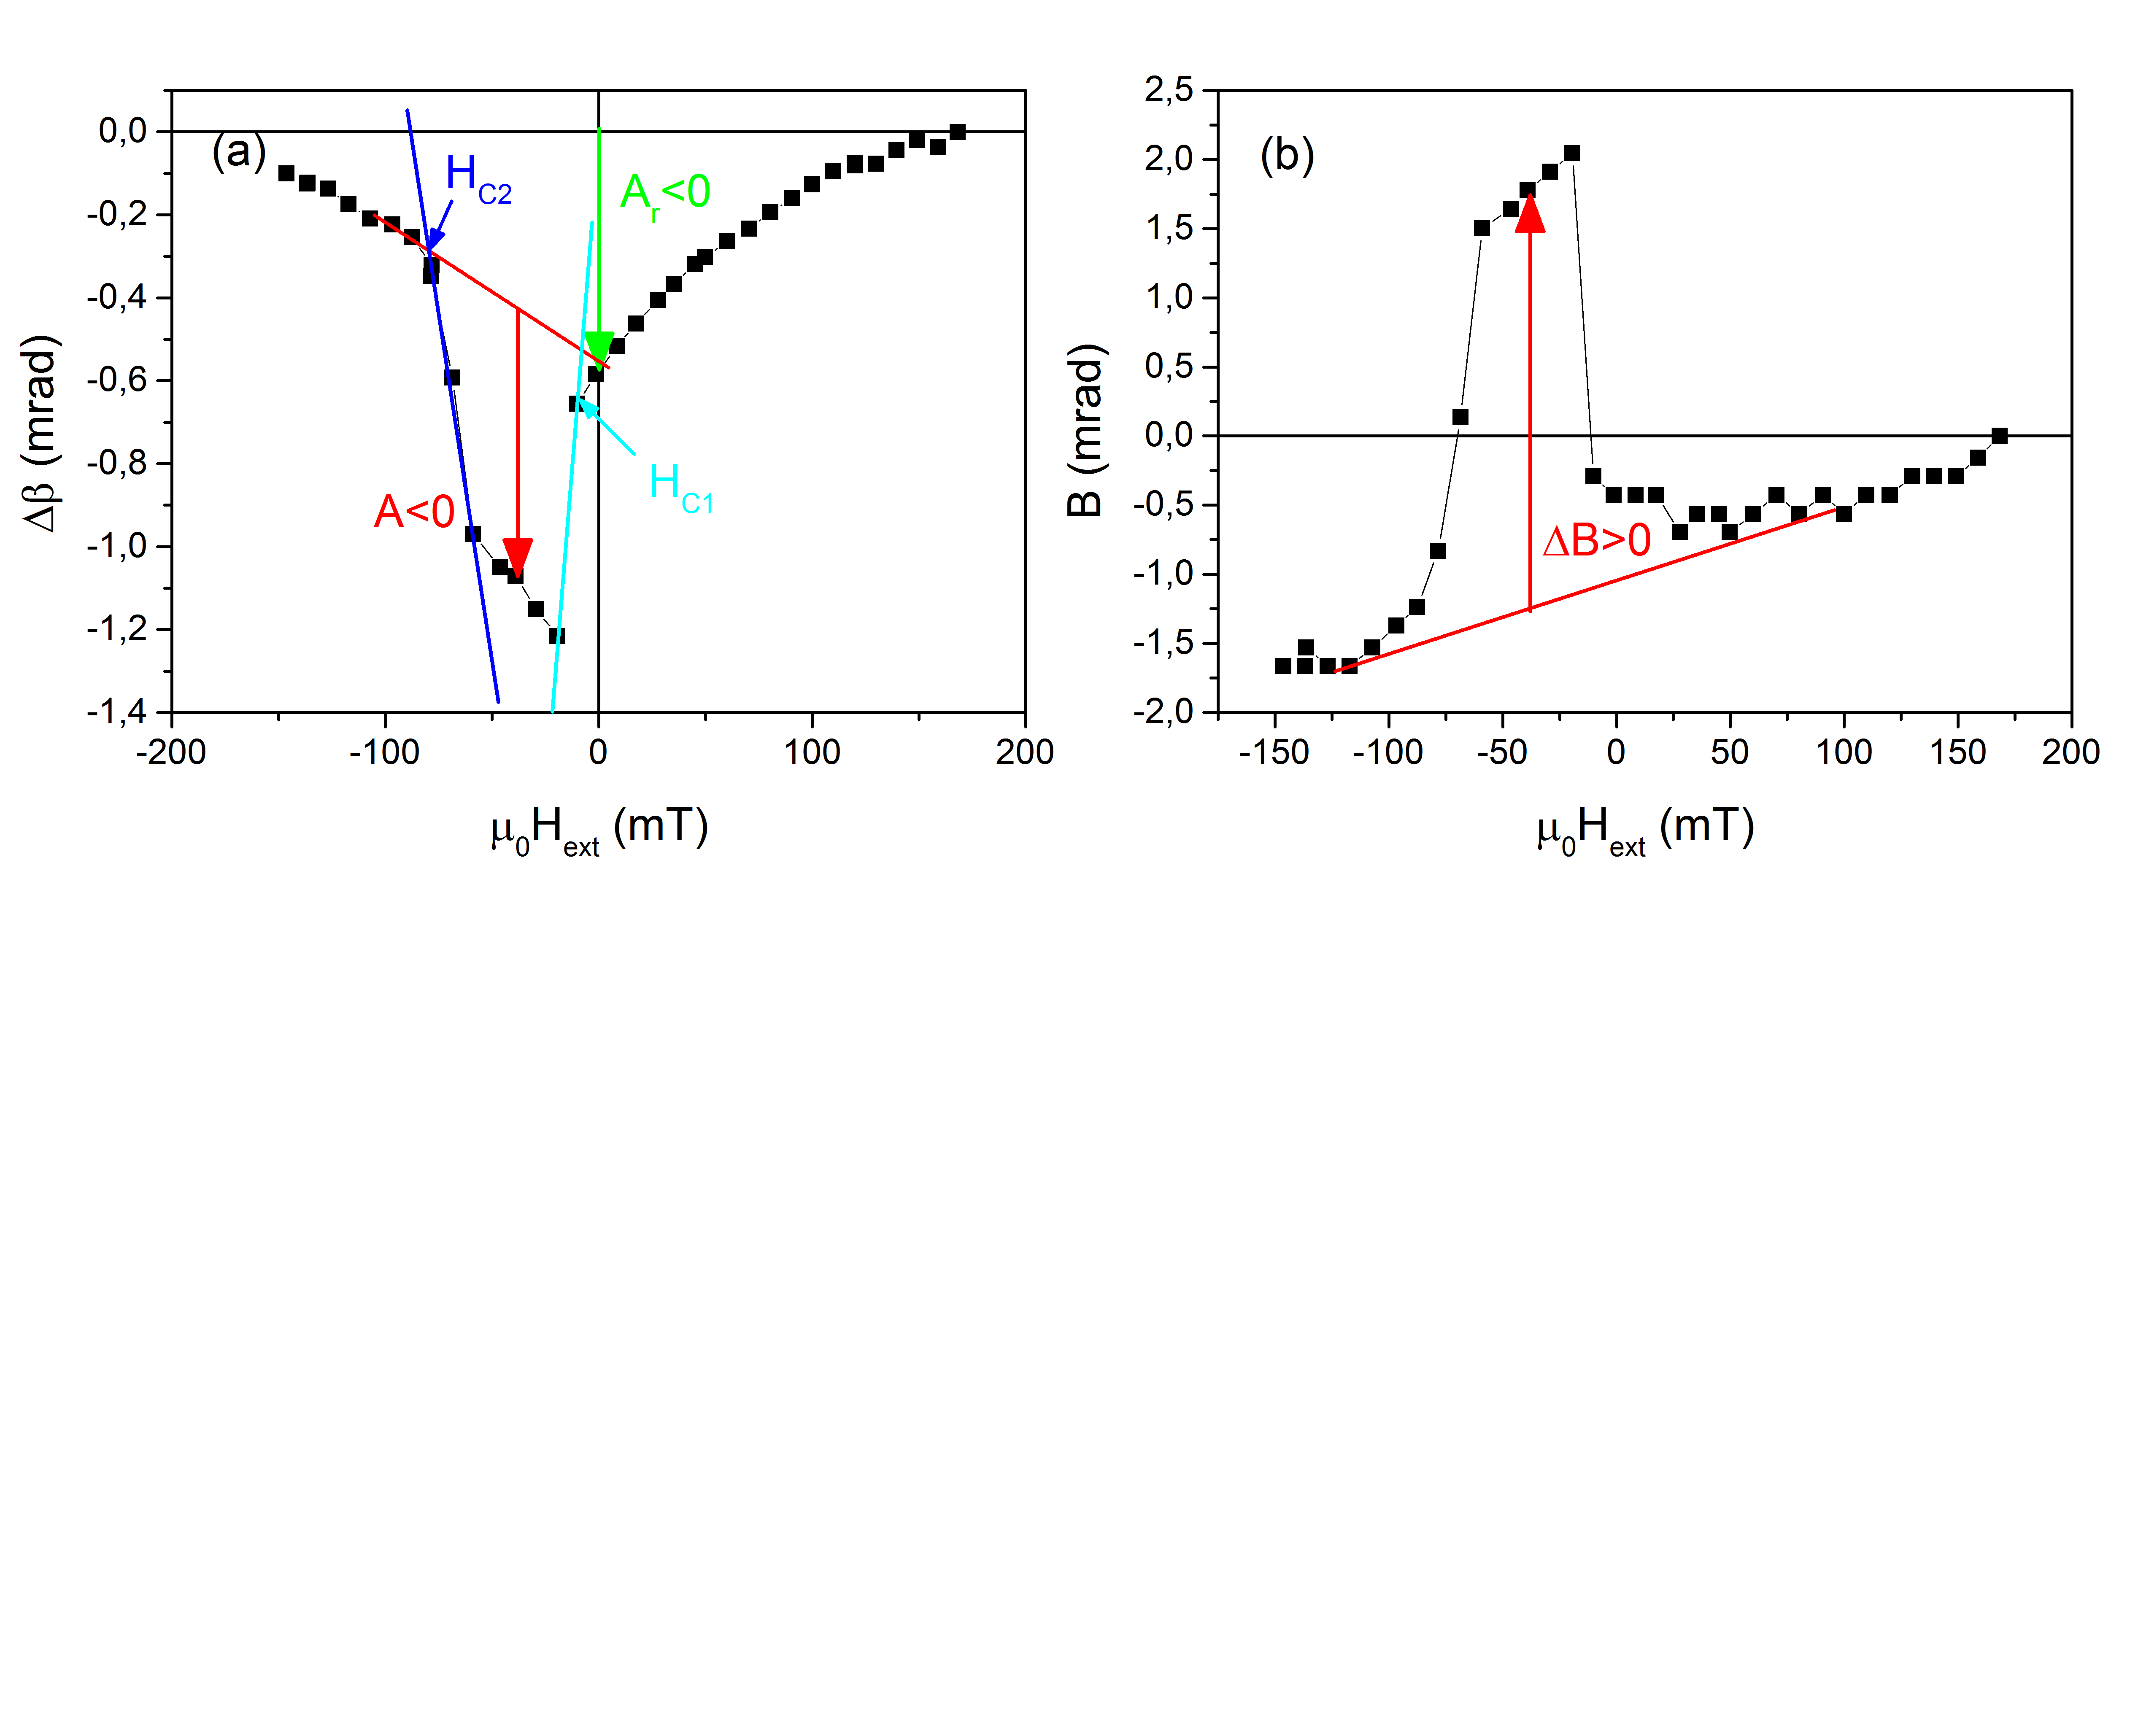
\includegraphics[trim={0 3.43in 0 0}, clip, width=\textwidth]{./png/hyst_zpracovani}}
	\caption{Ilustrace metody určování veličin $A$, $A_r$, $\Delta B$, $\hcj$ a $\hcd$ u hysterezních smyček. Nekolineární geometrie, $\phH=\ang{0}$ pro polarizaci $\beta=\ang{60}$ (a) a $\beta=\ang{30}$ (b).}\label{zpracovani}
\end{figure}

\FloatBarrier


\section{Nekolineární geometrie}
Měřili jsme polarizační závislost hysterezních smyček pro dva směry vnějšího pole $\phH=\ang{0}$ a $\phH=\ang{135}$ při teplotě $T<\SI{15}{\kelvin}$. Intenzita laseru dopadající na vzorek byla \SI{1}{\milli\watt}.

\subsection*{Vnější pole ve směru \ang{135}}
Na obr. \ref{nekol_vysledky_voigt} je typický průběh rozdílového signálu vlivem Voigtova jevu. Polarizační závislost je na obr. \ref{nekol_vysledky_voigt} (b), (c)).


\begin{figure}[htbp]\centering
\qq{	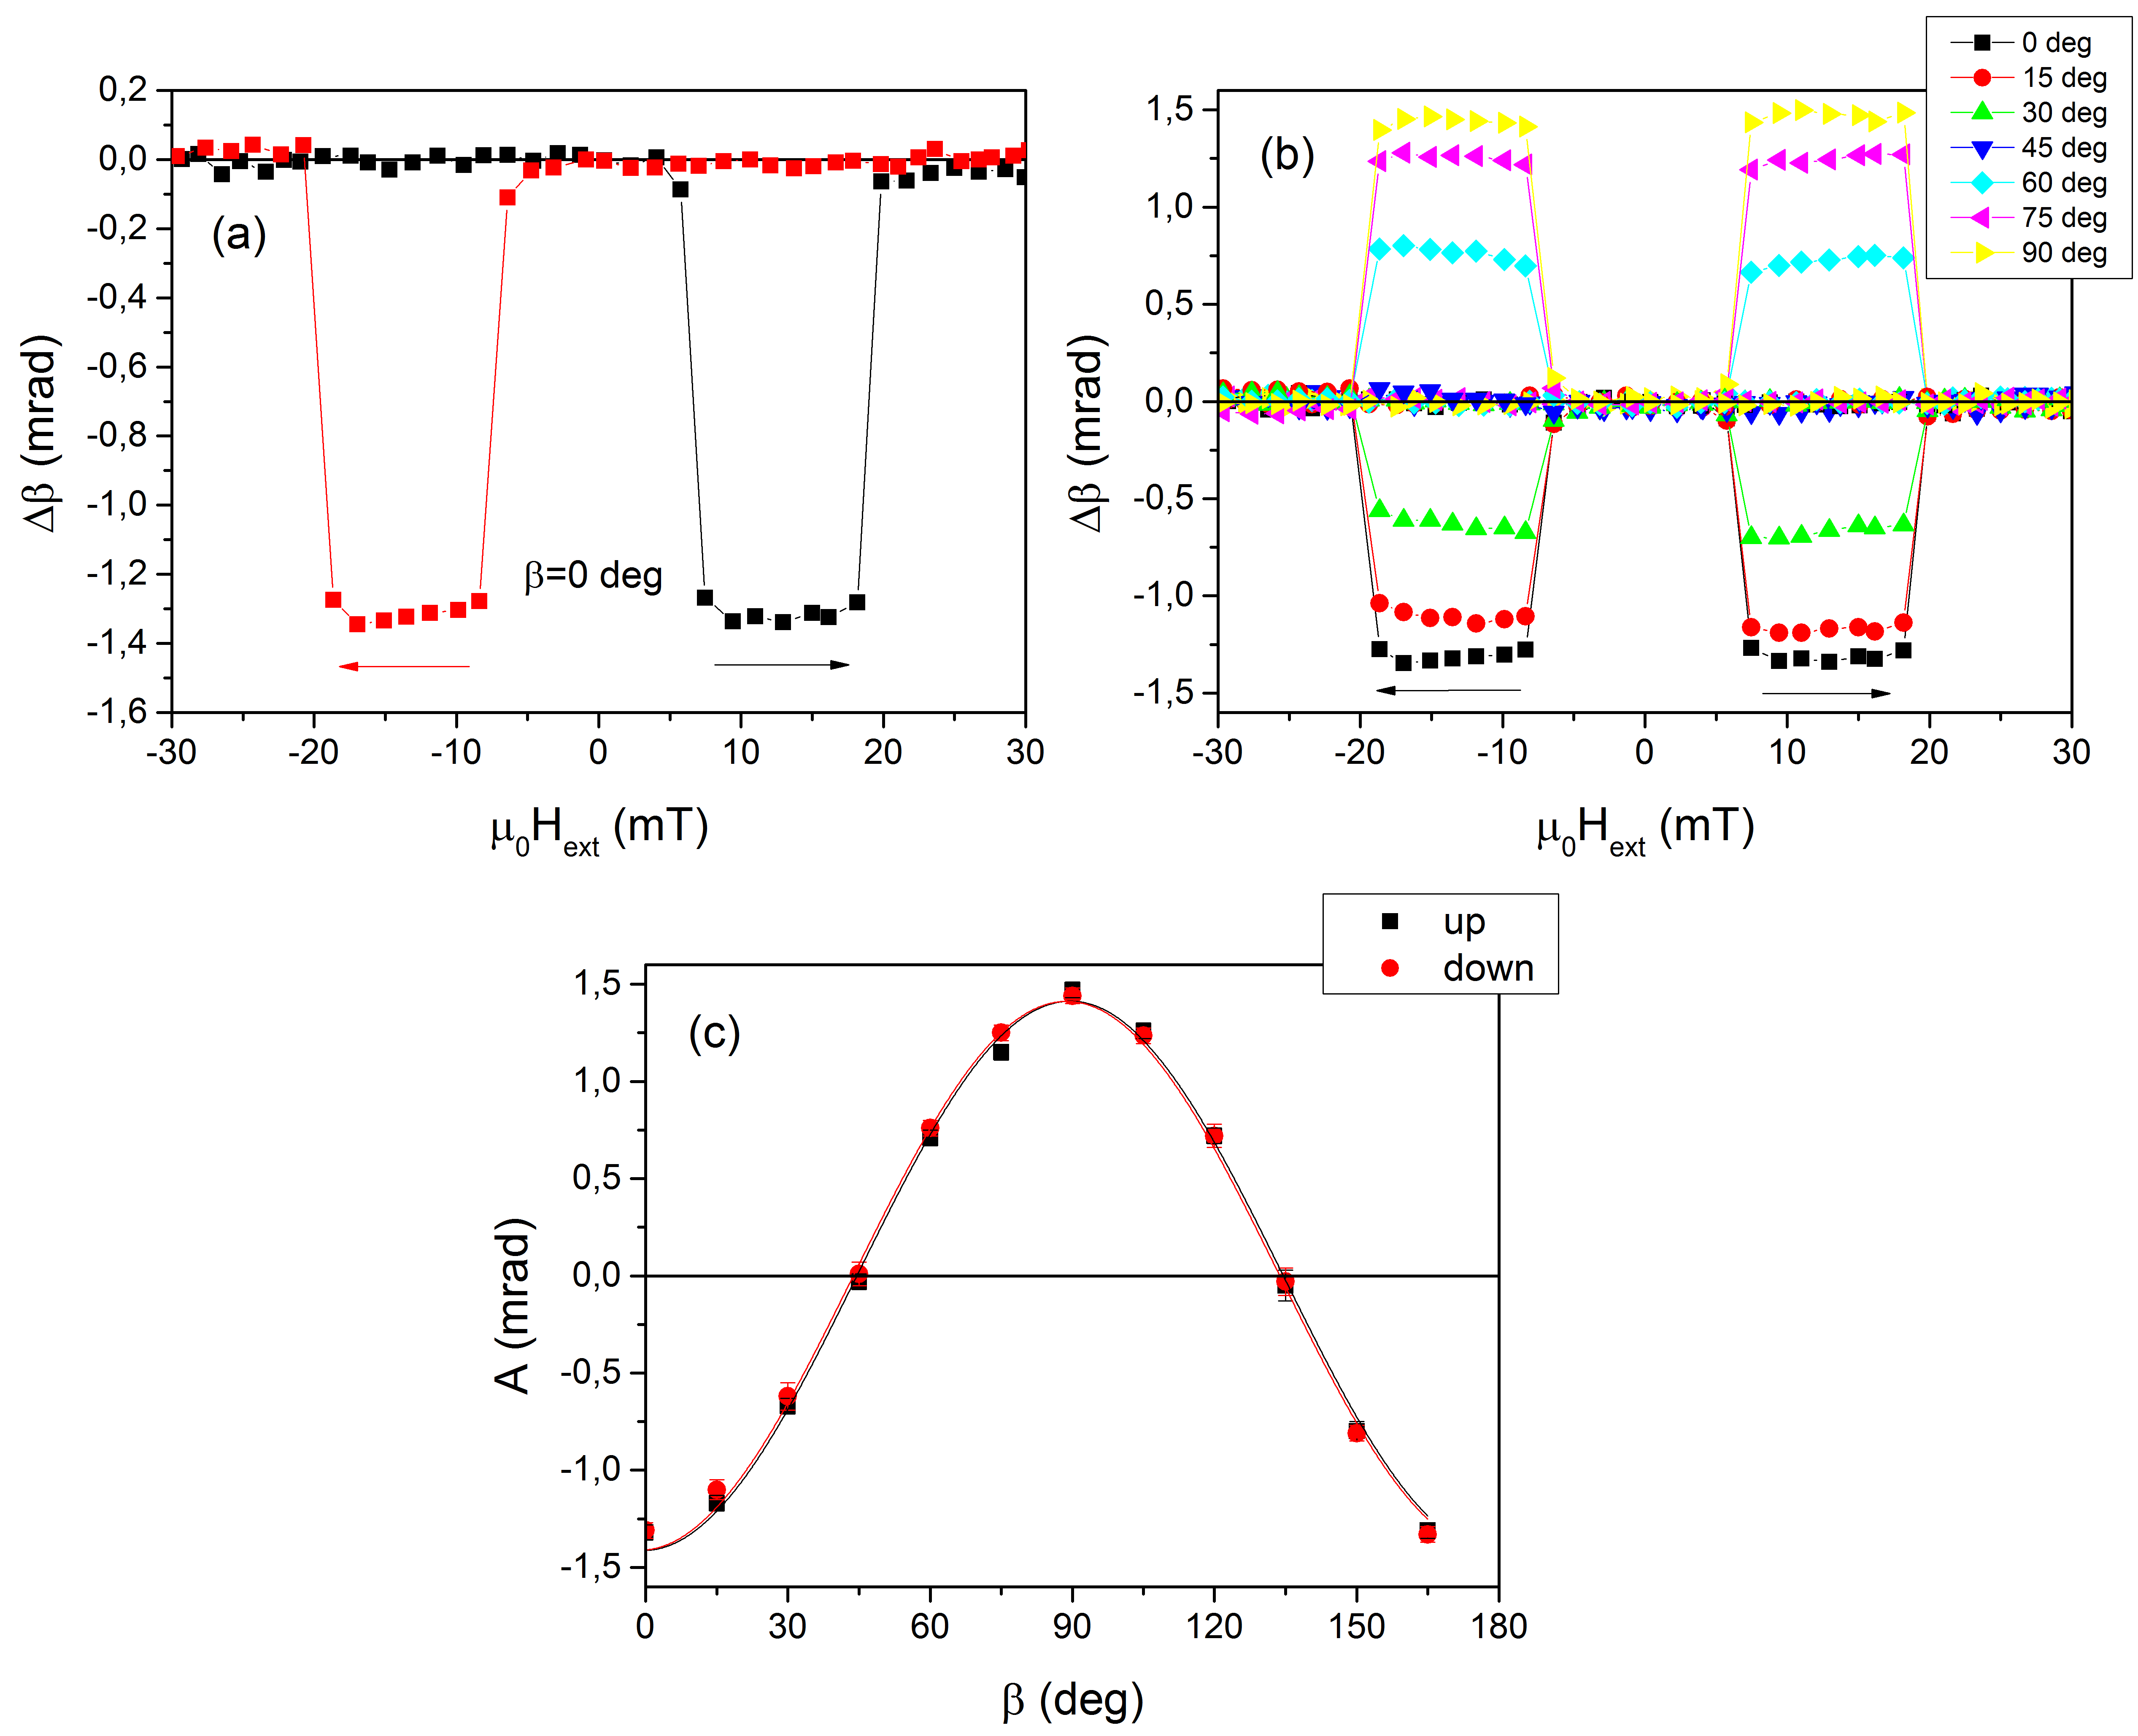
\includegraphics[width=\textwidth]{./png/nekolhyst_135pol_voigt}}
	\caption{Měření Voigtova jevu v hysterezních smyčkách pro $\phH=\ang{135}$ v~nekolineární geometrii. (a) Typická hysterezní smyčka ($\beta=\ang{0}$). (b) Polarizační závislost hysterezních smyček. (c) Polarizační závislost amplitudy $A$ (body), nafitovaná závislost vztahem \eqref{e:amplVoigt} (čára).}\label{nekol_vysledky_voigt}
\end{figure}

V součtovém napětí jsme také pozorovali obdobný signál. Měření probíhalo přibližně hodinu a během ní poměrně rovnoměrně a konzistentně klesala intenzita laseru. Nejdříve byla změřena polarizace $\beta=\ang{0}$ a poté jsme ji po \ang{15} zvyšovali až do $\beta=\ang{165}$. Na obr. \ref{nekol_vysledky_mld} (a) je graf, jak v průběhu měření klesala intenzita. To se projevilo i v samotných hysterezních smyčkách, viz obr. \ref{nekol_vysledky_mld} (b). Intenzita klesá s~časem, který má v up a down měřeních opačný směr.

Intenzita si během celého měření držela stejný trend poklesu, což nám umožnilo jednoduše porovnat hysterezní smyčky pro různé polarizace, viz obr. \ref{nekol_vysledky_mld} (c). Naměřené smyčky jsou vždy vydělené počáteční hodnotou a je odečtena 1 (takže při vyváženém můstku je $B=0$). Odečetli jsme amplitudy přeskoků $\Delta B$, její polarizační závislost je na obr. \ref{nekol_vysledky_mld} (d).

\begin{figure}[htbp]\centering
\qq{	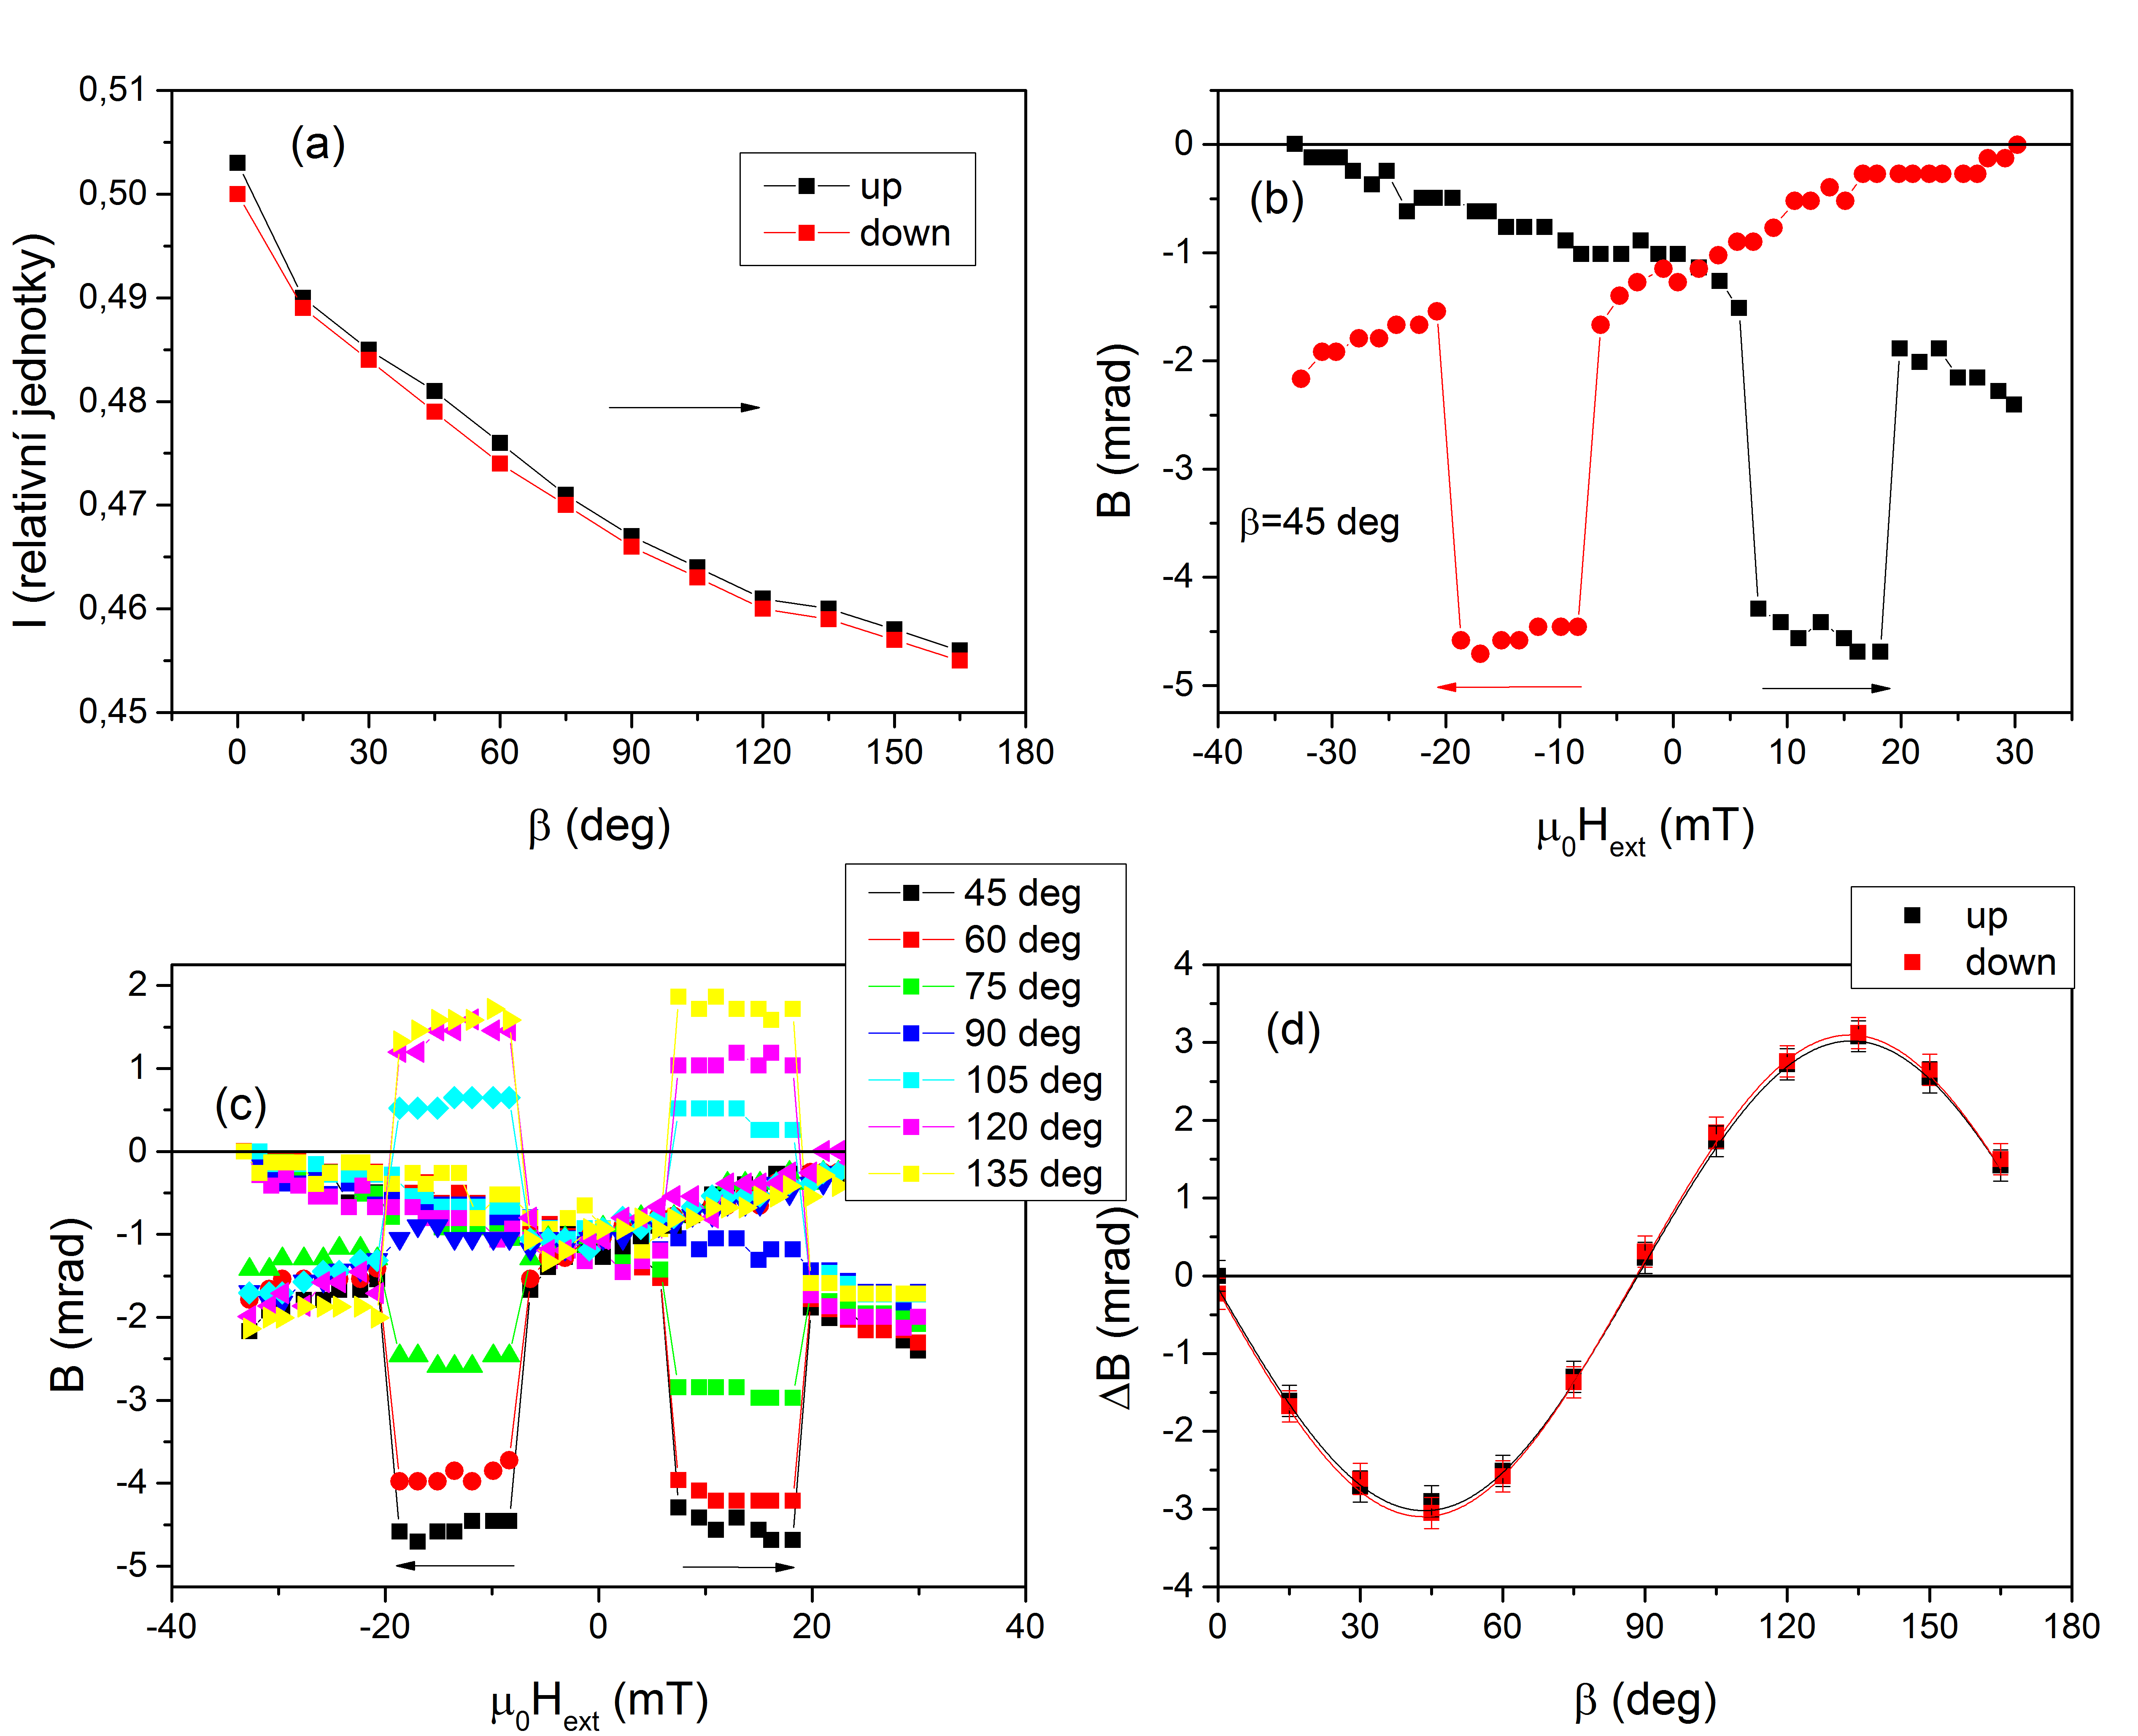
\includegraphics[width=\textwidth]{./png/nekolhyst_135pol_mld}}
	\caption{Měření MLD v hysterezních smyčkách pro $\phH=\ang{135}$ v nekolineární geometrii. (a) Průměrná intenzita laseru při měření jednotlivých polarizací. (b) Typická hysterezní smyčka ($\beta=\ang{45}$). (c) Polarizační závislost hysterezních smyček. (d) Polarizační závislost amplitudy $\Delta B$ (body), nafitovaná závislost vztahem \eqref{e:amplMLD} (čára).}\label{nekol_vysledky_mld}
\end{figure}


\FloatBarrier

\subsection*{Vnější pole ve směru \ang{0}}

V tomto směru se oproti $\phH=\ang{135}$ uplatňuje nový jev. Z obr. \ref{souradna_soustava_vzorek} (b) je vidět, že směr \ang{0} se ani přibližně neshoduje s žádnou snadnou osou magnetizace. Aplikací vnějšího pole $\hext$ dochází k vychýlení preferovaného směru magnetizace ze snadné osy. Vychýlení magnetizace závisí spojitě na intenzitě pole, což má za následek dodatečný magnetooptický signál. Hysterezní smyčku pak pozorujeme na trojúhelníkovém pozadí jako na obr. \ref{nekol_vysledky0_voigt} (a). Tento jev charakterizujeme hodnotou $A_r$, kterou definujeme jako (viz obr. \ref{zpracovani})
\begin{equation} \label{e:Ar}
A_{r}:=\Delta \beta_\text{vyvážený můstek} - \Delta \beta_{\hext=0} \,.
\end{equation}
Polarizační závislost $A_r$ je na obr. \ref{nekol_vysledky0_voigt} (c).
$A_r (\beta)$ jsme také proložili funkcí $a\sin(\beta-b)$ s parametry $a$, $b$.

Amplitudu přeskoku $A$ určíme z grafu vzhledem k interpolovanému pozadí zmiňovaného jevu.


\begin{figure}[htbp]\centering
\qq{	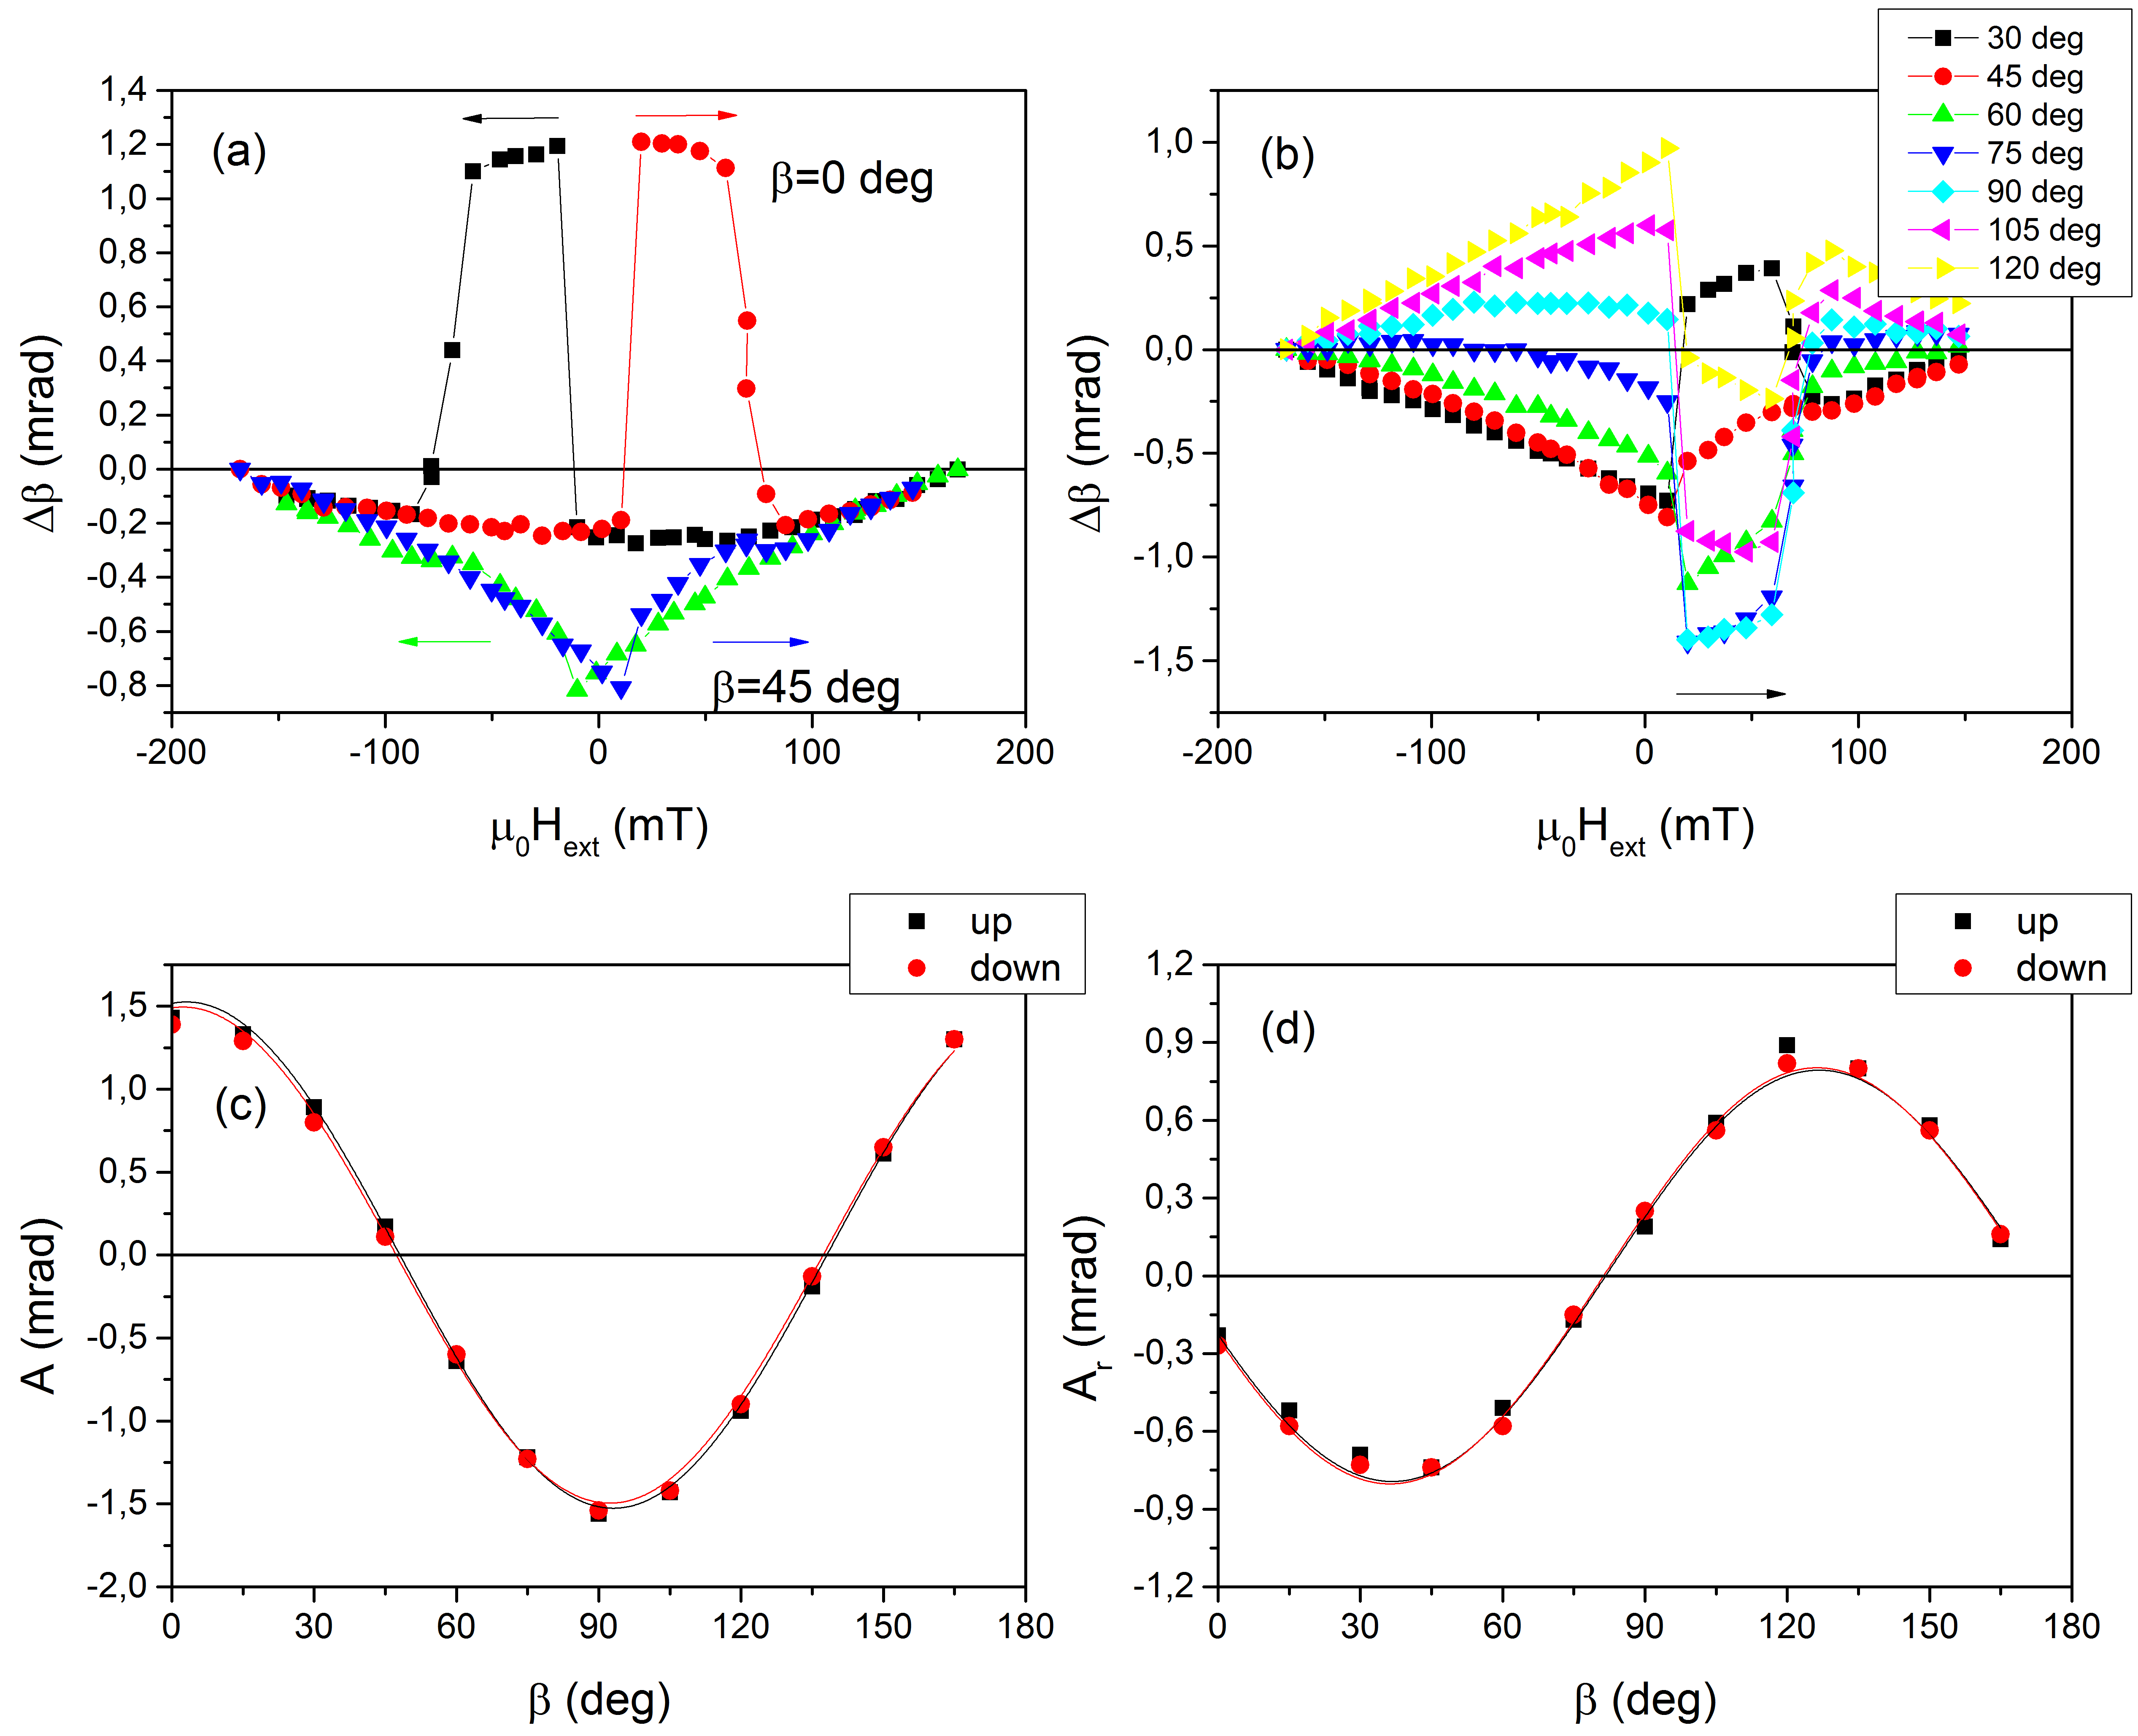
\includegraphics[width=\textwidth]{./png/nekolhyst_0pol_voigt}}
	\caption{Měření Voigtova jevu v hysterezních smyčkách pro $\phH=\ang{0}$ v nekolineární geometrii. (a) Typická hysterezní smyčka ($\beta=\ang{0}$ a \ang{45}). (b) Hysterezní smyčky pro vybrané polarizace. (c) Polarizační závislost amplitudy přeskoku $A$ (body), nafitovaná závislost vztahem \eqref{e:amplVoigt} (čára). (d) Polarizační závislost $A_r$ (body), nafitovaná závislost funkcí $a\sin(\beta-b)$ (čára).}\label{nekol_vysledky0_voigt}
\end{figure}

V součtovém signálu jsou opět zřetelné hysterezní smyčky na pozadí stále klesající intenzity. Data jsme zpracovali stejným způsobem jako pro $\phH=\ang{135}$. Naměřená data jsou na obr. \ref{nekol_vysledky0_mld} (a-d). Jev s trojúhelníkovým profilem je opět přítomný (viz obr. \ref{nekol_vysledky0_mld} (c)), ale na pozadí klesající intenzity je obtížné ho dobře změřit.

Na tomto místě je vhodné poznamenat, že data naměřená pro $\phH=\ang{135}$ a \ang{0} mají stejnou symetrii (tj. polohu extrémů a uzlových bodů), ale liší se jejich znaménko (viz např. obr. \ref{nekol_vysledky_voigt} (c) a \ref{nekol_vysledky0_voigt} (c)).

\begin{figure}[htbp]\centering
\qq{	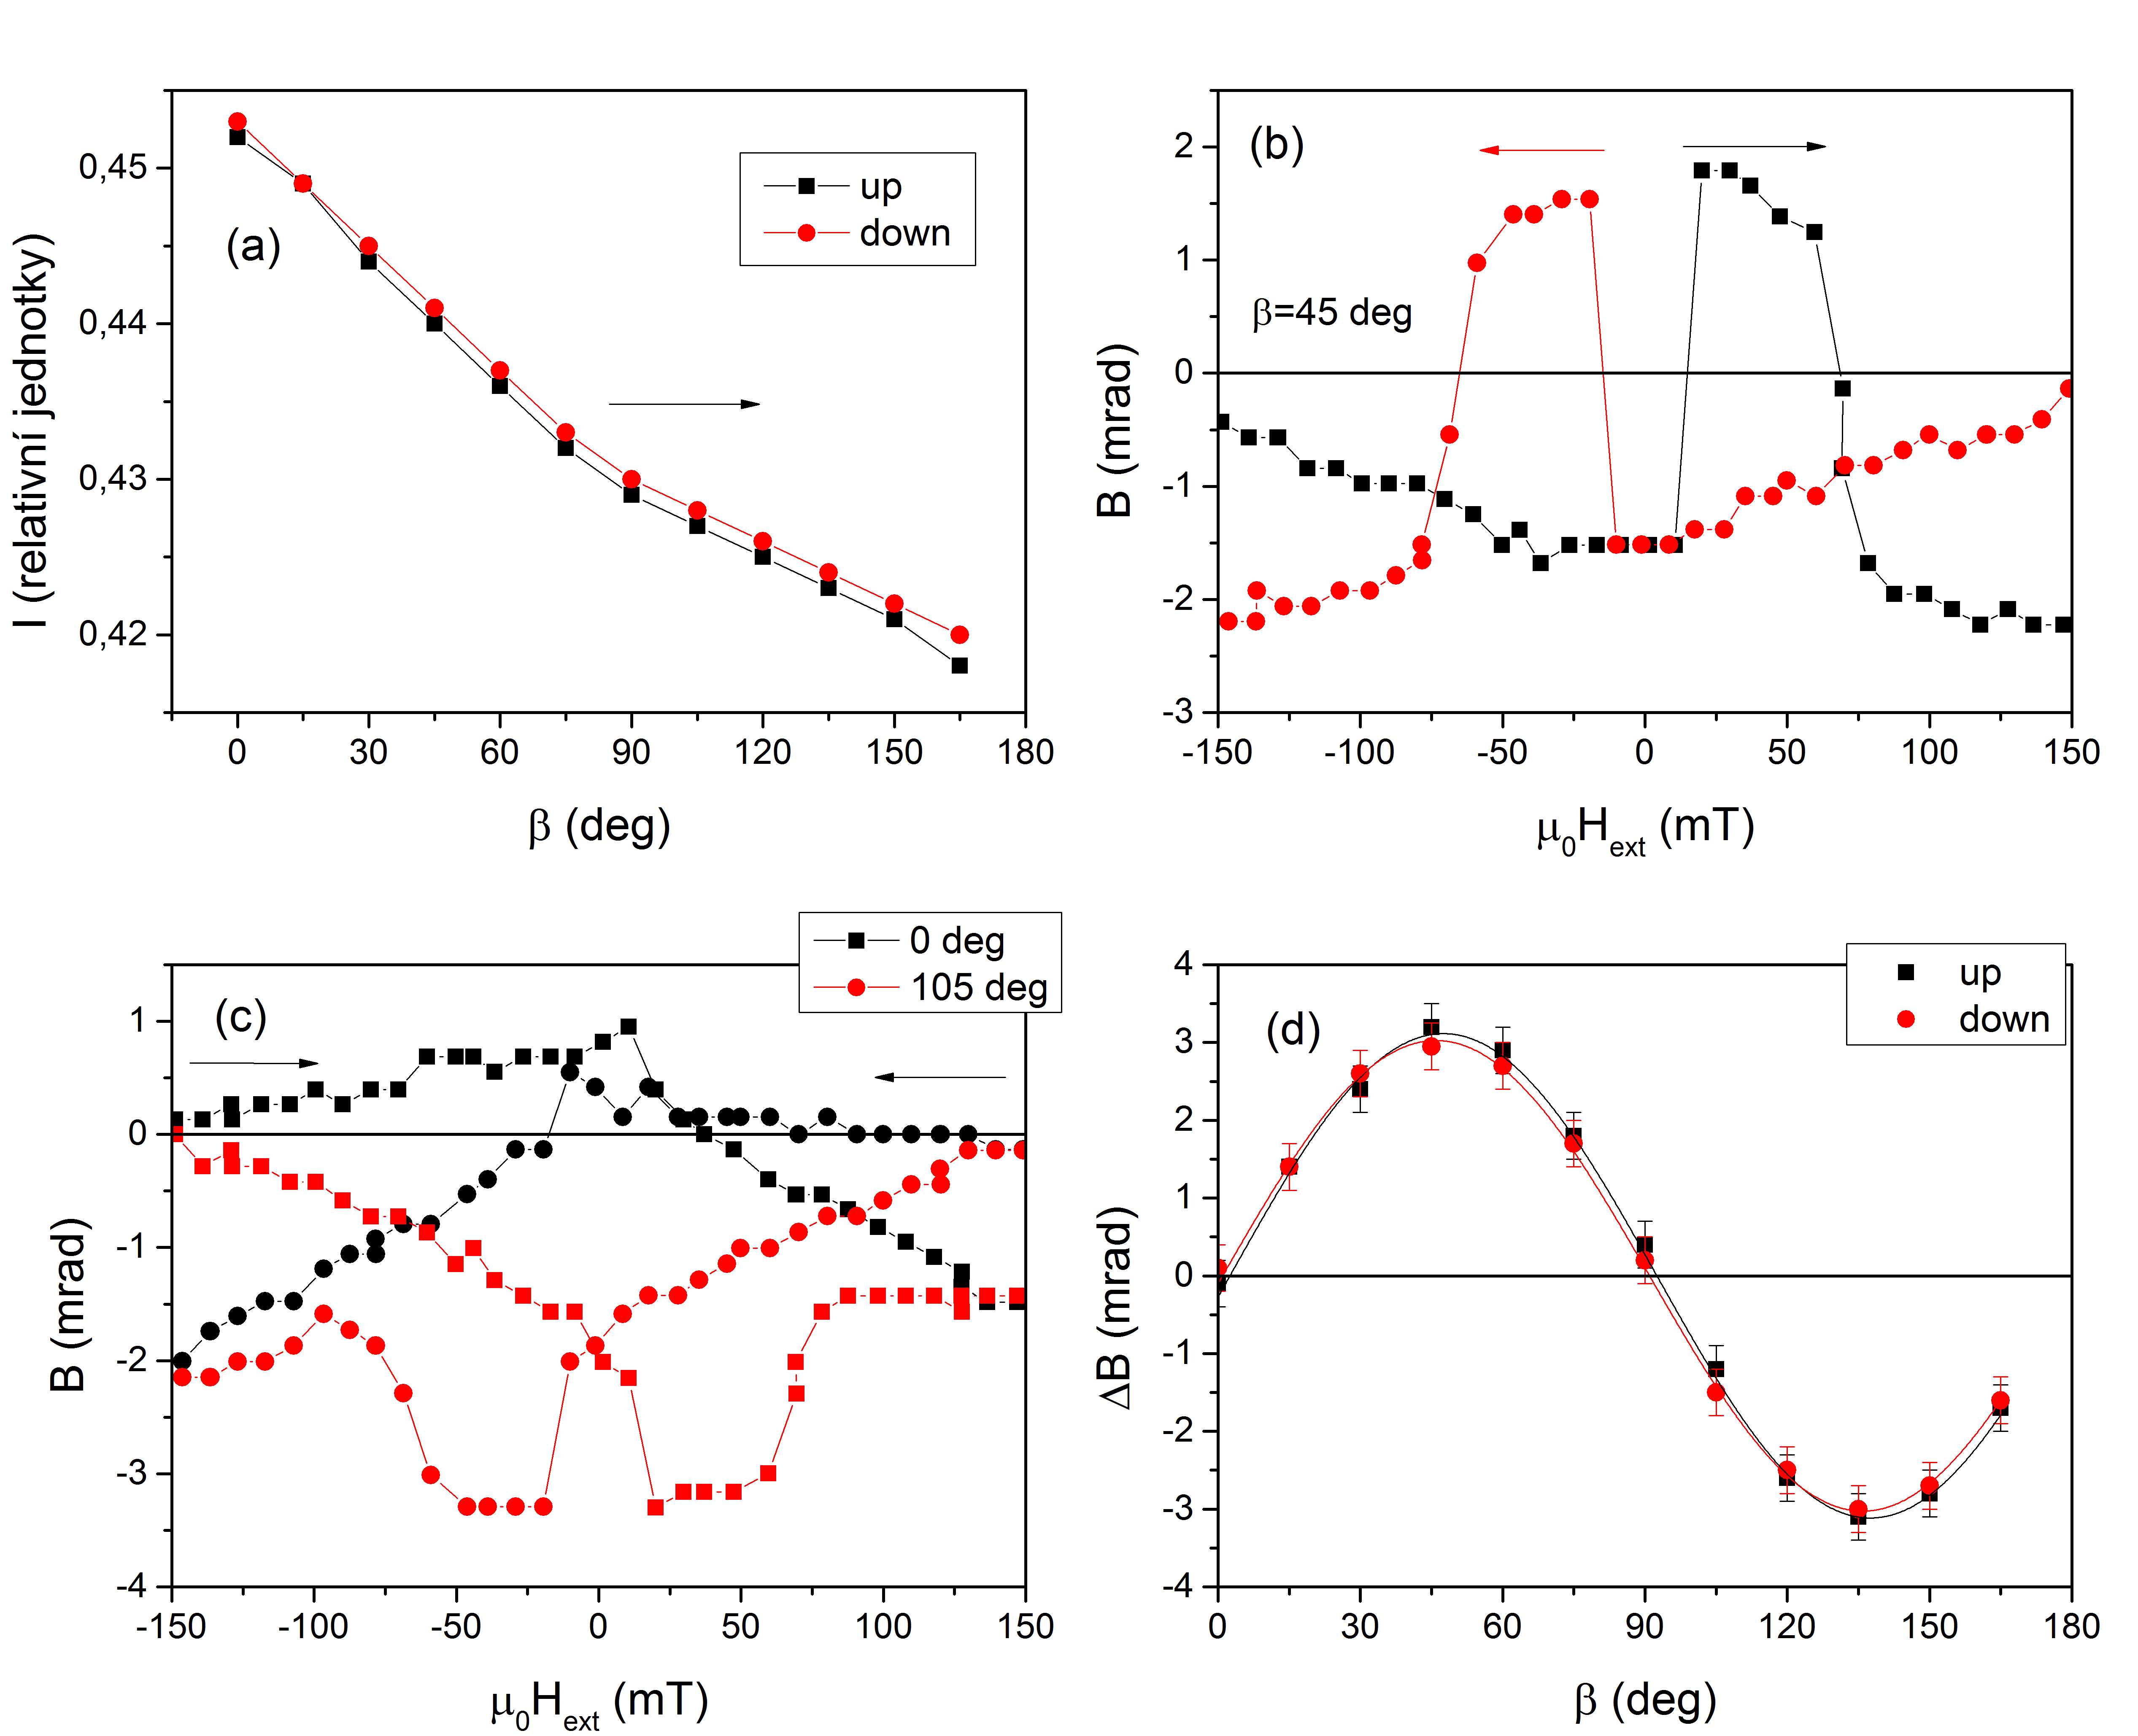
\includegraphics[width=\textwidth]{./png/nekolhyst_0pol_mld}}
	\caption{Měření MLD v hysterezních smyčkách pro $\phH=\ang{0}$ v nekolineární geometrii. (a) Průměrná intenzita laseru při měření jednotlivých polarizací. (b) Typická hysterezní smyčka ($\beta=\ang{0}$). (c) Vybrané hysterezní smyčky $\beta=\ang{0}$, \ang{105}. (d) Polarizační závislost amplitudy $\Delta B$ (body), nafitovaná závislost vztahem \eqref{e:amplMLD} (čára).}\label{nekol_vysledky0_mld}
\end{figure}

V tabulce \ref{tab_nekol_hyst} uvádíme souhrn fitováním určených hodnot jednotlivých parametrů ve vztazích \eqref{e:amplVoigt} a \eqref{e:amplMLD}.


\begin{table}[htbp]	
	\centering	
	\begin{tabular}{c||cc|cc|cc}
		& & & \multicolumn{2}{c|}{fit Voigtův jev} & \multicolumn{2}{c}{fit MLD} \\
		$\phH$ & $\mu_0\hcj$ & $\mu_0\hcd$ & $\pmld \sin\xi$ & $\gamma$ & $\pmld \sin\xi$ & $\gamma$ \\
		(deg) & (mT) & (mT) & (\si{\milli\radian}) & (deg) & (\si{\milli\radian}) & (deg) \\ \hline
		135 up & \num{5,5(4)} & \num{19,0(5)} & \num{-0,70(5)} & \num{89.5(10)} & \num{-0,75(4)} & \num{88,5(10)} \\
		135 down & \num{5,8(4)} & \num{19,8(8)} & \num{-0,70(5)} & \num{88,8(15)} & \num{-0,77(4)} & \num{88,2(10)} \\ \hline
		0 up & \num{15,0(40)} & \num{83(4)} & \num{-0,76(4)} & \num{93,1(10)}& \num{-0,78(5)} & \num{92,5(15)} \\
		0 down & \num{14,5(40)} & \num{81(3)} & \num{-0,75(5)} & \num{92,3(15)} & \num{-0,76(4)}& \num{90,9(10)} \\
	\end{tabular}
	\caption{Měření hysterezních smyček v nekolineární geometrii. U $\phH=\ang{135}$ jsme změnili znaménko $\pmld \sin\xi$, protože dochází k přeskoku v opačném směru než předpokládají vztahy \eqref{e:amplVoigt} a \eqref{e:amplMLD}. V tomto případě platí stejný vztah s~opačným znaménkem.}
	\label{tab_nekol_hyst}
\end{table}

Z této tabulky je patrné, že veškeré získané hodnoty jsou v rámci chyby stejné. Dále je z tohoto měření možné určit, s jakou přesností byl vzorek skutečně nalepen v požadované orientaci --- situaci znázorněné na obr. \ref{souradna_soustava_vzorek} totiž odpovídá $\gamma=\ang{90}$ a průměrná experimentálně určená hodnota $\gamma=\num{90,5(17)}^\circ$.


\FloatBarrier
\section{Kolineární geometrie} \label{kap_kolinearni}
V kolineární geometrii jsme provedli tři druhy měření hysterezních smyček. 
\begin{itemize}
\item Polarizační závislost pro $\phH=\ang{135}$ a $T<\SI{15}{\kelvin}$ pro ověření funkčnosti a porovnání s nekolineární geometrií.
\item Závislost na směru vnějšího pole $\phH \in (\ang{0},\ang{360})$ při $T<\SI{15}{\kelvin}$ a fixovaném $\gamma-\beta=\ang{90}$ (maximální Voigtův jev a nulové MLD).
\item Teplotní závislost pro $\phH=\ang{135}$ a fixované polarizaci $\beta=\ang{0}$ (maximální Voigtův jev a nulové MLD).
\end{itemize}


\subsection{Polarizační závislost při vnějším poli ve směru \ang{135}}
Měření proběhlo při teplotě $T<\SI{15}{\kelvin}$ a intenzita laseru dopadajícího na vzorek byla \SI{2}{\milli\watt}.

Na obr. \ref{kol_vysledky_voigt} (a) je typický průběh Voigtova jevu. Na obr. \ref{kol_vysledky_voigt} (b) jsou hysterezní smyčky pro několik vybraných polarizací. Polarizační závislost amplitudy přeskoku $A$ je vykreslena na obr. \ref{kol_vysledky_voigt} (c). V tabulce \ref{tab_kol_hyst135} jsou shrnuté získané výsledky.

\begin{figure}[htbp]\centering
\qq{	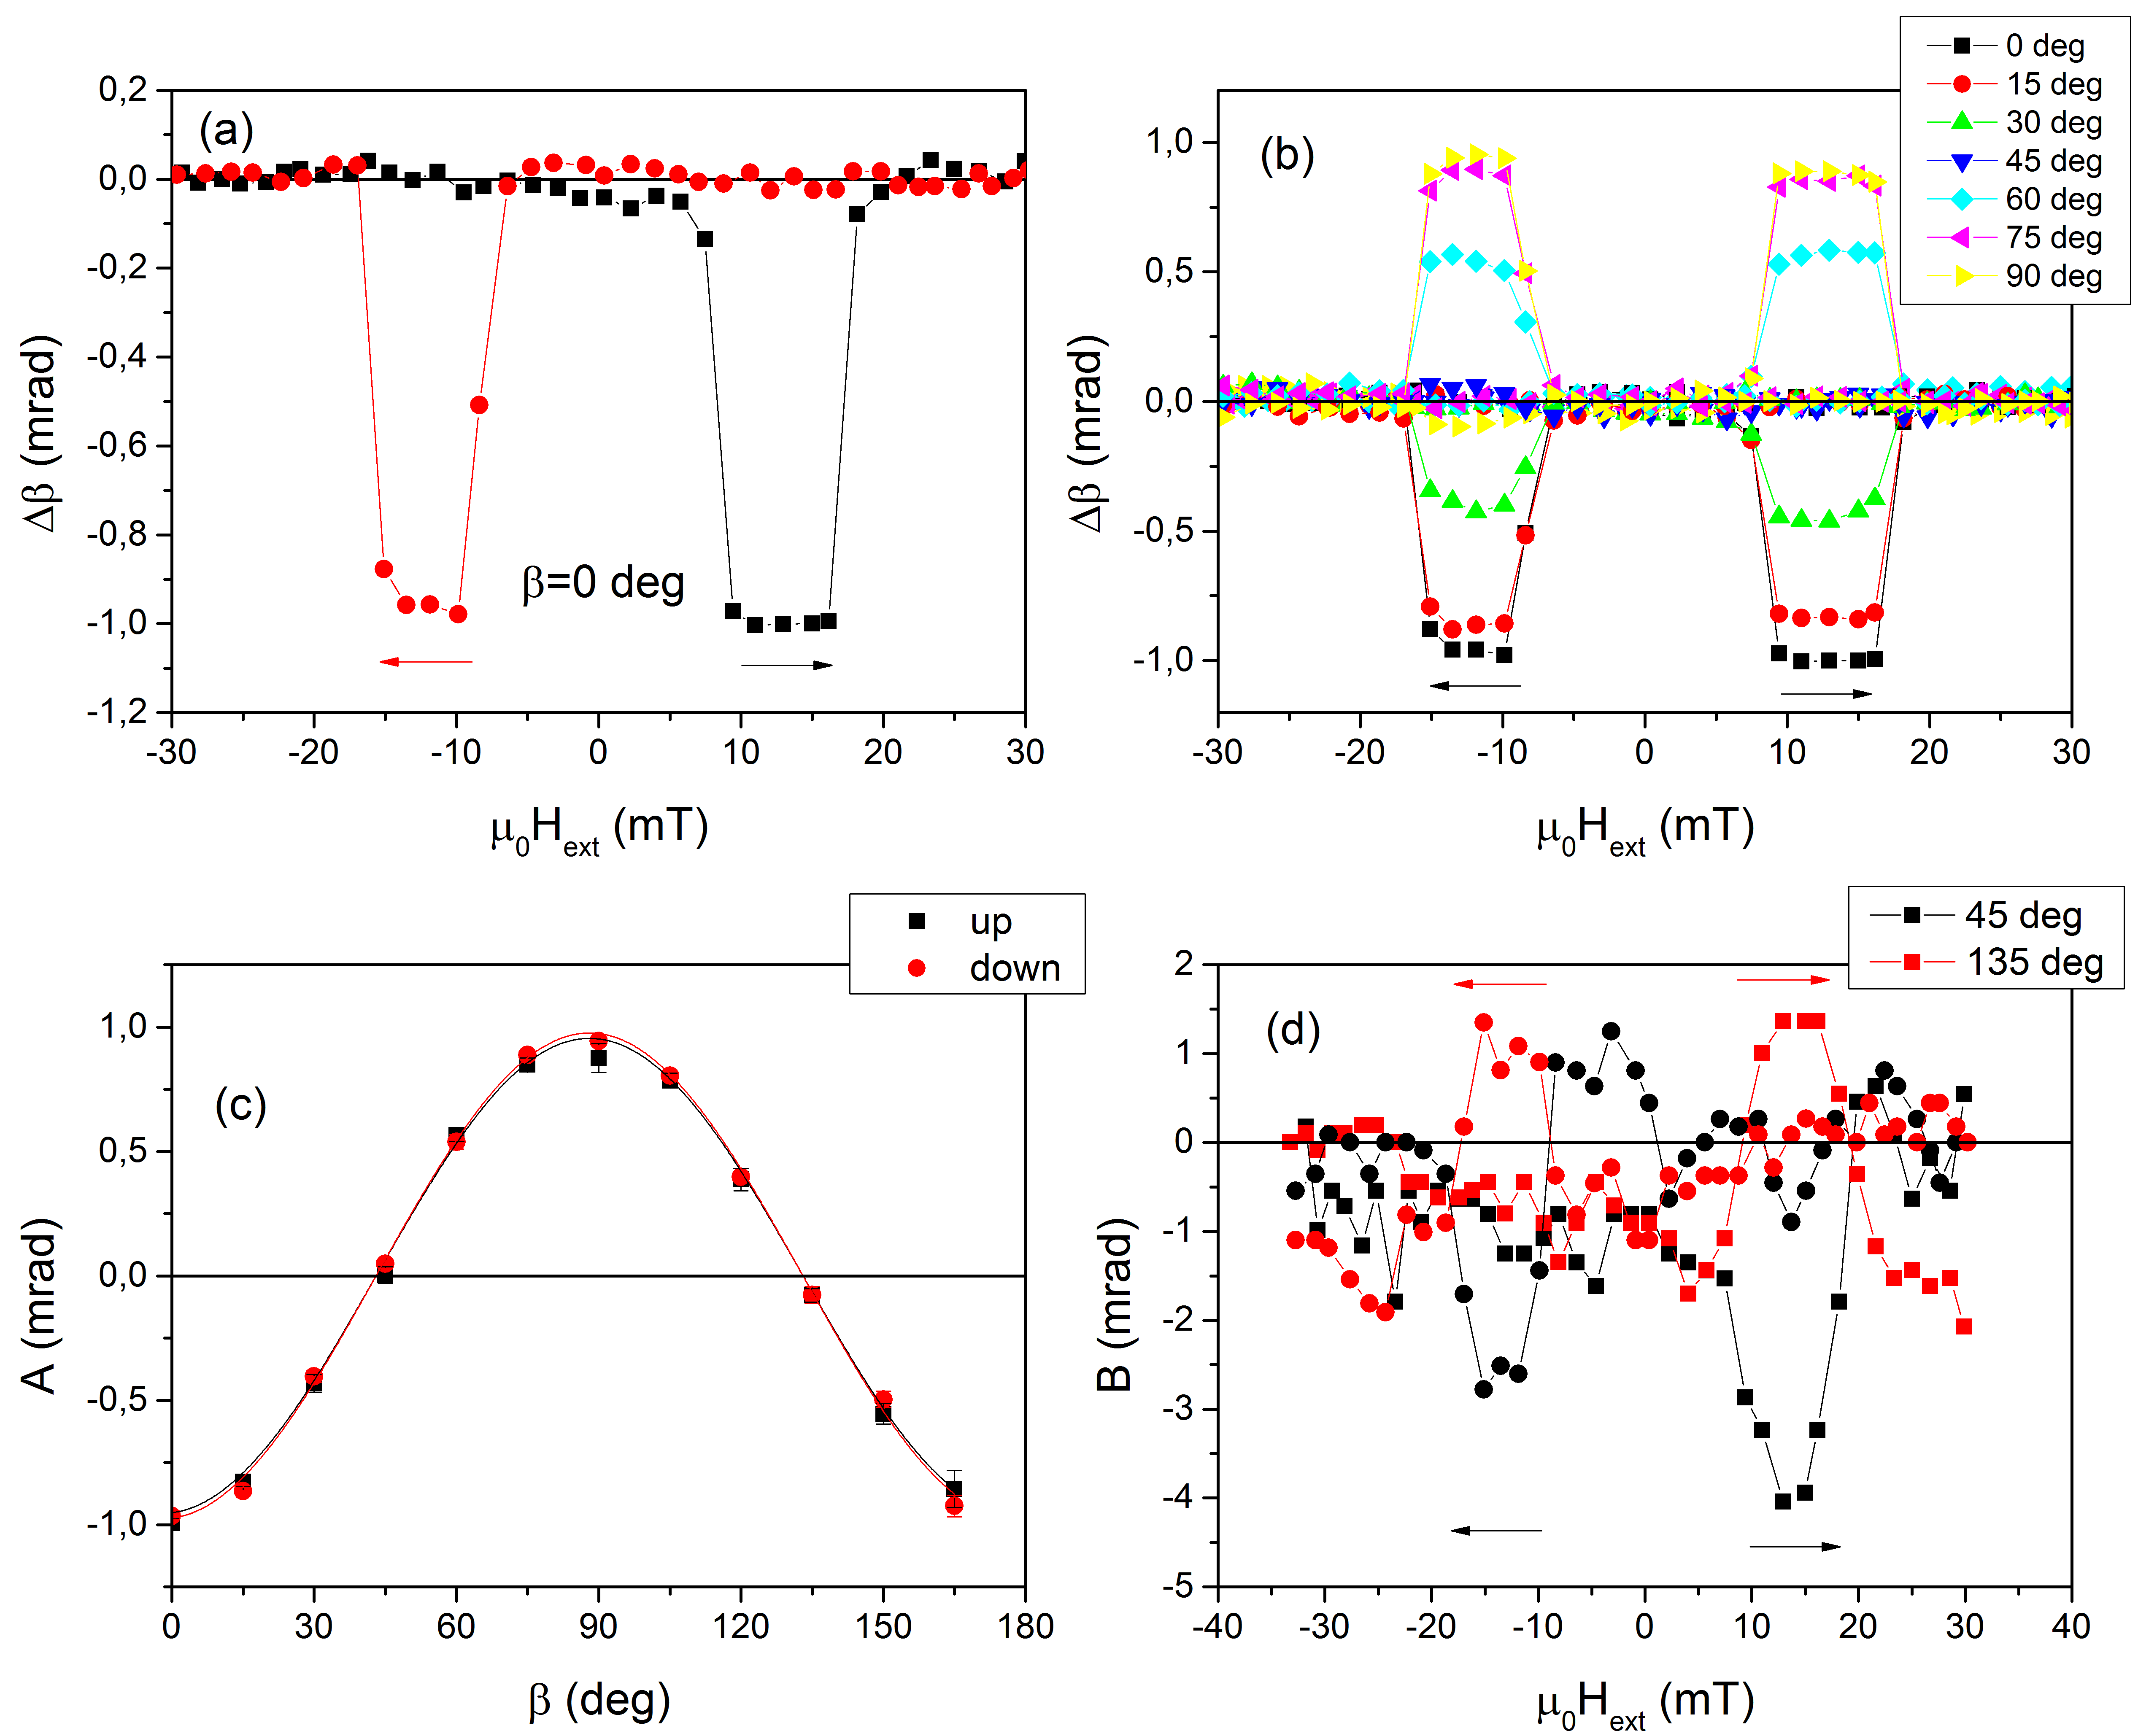
\includegraphics[width=\textwidth]{./png/kolhyst_135pol}}
	\caption{Měření Voigtova jevu v hysterezních smyčkách pro $\phH=\ang{135}$ v~kolineární geometrii. (a) Typická hysterezní smyčka ($\beta=\ang{0}$). (b) Polarizační závislost hysterezních smyček. (c) Polarizační závislost amplitudy $A$ (body), nafitovaná závislost vztahem \eqref{e:amplVoigt} (čára). (d) Součtový signál pro vybrané polarizace.}\label{kol_vysledky_voigt}
\end{figure}

\begin{table}[htbp]	
	\centering	
	\begin{tabular}{c||cc|cc}
		& & & \multicolumn{2}{c}{fit Voigtův jev} \\
		 & $\mu_0\hcj$ & $\mu_0\hcd$ & $\pmld \sin\xi$ & $\gamma$ \\
		 & (mT) & (mT) & (\si{\milli\radian}) & (deg)  \\ \hline
		up & \num{6,8(4)} & \num{17,6(6)} & \num{-0,48(4)} & \num{88,1(15)} \\
		down & \num{7,1(6)} & \num{16,5(7)} & \num{-0,49(3)} & \num{88,1(10)} \\
	\end{tabular}
	\caption{Měření hysterezních smyček v kolineární geometrii pro $\phH=\ang{135}$. Změnili jsme znaménko $\pmld \sin\xi$, protože dochází k přeskoku v opačném směru než předpokládá vztah \eqref{e:amplVoigt}}
	\label{tab_kol_hyst135}
\end{table}

V součtovém signálu je sice patrný MLD signál, ale je téměř na úrovni šumu a tak ho nezpracováváme, viz obr. \ref{kol_vysledky_voigt} (d). Vybrané polarizace jsou ty, u kterých by MLD mělo být nejsilnější.

Ve srovnání s měřením v nekolineární geometrii (viz obr. \ref{kol_nekol}) je patrné, že toto měření proběhlo při vyšší teplotě (viz níže). Koercitivní pole jsou nižší a $|\pmld|$ také. To mohlo být způsobeno, kromě odlišného zchlazení vzorku kryostatem, také vyšším výkonem použitého laseru.

\begin{figure}[htbp]\centering
\qq{	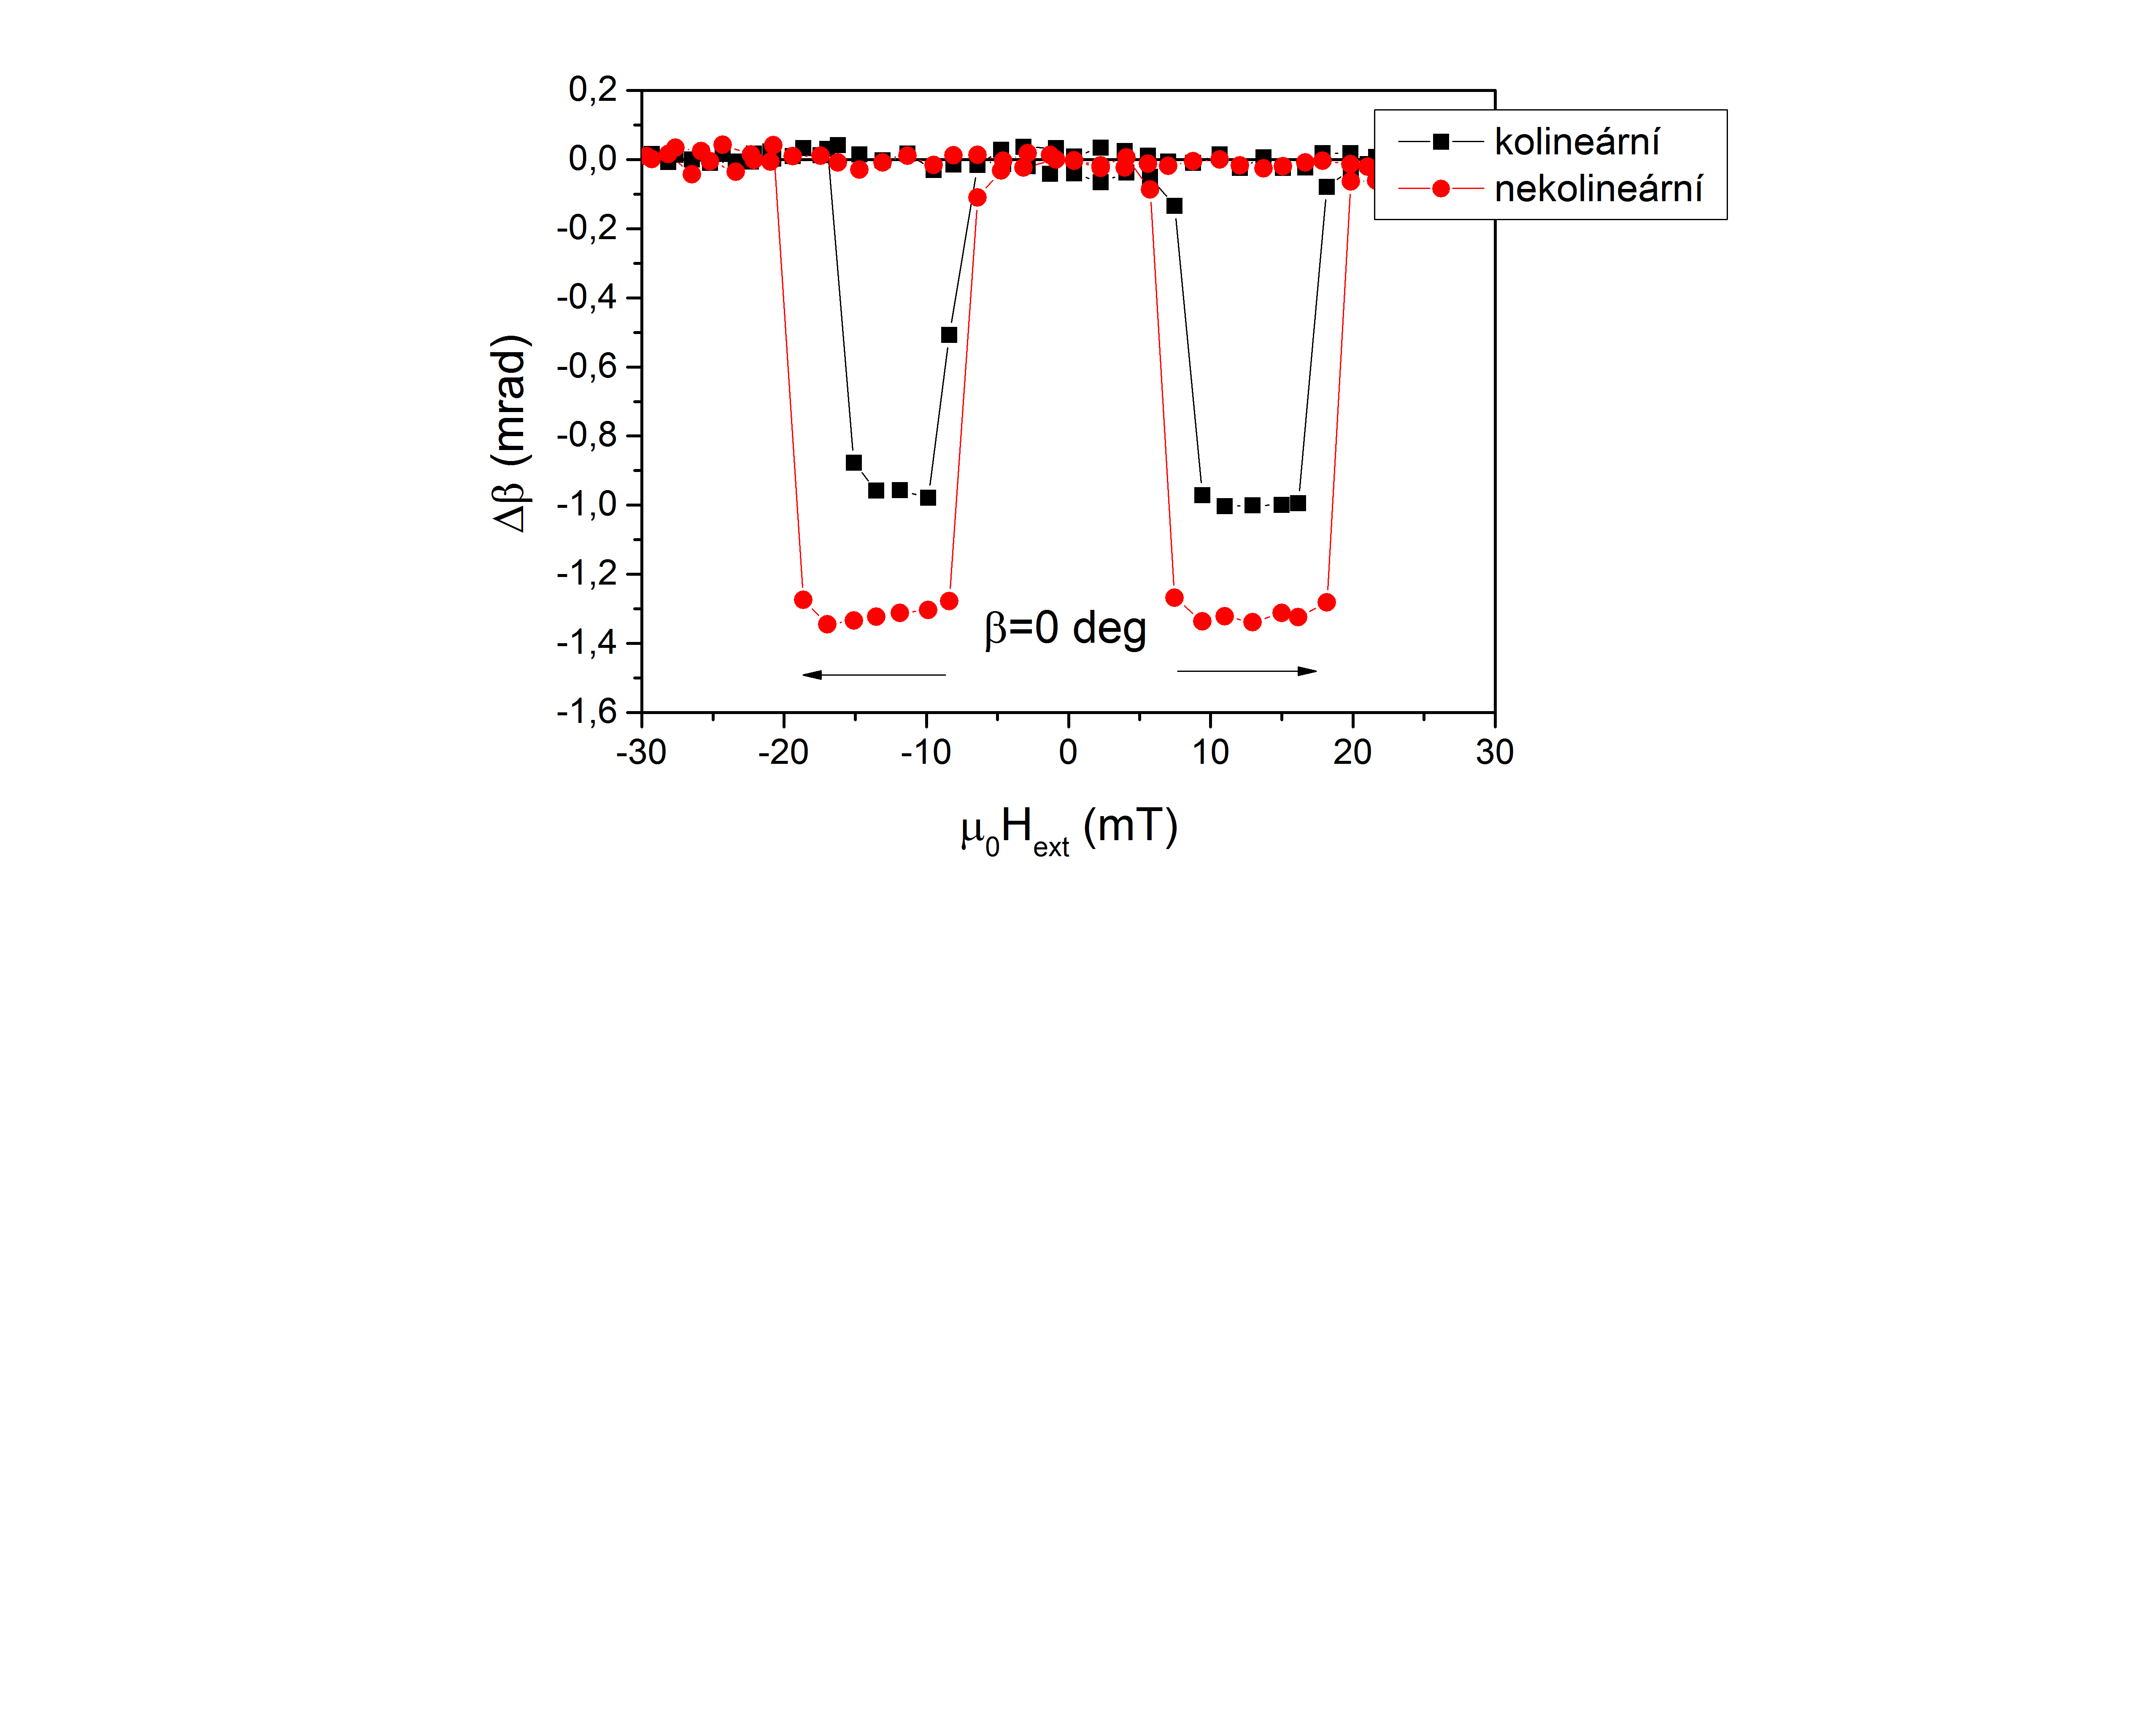
\includegraphics[trim={0 3.43in 0 0}, clip, width=\textwidth]{./png/kolhyst_nekol}}
	\caption{Porovnání Voigtova jevu v kolineární a nekolineární geometrii. Měření v kolineární geometrii pravděpodobně proběhla při vyšší teplotě.}\label{kol_nekol}
\end{figure}


\subsection{Závislost na směru vnějšího pole} \label{kap_smer}

Měřili jsme hysterezní smyčky ve všech směrech pole s krokem \ang{15}. Ovládání elektromagnetu má v současné době implementované a zkalibrované pouze čtyři směry: \ang{0}, \ang{45}, \ang{90}, \ang{135}. Zbývajících směrů jsme dosáhli otočením ramena kryostatu se vzorkem o $+\ang{15}$ a $-\ang{15}$. Zároveň se vzorkem jsme točili i rovinu polarizace, aby byla splněna podmínka $\gamma-\beta=\ang{90}$ a Voigtův jev byl maximální.
Směry $\phH>\ang{165}$ jsme měřili jako \emph{down} opačného směru.

Měření proběhlo při teplotě $T<\SI{15}{\kelvin}$ a intenzita laseru dopadajícího na vzorek byla \SI{1,2}{\milli\watt}.

U hysterezních smyček sledujeme veličiny $\hcj$, $\hcd$ a $A$ (viz obr. \ref{kol_okolo}).
Ve směrech \ang{45}, \ang{60}, \ang{225}, \ang{240} jsme nepozorovali žádný magnetooptický signál, protože magnetizace v průběhu hysterezní smyčky zjevně přeskakuje pouze mezi dvěma protilehlými snadnými osami. To je v souladu s očekávanou polohou prvnní snadné osy v tomto vzorku (viz tabulka \ref{tab_vzorek}), která při zvoleném nalepení (viz obr. \ref{souradna_soustava_vzorek}) odpovídá směru $59(5)^\circ$. Překvapivý je ale fakt, že při položení pole ve směru druhé snadné osy, který by se měla nacházet na poloze $121(5)^\circ$, smyčky pozorujeme.

\begin{figure}[htbp]\centering
\qq{	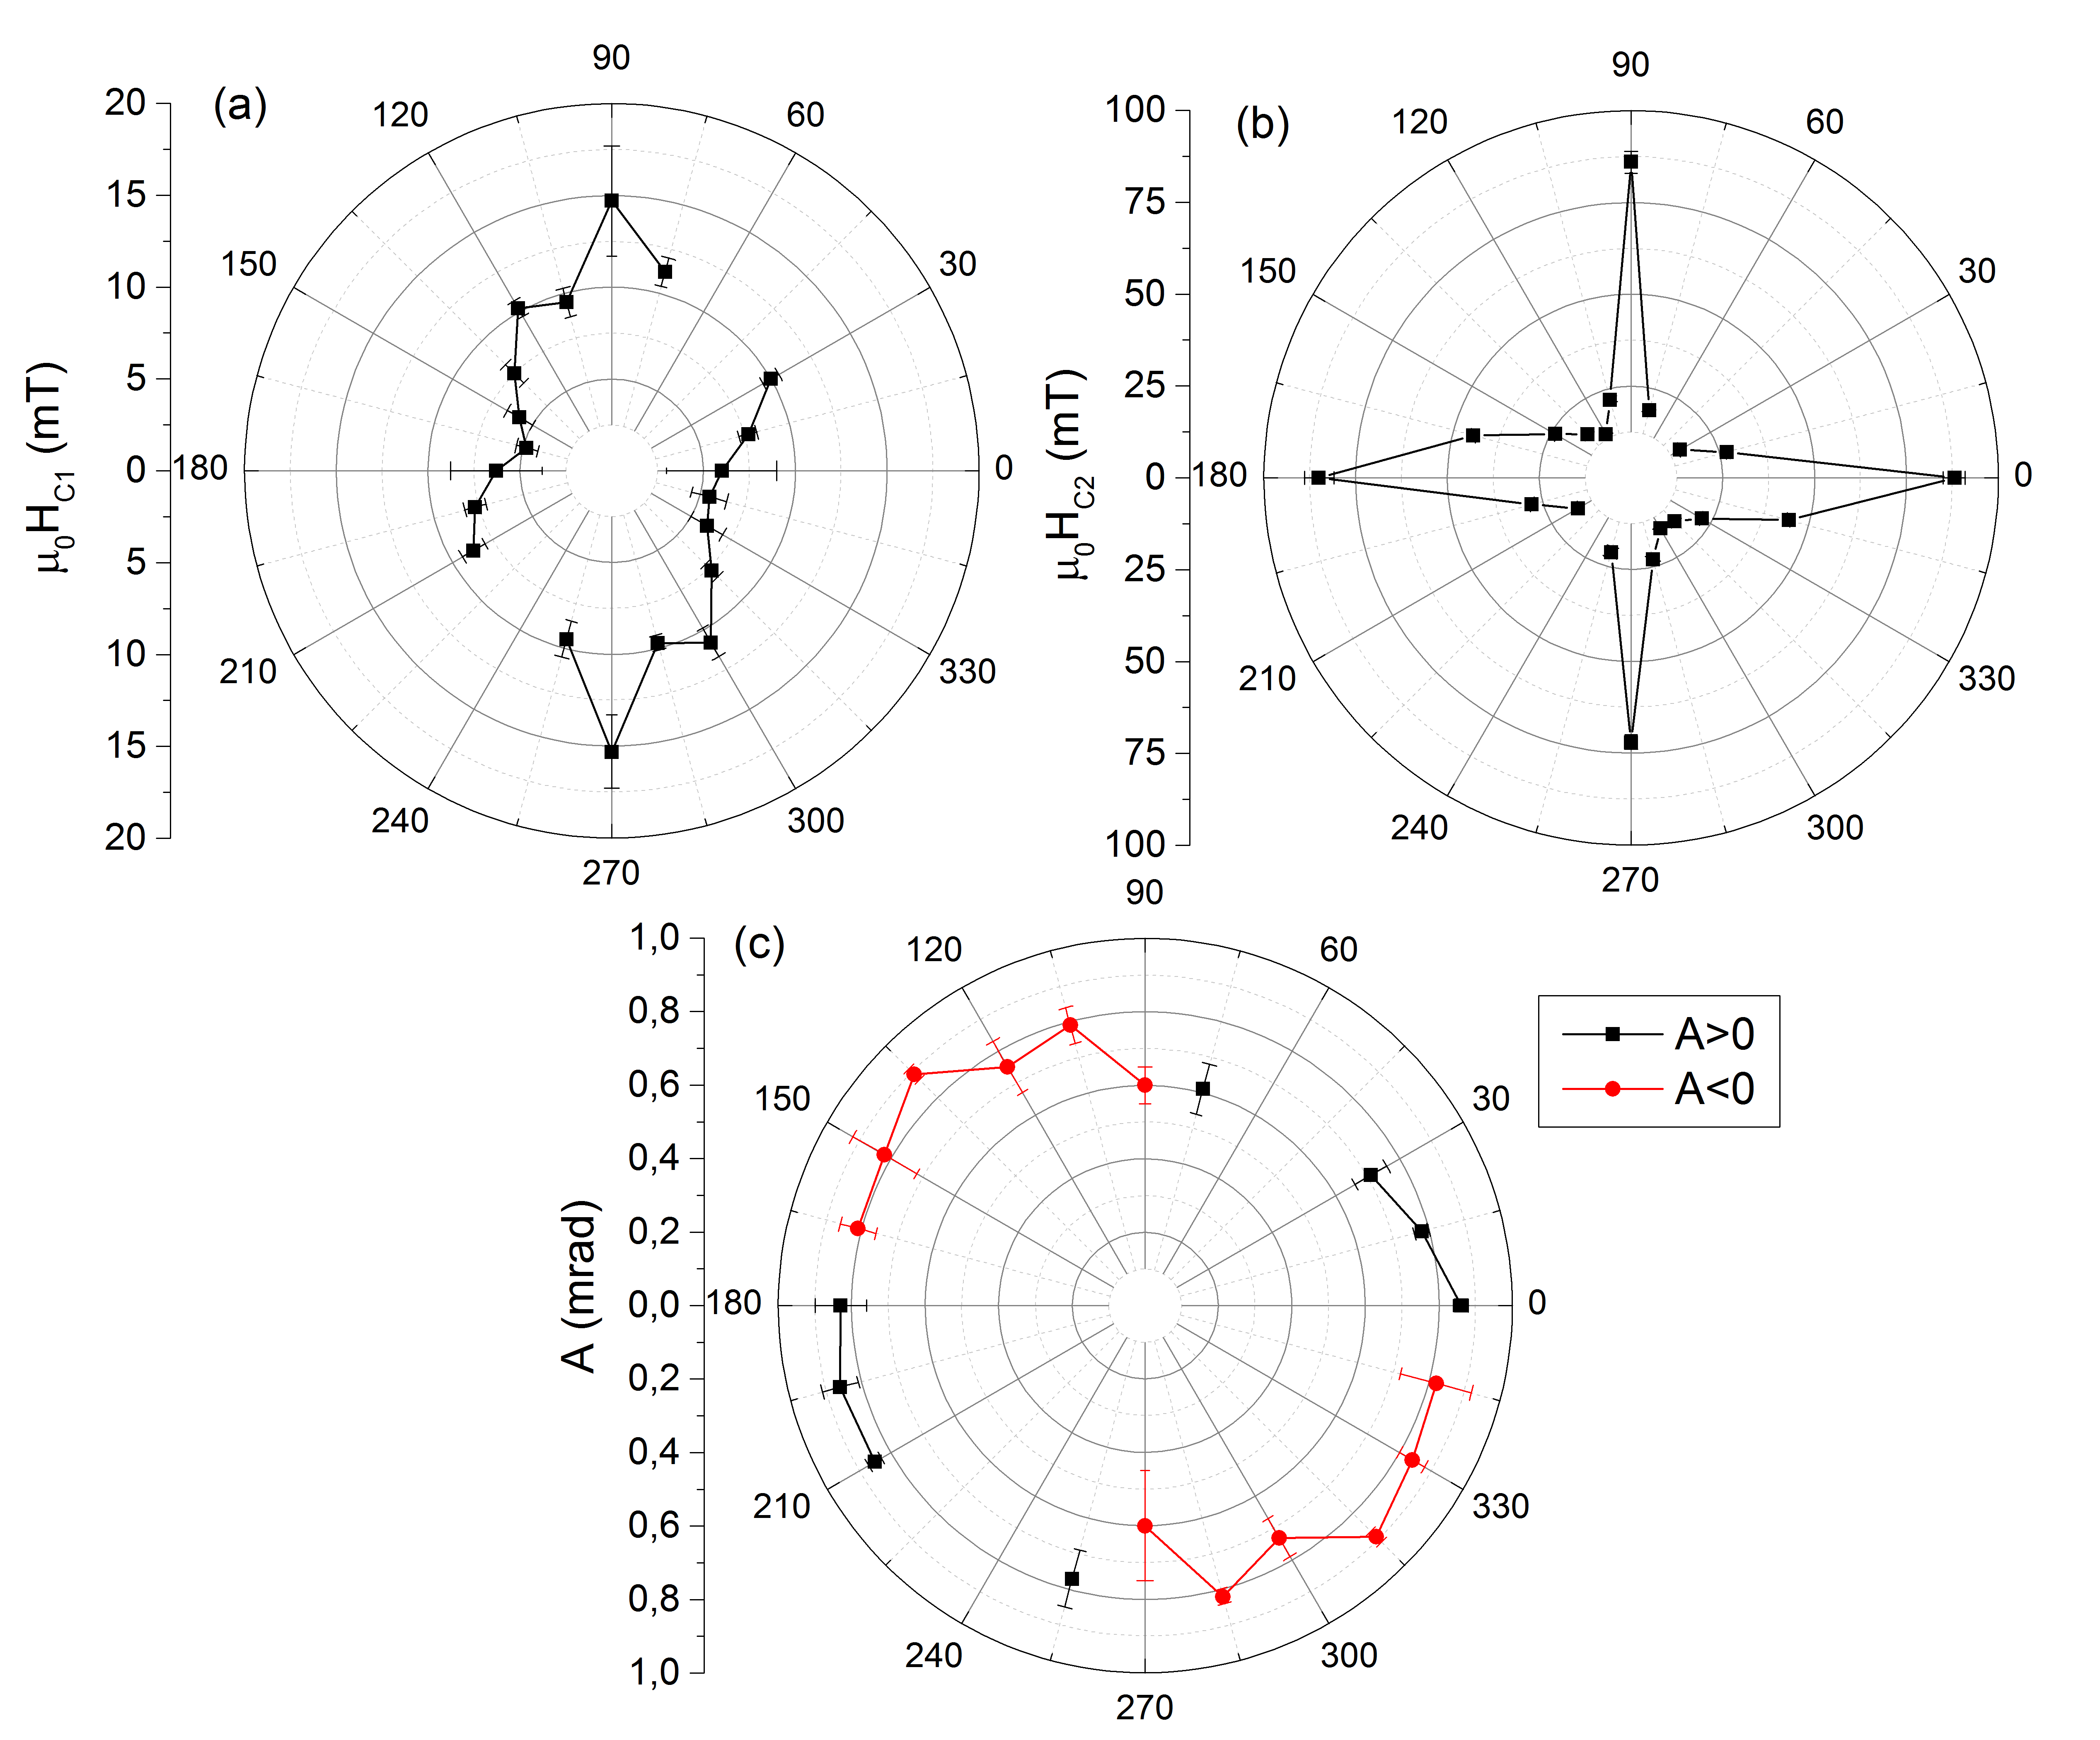
\includegraphics[width=\textwidth]{./png/hystgraf_okolo}}
	\caption{Měření Voigtova jevu v hysterezních smyčkách pro různá $\phH$. (a) Úhlová závislost $\hcj$. (b) Úhlová závislost $\hcd$. (c) Úhlová závislost amplitudy přeskoku $A$. Kladné hodnoty černě, záporné červeně.}\label{kol_okolo}
\end{figure}

Nejzajímavější je graf koercitivních polí $\hcd$, ve kterém jsou jasně patrné významné krystalografické směry [110] a [-110] (porovnejte s \ref{souradna_soustava_vzorek} (b)).



\subsection{Teplotní závislost při vnějším poli ve směru \ang{135}}

Vzorek jsme nejprve zchladili při vypnutém topení ($T=\SI{12(3)}{\kelvin}$). Nastavením teploty na termočlánku jsme vzorek zahřívali s krokem \SI{5}{\kelvin} až do takové teploty, kdy hysterezní smyčky přestaly být patrné. Skutečný rozsah měřených teplot byl 12-\SI{60}{\kelvin}. Intenzita laseru dopadajícího na vzorek byla \SI{2}{\milli\watt}.

Měříme pouze polarizaci $\beta=\ang{0}$, tedy $\gamma-\beta=\ang{90}$.

Teplotní závislost hysterezních smyček je na obr. \ref{kol_vysl_tep_voigt} (a). U hysterezních smyček sledujeme opět veličiny $\hcj$, $\hcd$ a $A$ (viz obr. \ref{kol_vysl_tep_voigt} (b), (c)).


\begin{figure}[htbp]\centering
\qq{	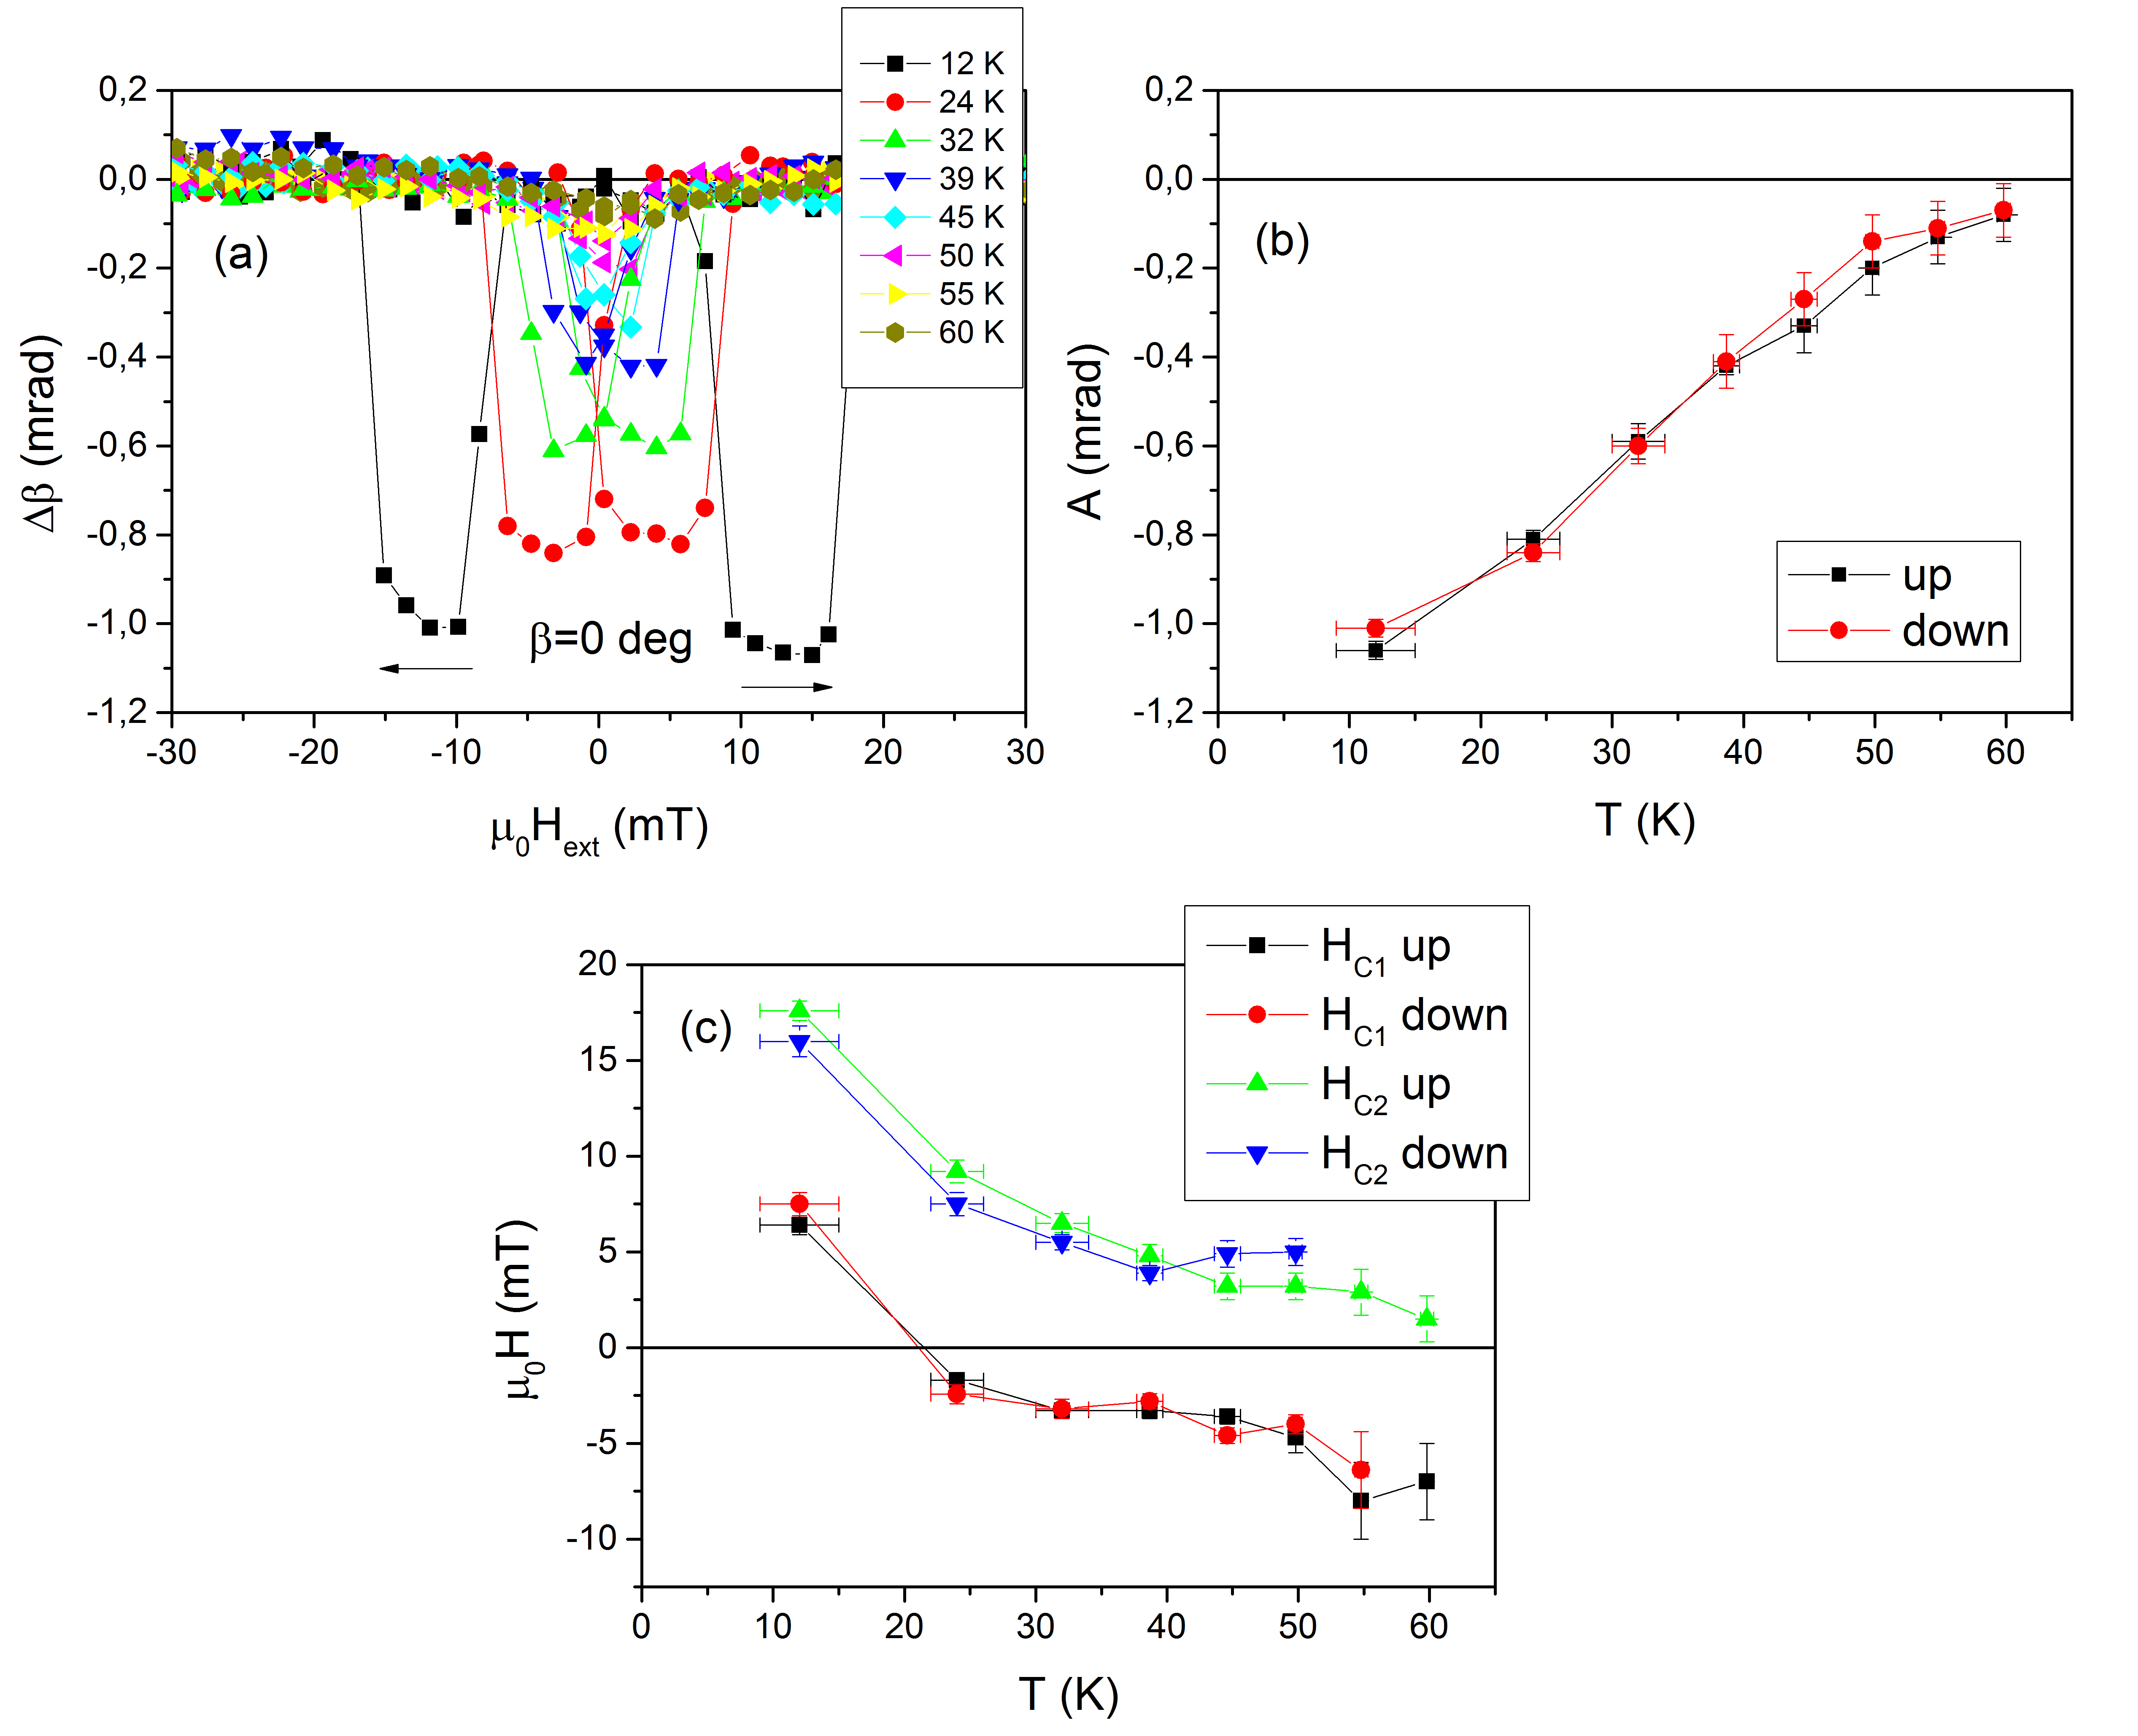
\includegraphics[width=\textwidth]{./png/kolhyst_135tepl}}
	\caption{Měření teplotní závislosti Voigtova jevu v hysterezních smyčkách pro $\phH=\ang{135}$ v kolineární geometrii. (a) Hysterezní smyčky při všech měřených teplotách. (b) Teplotní závislost amplitudy přeskoku $A$. (c) Teplotní závislost koercitivních polí.}\label{kol_vysl_tep_voigt}
\end{figure}

\chapter{Změna směru pole při jeho konstantní velikosti} \label{kap_toceni}

V této kapitole vyzkoušíme nový typ magnetooptického měření, který plně využívá výhody dvoudimenzionality elektromagnetu. Elektromagnet umožňuje při konstantní velikosti pole $\mu_0 \hext=\SI{50}{\milli\tesla}$, nebo \SI{210}{\milli\tesla} plynule měnit směr pole od $\phH=\ang{270}$ po směru hodinových ručiček do \ang{-90}, tedy plný rozsah úhlů. V~případě prokázání užitečnosti této metody je možné principiálně zkalibrovat a implementovat i jiné velikosti $\hext$, rozsahy úhlů a smysl otáčení pole (proti směru hodinových ručiček).

Provedli jsme tři měření tohoto druhu
\begin{itemize}
	\item $\mu_0 \hext=\SI{210}{\milli\tesla}$, $T<\SI{15}{\kelvin}$
	\item $\mu_0 \hext=\SI{50}{\milli\tesla}$, $T<\SI{15}{\kelvin}$
	\item $\mu_0 \hext=\SI{210}{\milli\tesla}$, $T=\SI{38,7(10)}{\kelvin}$
\end{itemize}
První dvě uvedená měření proběhla ve stejný den při stejném zchlazení vzorku.

Měření proběhlo v kolineární geometrii a intenzita laseru dopadajícího na vzorek byla \SI{1,2}{\milli\watt}.



\section{Teoretický popis}
Pomocí optického můstku změříme při daném průběhu pole klasicky rozdílový a součtový signál. Toto provedeme pro více polarizací $\beta \in (\ang{0}, \ang{180})$ s krokem \ang{15}.

Teď bychom rozdílový a součtový signál rádi převedli na veličiny $\Delta \beta$ a $B$ podobně jako v hysterezních smyčkách, ale narážíme na problém. V našem experimentu potřebujeme správně určit hladinu $\Delta \beta=0$, tzn. vyvážit můstek tak, aby nulové rozdílové napětí odpovídalo situaci, kdy dopadající a odražené světlo je lineárně polarizované ve stejné rovině. S veličinou $B$ narážíme na stejný nedostatek. 

Nabízí se možnost jako nulovou hladinu zvolit střední hodnotu každé křivky. Střední hodnotu ale počítáme vzhledem k $\phH$ a ne $\phM$, a proto nemusí být nutně nulová.
V každém bodě změřené křivky má magnetizace určitý definovaný směr a tedy existuje zatím neznámá funkční závislost $\phM(\phH)$. Podle \eqref{rotace_polarizace} platí
\begin{equation}
\Delta \beta(\phH, \beta) = \pmld \sin \left[ 2(\phM(\phH)-\beta) \right] \,.
\end{equation}
Střední hodnota naměřené křivky vzhledem k $\phH$ je tedy
\begin{equation}
\begin{aligned}
\str{\Delta\beta} &= \str{\pmld \sin \left[ 2(\phM-\beta) \right]} \\
&= \str{\pmld \sin(2\phM)\cos(2\beta)-\cos(2\phM)\sin(2\beta)} \\
&=  \str{\pmld\sin(2\phM)}\cos(2\beta)- \str{\pmld\cos(2\phM)}\sin(2\beta) \\
&=K \sin\left[ 2(\alpha-\beta) \right] \,, \\
\end{aligned}
\end{equation}
kde uvažujeme, že $\pmld$ může záviset na směru magnetizace a tím pádem i směru vnějšího pole. Označili jsme
\begin{equation}
\begin{aligned}
K&=\sqrt{ \str{\pmld\sin(2\phM) }^2 +  \str{\pmld\cos(2\phM) }^2 } \\
\tan(2\alpha) &=\frac{\str{\pmld\sin(2\phM) }}{\str{\pmld\cos(2\phM) }}
\end{aligned}
\end{equation}

Pokud zvolíme jako nulovou hladinu $\Delta\beta$ její střední hodnotu, dostaneme veličinu, pro kterou platí
\begin{equation}
\left[ \Delta \beta - \str{\Delta\beta}  \right](\phH, \beta)=\pmld \sin[2(\phM-\beta)] - K \sin\left[ 2(\alpha-\beta) \right] \,.
\end{equation}
$\phM(\phH)$ a $\pmld(\phM)$ jsou zatím neurčené hledané závislosti. $K$ a $\alpha$ jsou vzhledem k $\phH$ a $\beta$ konstanty, ale závisí na hledaných $\phM(\phH)$ a $\pmld(\phM)$ v celém rozsahu $\phH$.

Pokud změříme $m$ různých $\phH$ a $n$ různých $\beta$, budeme mít $mn$ hodnot a $2m$ neznámých parametrů $\phM$ a $\pmld$, které by principiálně bylo možné nafitovat. Jednalo by se ovšem o obrovský nelineární fit a výsledky navíc nemusí být jednoznačné.
Výpočetně snazší možností by byla selfkonzistentní metoda. V této práci zatím používáme zjednodušený model.

Vzorek, se kterým pracujeme, má přibližně kubickou symetrii (viz kapitola \ref{kap_vzorek}), tj. je přibližně symetrický při otočení o \ang{90} v rovině $xy$. Je-li tomu tak, pak vymizí konstanta $K$ a platí
\begin{equation} \label{e:asass}
\left[ \Delta \beta - \str{\Delta\beta}  \right](\phH, \beta)=\pmld \sin[2(\phM-\beta)] \,,
\end{equation}
což nám umožňuje fitovat pouze $\phM$ a $\pmld$ v řezech $\phH=\text{konst}$.

Podobně pro $B$
\begin{equation} \label{e:sss}
\left[ B - \str{B}  \right](\phH, \beta)=2\pmld \cos[2(\phM-\beta)] \,.
\end{equation}


\section{Metoda měření a zpracování dat}

Metoda měření i zpracování dat je ve všech třech měřených případech totožná. Čtenáře důkladně provedeme první sadou měření a u zbylých dvou uvedeme pouze výsledky.

Náš vzorek má téměř kubickou symetrii (viz tabulka \ref{tab_vzorek}) a proto použijeme výše uvedený postup.
Měříme vždy rozsah $\phH$ od \ang{270} do \ang{-90} s krokem \ang{5}.

Způsob zpracování dat z tohoto experimentu je oproti měření hysterezních smyček mnohem citlivější na šum (jednotlivé hodnoty změřených bodů i dlouhodobý drift). Proto každé jednotlivé měření provádíme pětkrát za sebou. Změřené křivky zprůměrujeme, tj. pro každé $\phH$ obdržíme hodnotu (rozdílové a součtové napětí) jako průměr z pěti hodnot, z každé změřené křivky jedna pro dané $\phH$.


Součtový a rozdílový signál přepočteme na $\Delta\beta$ a $B$ a od každé z křivek odečteme její střední hodnotu, jak je popsáno výše.
Príklad takových křivek je na obr. \ref{toc_hrube} (a), (b). 


\begin{figure}[htbp]\centering
\qq{	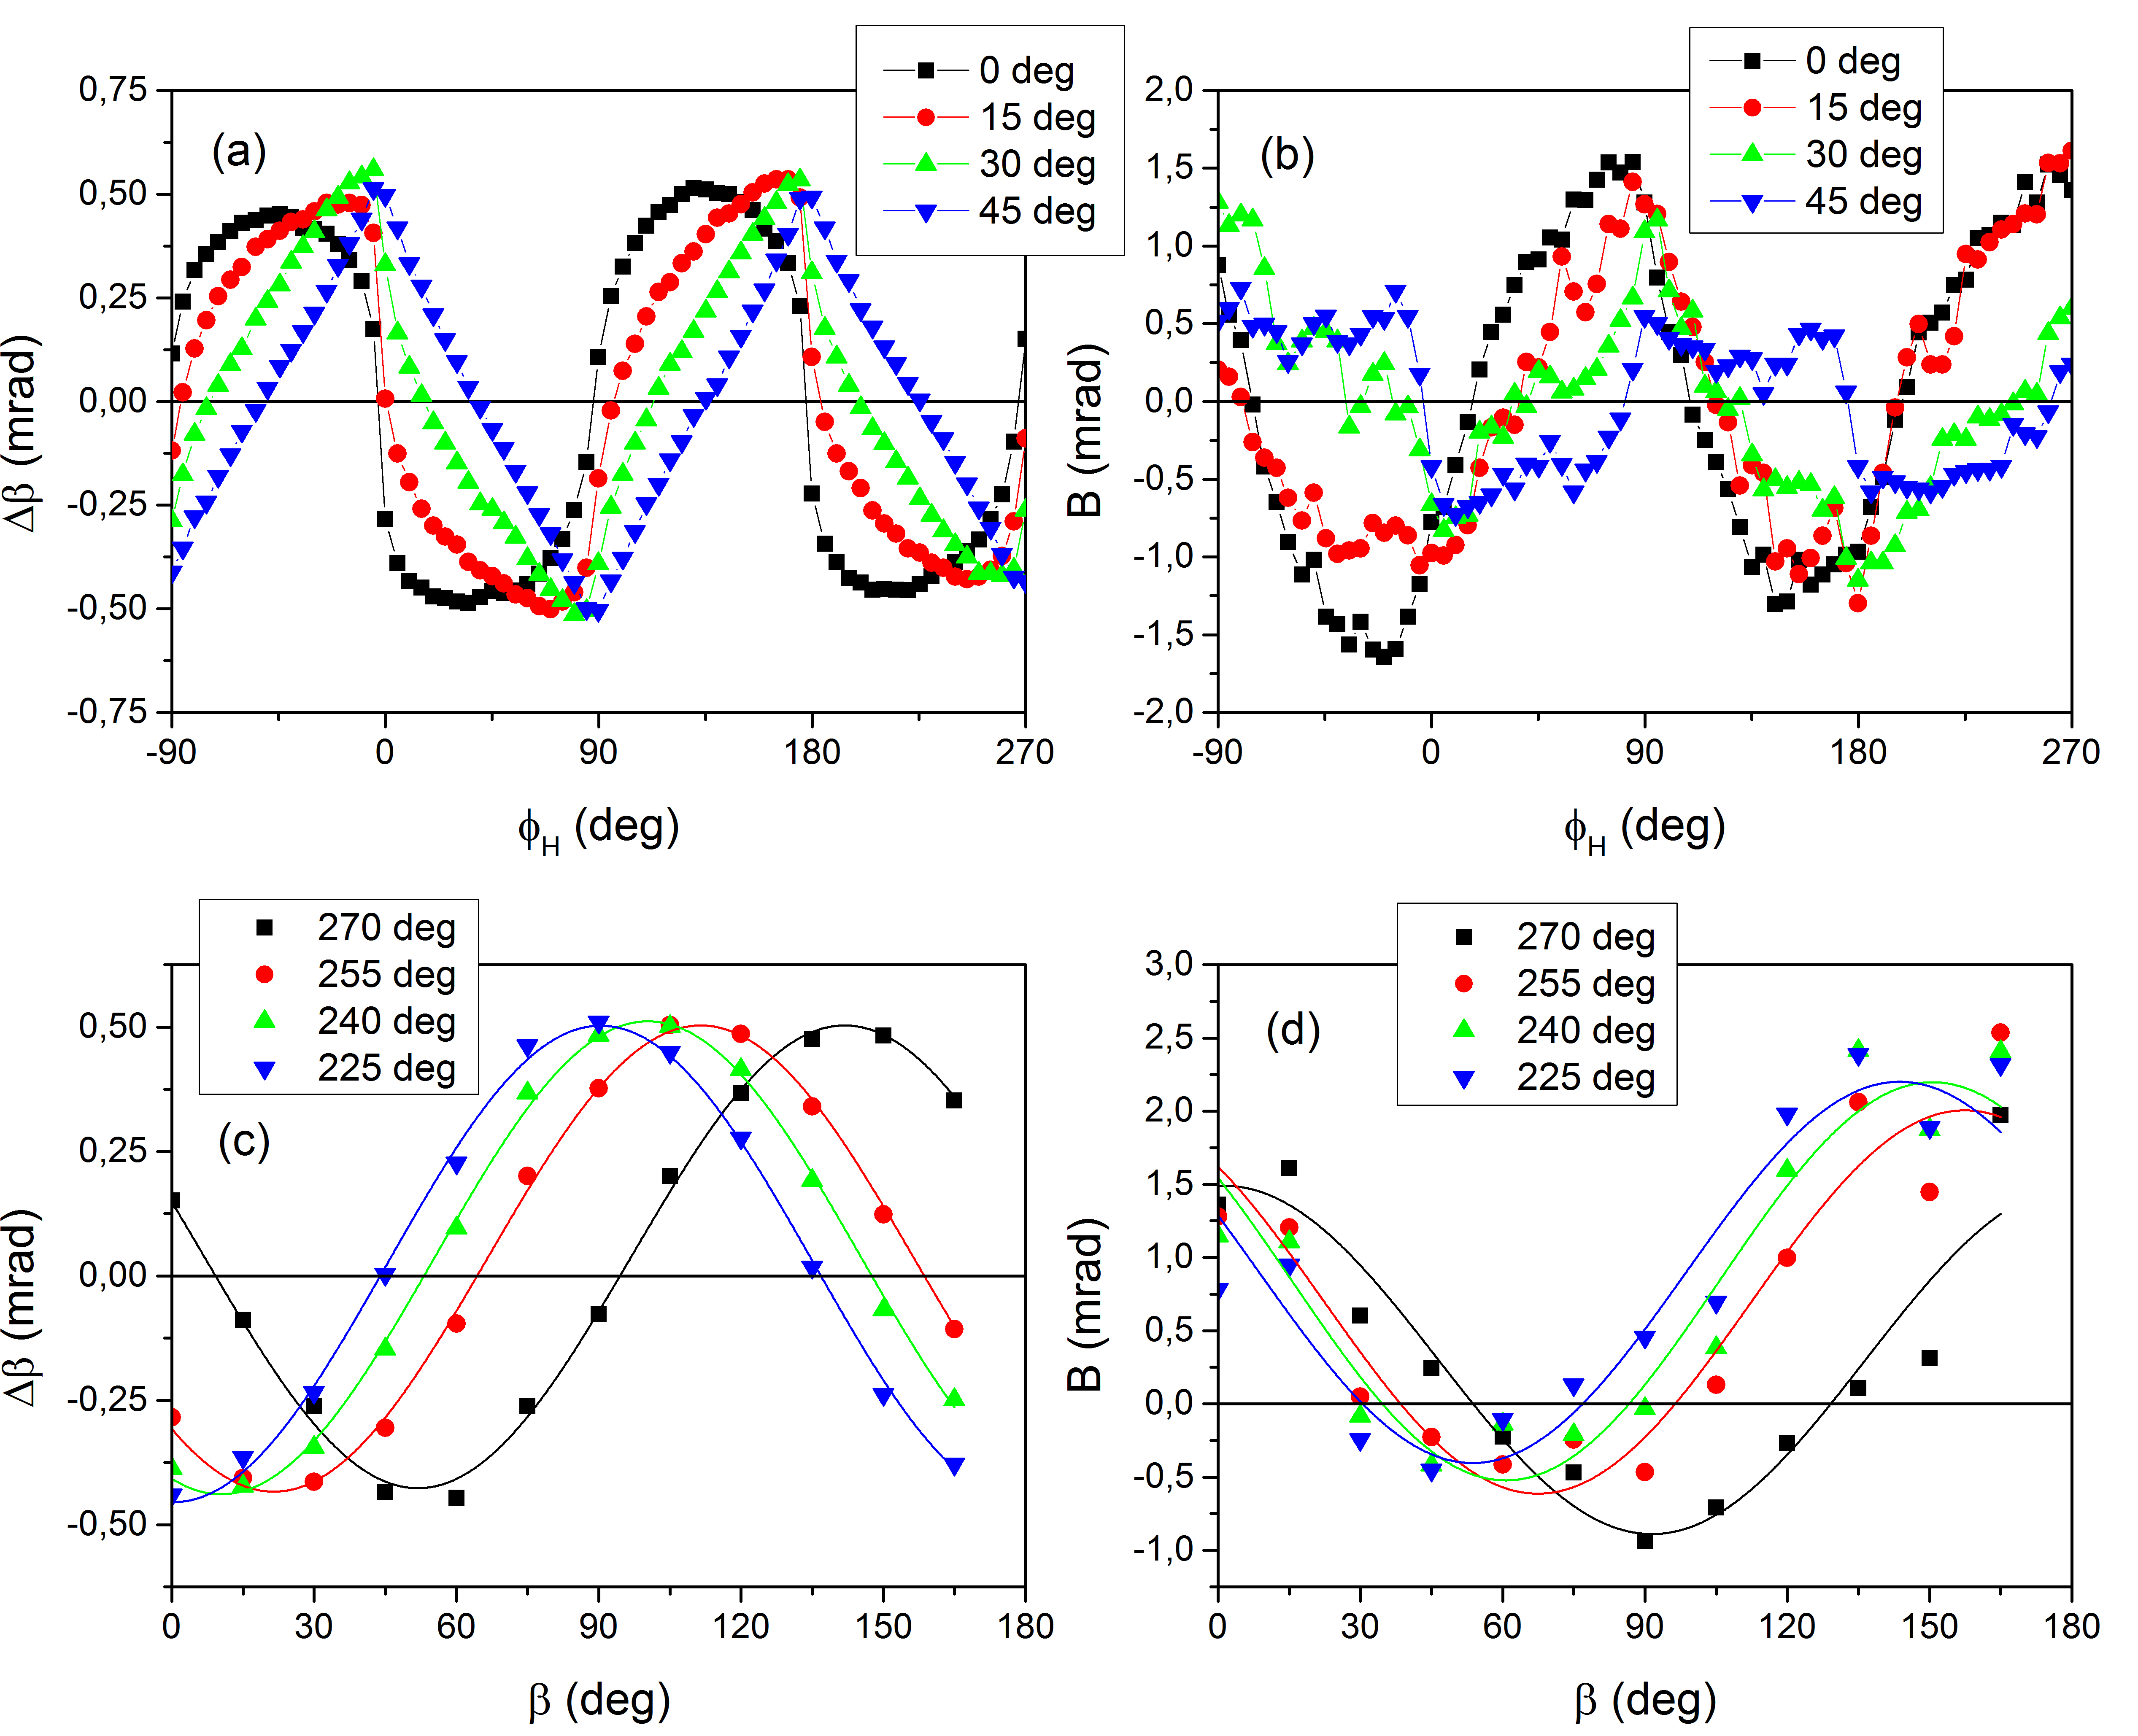
\includegraphics[width=\textwidth]{./png/graftoc_zpracovani}}
	\caption{Změna směru pole při jeho konstantní velikosti $\mu_0 \hext=\SI{210}{\milli\tesla}$ při $T<\SI{15}{\kelvin}$. (a) Voigtův jev pro vybrané polarizace. (b) MLD pro vybrané polarizace. (c) Přeskládaná data pro vybrané směry pole $\phH$ --- Voigtův jev, (d) MLD}\label{toc_hrube}
\end{figure}

Naměřená data mají nezávislou proměnnou $\phH$ a parametr $\beta$. Přeskládáme je tak, aby nezávislá proměnná byla $\beta$ a parametr $\phH$ jako na obr. \ref{toc_hrube} (c), (d).
Získané závislosti dále fitujeme funkcemi \eqref{e:asass} a \eqref{e:sss}. Poměrně často, především v $B$, však dochází k tomu, že závislost má zřetelně harmonický průběh, ale je posunutá (viz obr. \ref{toc_preskladane} (a)). Proto závislosti fitujeme také funkcemi s přidaným absolutním členem
\begin{equation} \label{e:tocsc}
\begin{aligned}
\Delta \beta(\phH, \beta) &= \pmld \sin \left[ 2(\phM(\phH)-\beta) \right]+c \,, \\
B(\phH, \beta) &= 2 \left(\pmld \cos \left[ 2(\phM(\phH)-\beta) \right]+c \right) \,.
\end{aligned}
\end{equation}
Výsledné $\phM$ a $\pmld$ z fitu s absolutním členem a bez jsou ve všech případech od sebe nerozeznatelné, pouze nejistota fitu je s absolutním členem mnohem menší.

\begin{figure}[htbp]\centering
\qq{	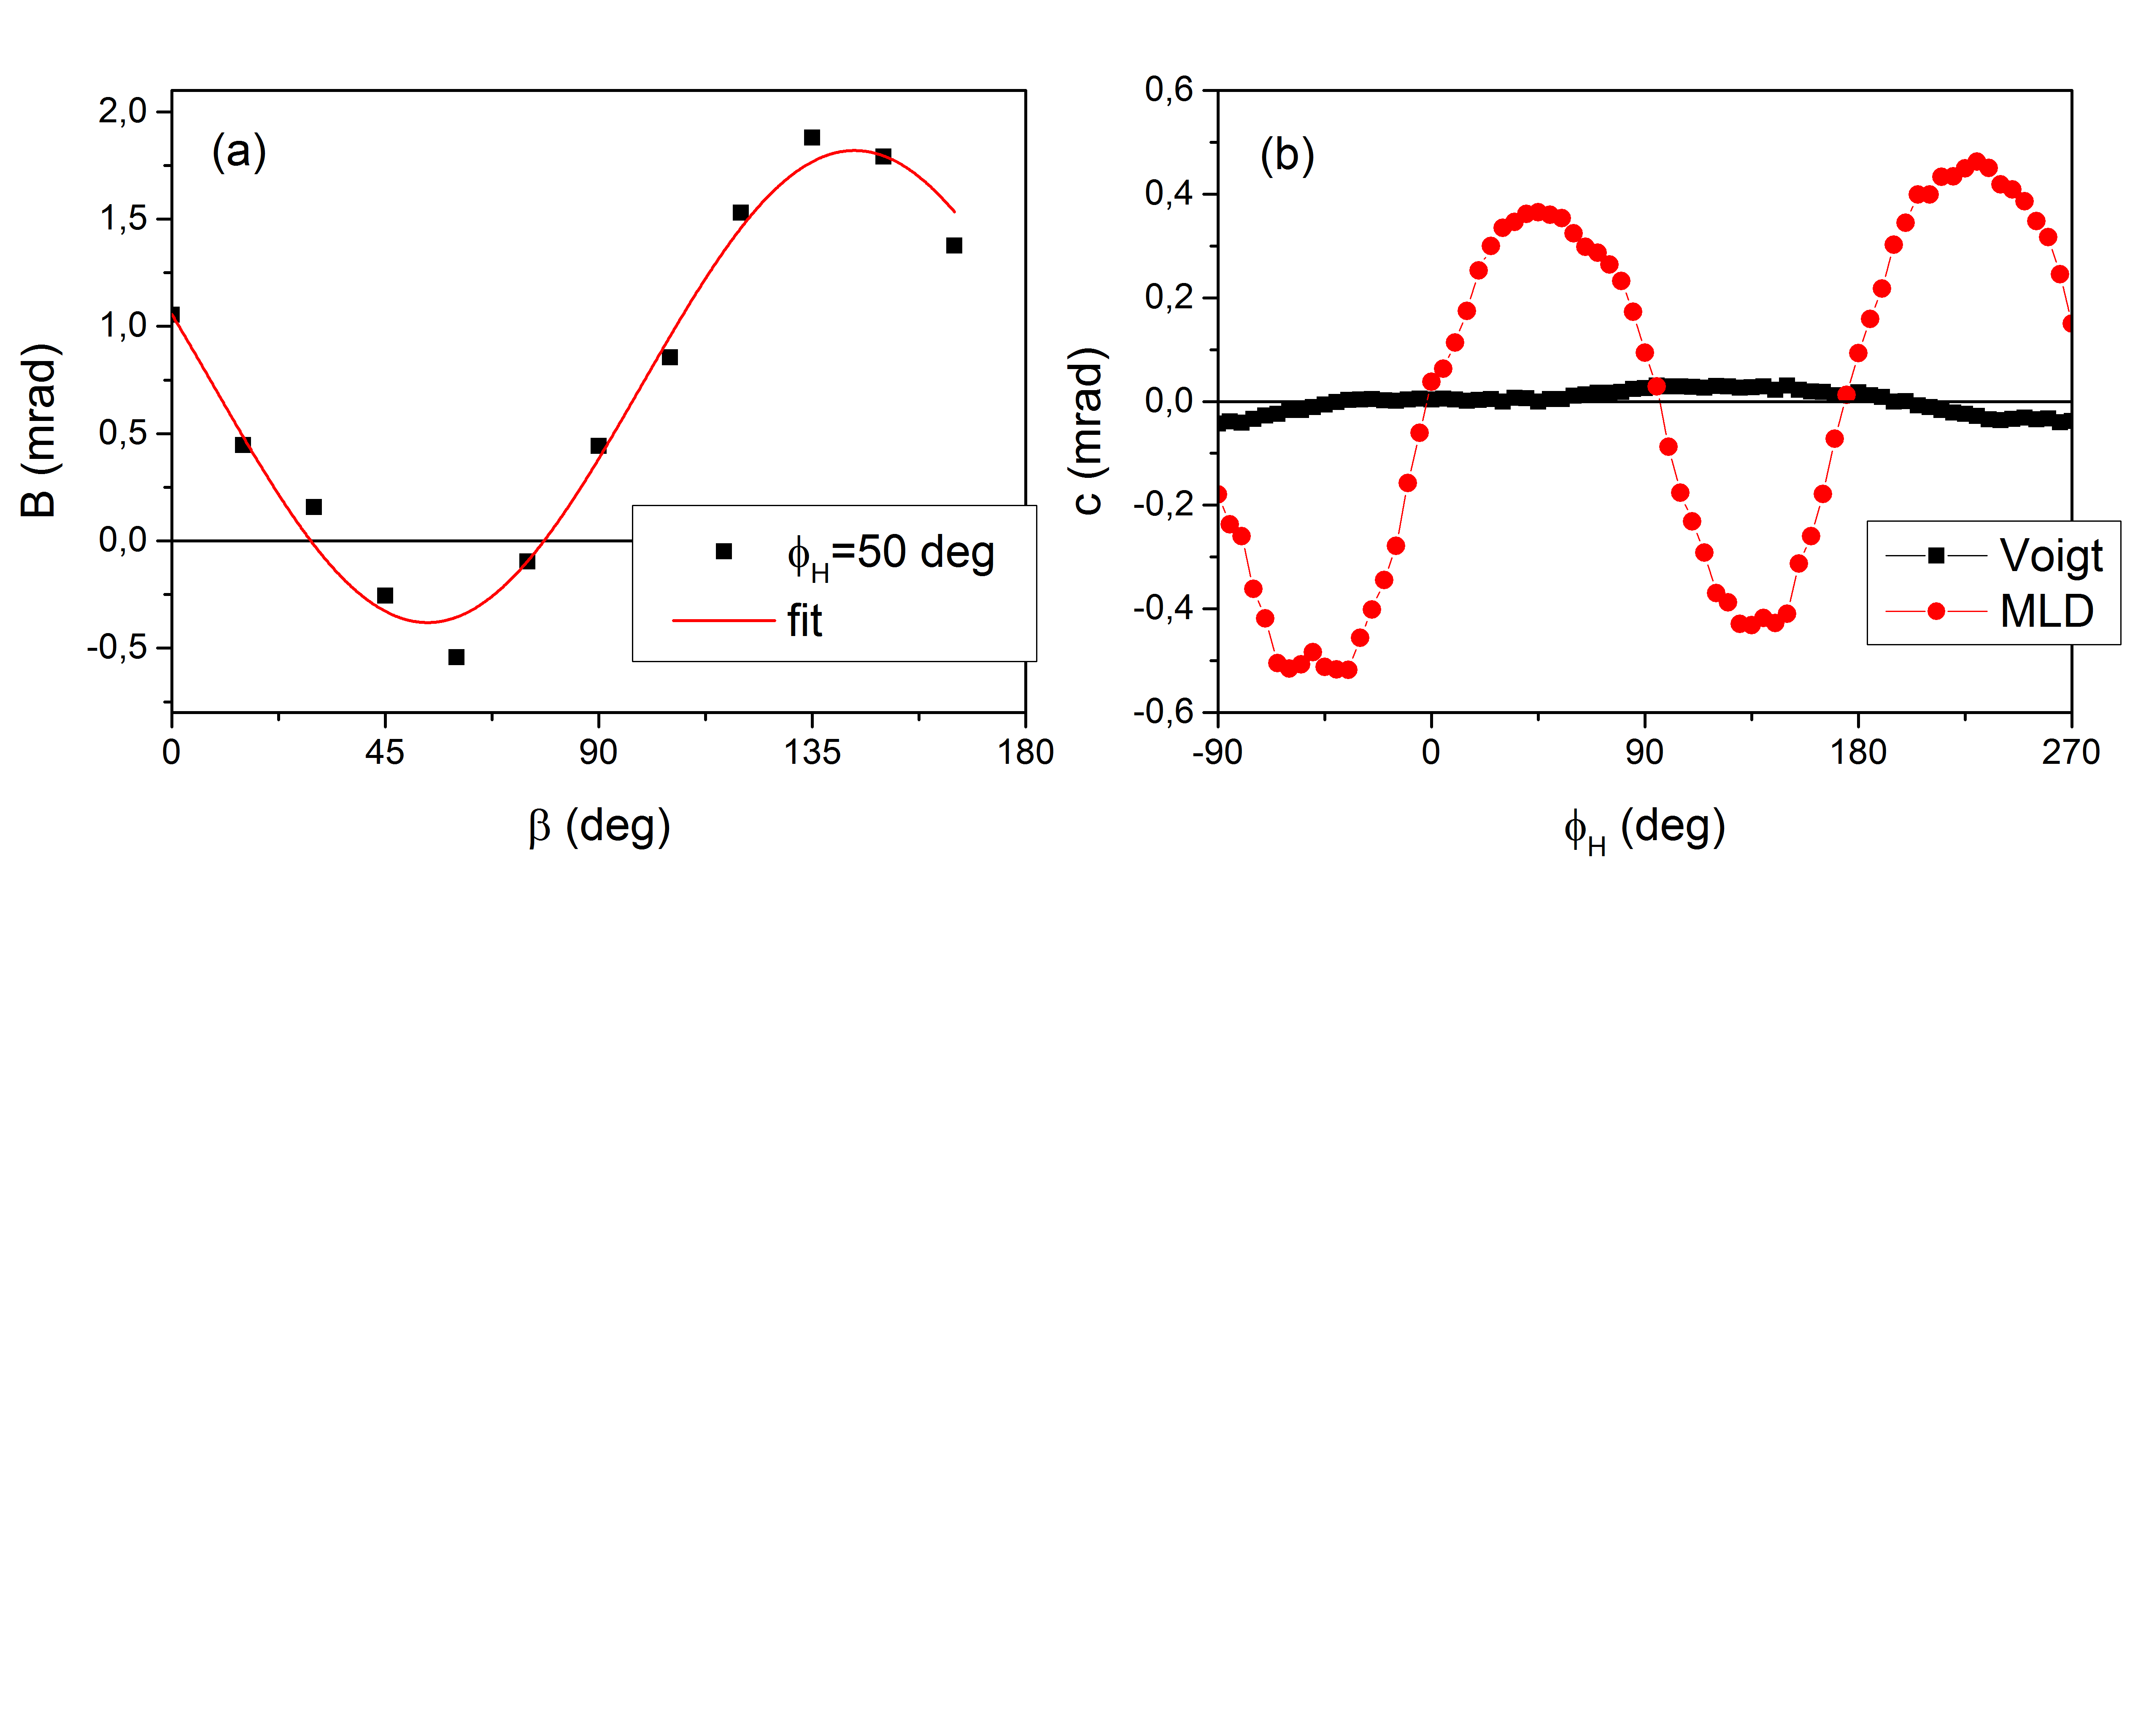
\includegraphics[trim={0 3.43in 0 0}, clip, width=\textwidth]{./png/graftoc_preskladane}}
	\caption{Změna směru pole při jeho konstantní velikosti $\mu_0 \hext=\SI{210}{\milli\tesla}$ při $T<\SI{15}{\kelvin}$. (a) Příklad přeskládaných dat s nenulovým absolutním členem. (b) Fitované absolutní členy $c$.}\label{toc_preskladane}
\end{figure}

\section{Výsledky}

Hlavními výsledky těchto experimentů jsou závislosti $\phM(\phH)$ a $\pmld(\phM)$.
Na obr. \ref{toc_vysledkyuhel} jsou grafy závislostí $\phM(\phH)$, pro každý směr pole je vynesena hodnota $\phM-\phH$, tj. úhel, který spolu svírá magnetizace a pole.

Pokud by pole bylo podstatně silnější než magnetická anizotropie ve vzorku, magnetizace by vždy mířila do směru pole a na grafu bychom pozorovali kružnici $\phM-\phH=\ang{0}$. Z grafu \ref{toc_vysledkyuhel} (a) je patrné, že při $T<\SI{15}{\kelvin}$ není tato podmínka splněna ani pro $\mu_0\hext=\SI{210}{\milli\tesla}$. Při $\hext=\SI{50}{\milli\tesla}$ (obr. \ref{toc_vysledkyuhel} (b)) je efekt ještě výraznější, v nespojitostech dochází k přeskoku mezi snadnými osami. Z~těchto změřených závislostí je možné jednoznačně určit polohu snadných os magnetizace ve vzorku (body $\phM=\phH$). Z obr. \ref{toc_vysledkyuhel} (b) můžeme tedy určit, že ve studovaném vzorku F002 se tyto osy nacházejí ve směrech $\num{45(5)}^\circ$ a $\num{136(5)}^\circ$, což vzhledem ke krystalografickému směru [100] (stejně jako v tabulce \ref{tab_vzorek}) odpovídá úhlům $\num{90(7)}^\circ$ a $\num{181(7)}^\circ$. Dříve provedená měření magnetické anizotropie v tomto vzorku, která byla uskutečněna pomocí laserovými pulzy vyvolané precese magnetizace \cite{TesarovaDisertace} vedla k závěru, že tyto snadné směry se nacházejí pro úhly $\num{104(5)}^\circ$ a $\num{166(5)}^\circ$ (viz tabulka \ref{tab_vzorek}). Tyto hodnoty se sice ani v rámci chyby měření neshodují, ale nejsou příliš odlišné. Je velice pravděpodobné, že jejich polohu umožňuje přesněji určit metoda popsaná v této práci.
Při vyšší teplotě (obr. \ref{toc_vysledkyuhel} (c)) se křivka mnohem více podobá kružnici. Dochází k měknutí anizotropie a magnetizace přesněji kopíruje směr pole.

Z grafů je též zřejmé, že měření pomocí Voigtova jevu je výrazně přesnější než MLD, což není překvapivé vzhledem k vyšší zašuměnosti součtového signálu (porovnejte \ref{toc_hrube} (a) a (b)).
Dále proto pro úhlovou závislost $\pmld(\phM)$ používáme pouze nafitované $\phM(\phH)$ z Voigtova jevu.
Hlavní výhoda měření i součtového signálu (MLD) je to, že nám umožňuje snadno určit znaménko $\pmld$.

Na obr. \ref{toc_vysledkypmld} (a) je úhlová závislost $\pmld(\phM)$ při $T<\SI{15}{\kelvin}$ při velikostech pole $\mu_0\hext=\SI{210}{\milli\tesla}$ a \SI{50}{\milli\tesla}. Obě velikosti pole dávají podle očekávání stejné $\pmld$. Při nižším poli procházel směr magnetizace menším rozsahem úhlů, a tak máme hodnoty jen pro směry v těsné blízkosti snadných os. V grafu je pro ilustraci též vyneseno nafitované $\pmld$ z MLD při $\mu_0\hext=\SI{210}{\milli\tesla}$. I v případě urční $\pmld$ vede měření Voigtova jevu k podstatně menší chybě než měření MLD.

Na obr. \ref{toc_vysledkypmld} (b) je opět graf úhlové závislosti $\pmld$, tentokrát pro $\mu_0\hext=\SI{210}{\milli\tesla}$ a dvě různé teploty: \SI{12(3)}{\kelvin} a \SI{38,7(10)}{\kelvin}. Při vyšší teplotě dochází vlivem nižší magnetizace ke snížení $|\pmld|$. V obou případech je zde ale jasně patrná směrová závislost $\pmld$: Největší hodnotu $\pmld$ dosahuje pro $\phM\approx \ang{0}$ (resp. \ang{180}), což odpovídá krystalografickému směru [110]. Nejmenší hodnoty jsou naopak pro $\phM\approx \ang{45}+n\cdot \ang{90}$, kde $n$ je celé číslo, což odpovídá krystalografickým směrům [100] a [010]. Tato měření tedy umožňují od sebe oddělit na krystalografickém směru závislé a nezávislé složky magnetooptického koeficientu $\pmld$.

\begin{figure}[htbp]\centering
\qq{	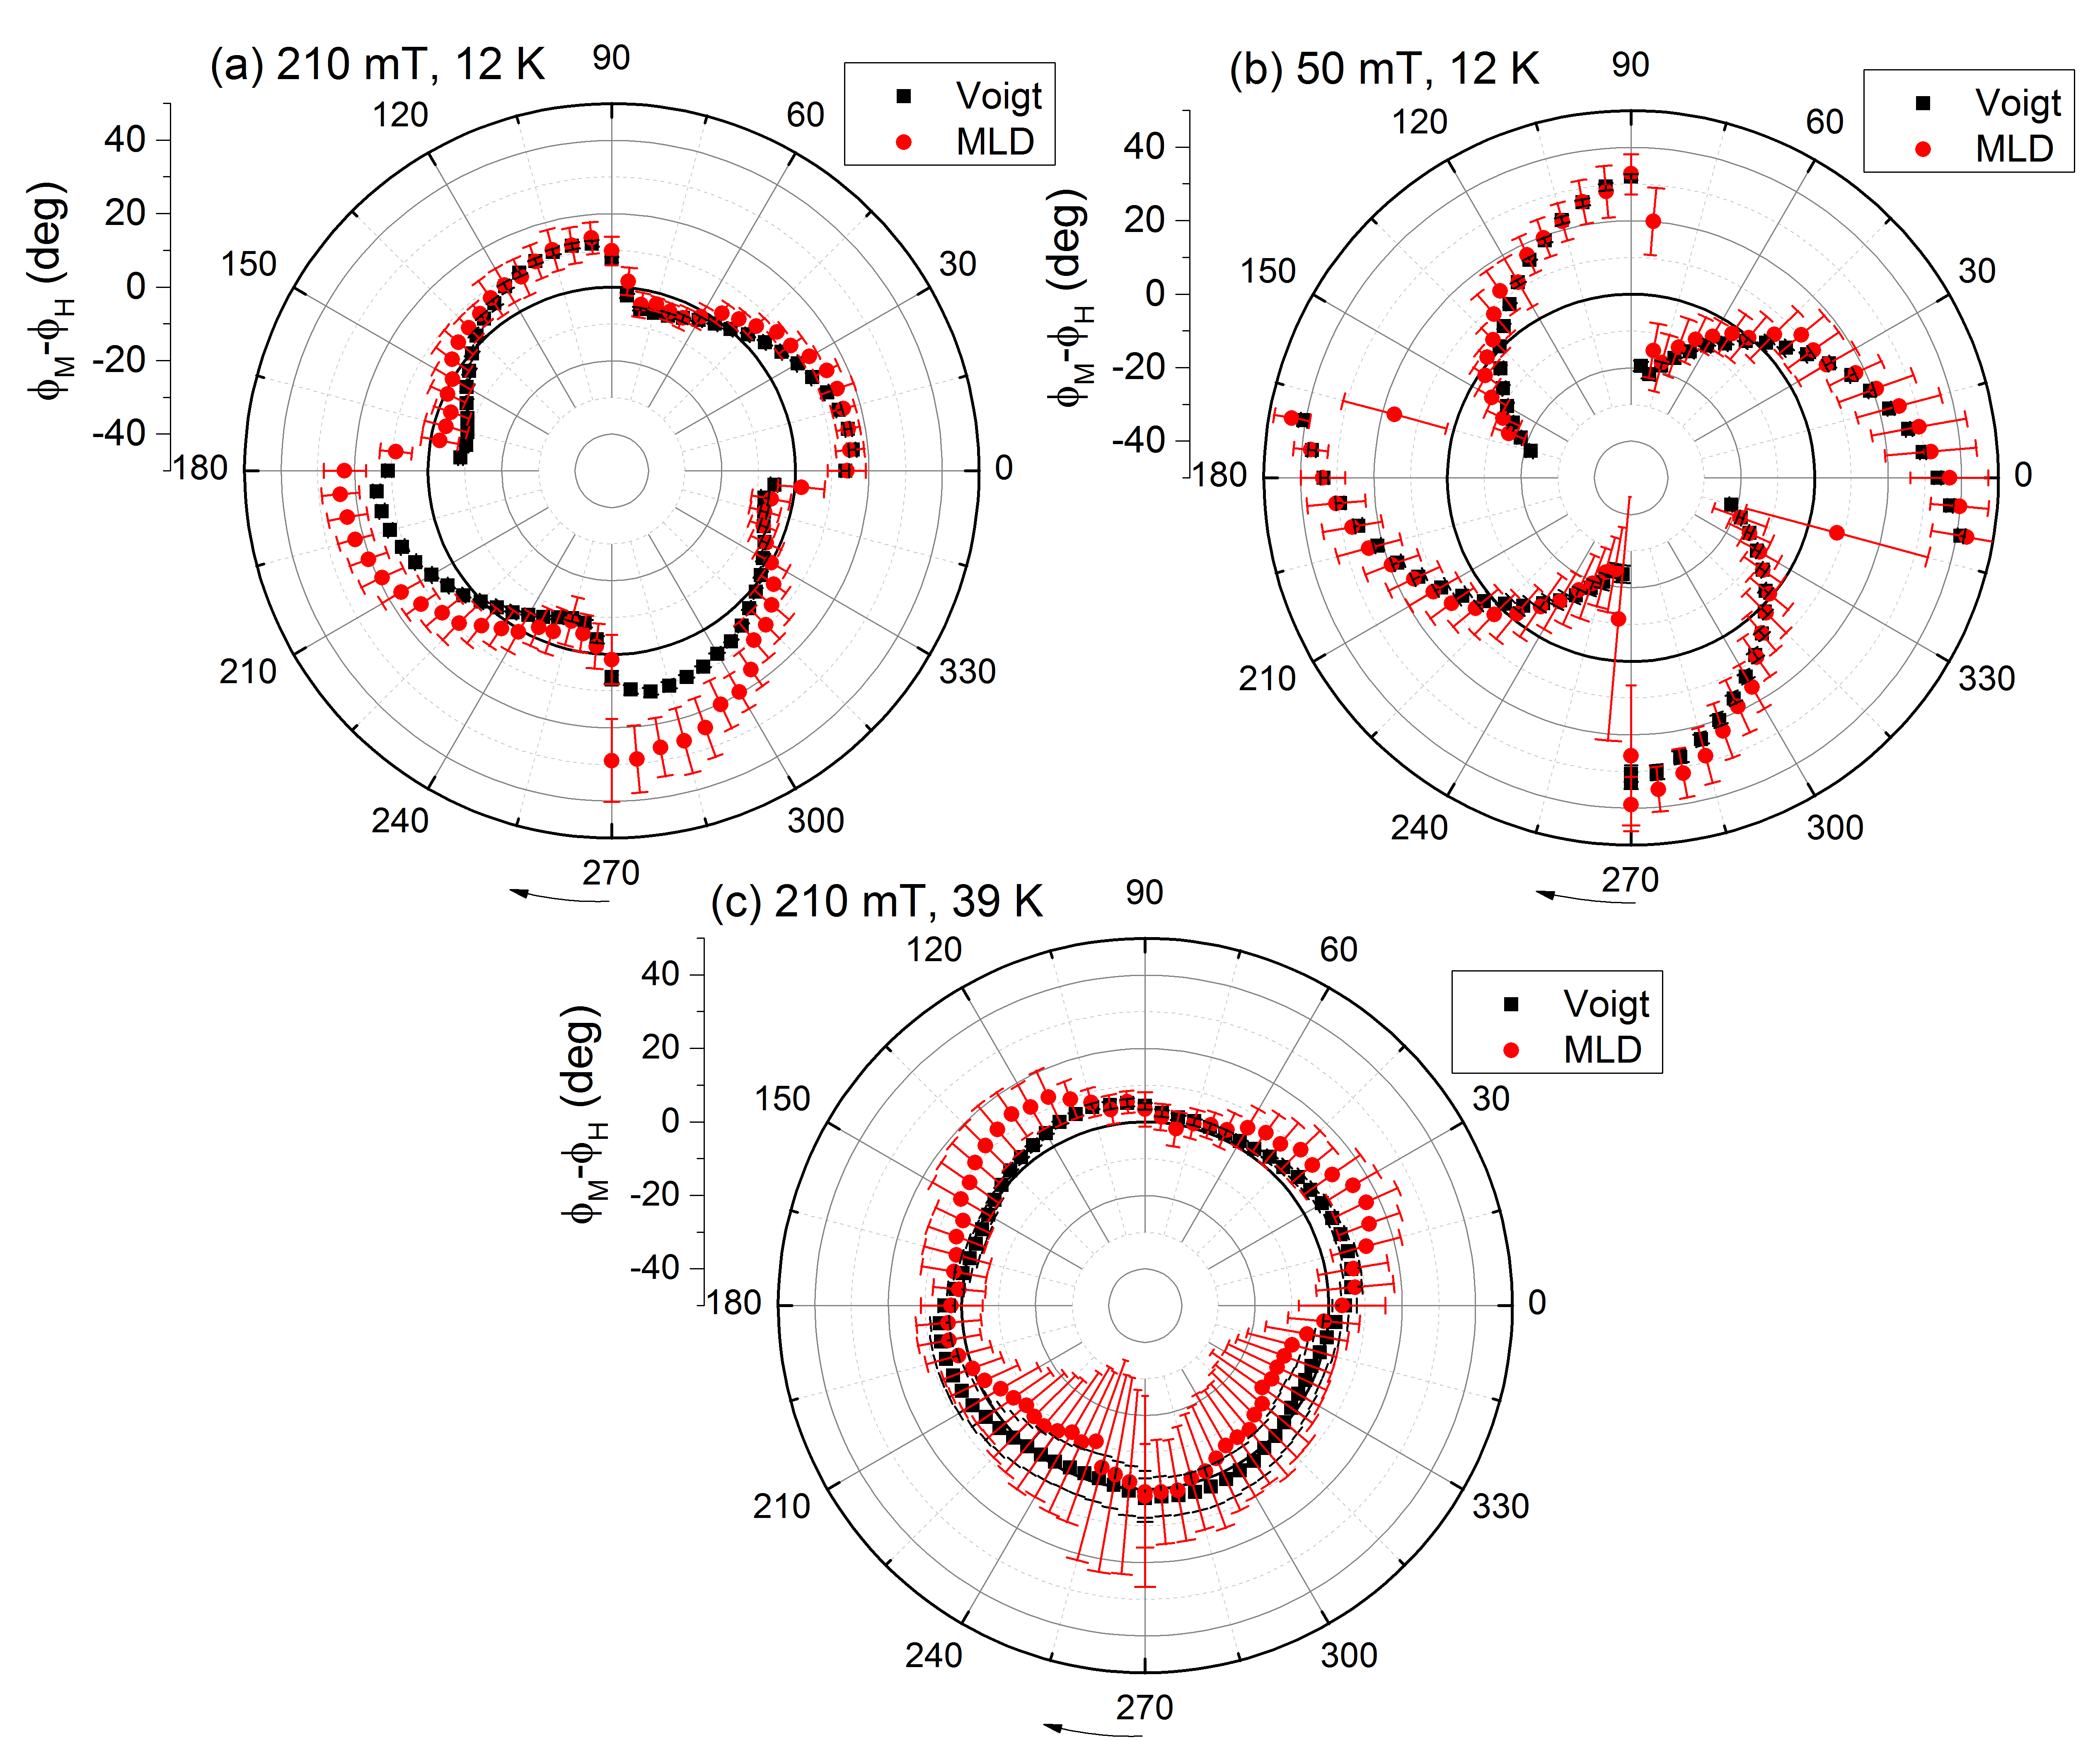
\includegraphics[width=\textwidth]{./png/tocgraf_uhly}}
	\caption{Změna směru pole při jeho konstantní velikosti. Závislost $\phM$ na směru vnějšího pole $\phH$. (a) $\hext=\SI{210}{\milli\tesla}$, $T<\SI{15}{\kelvin}$. (b) $\hext=\SI{50}{\milli\tesla}$, $T<\SI{15}{\kelvin}$. (c)  $\hext=\SI{210}{\milli\tesla}$, $T=\SI{38,7(10)}{\kelvin}$. }\label{toc_vysledkyuhel}
\end{figure}

\begin{figure}[htbp]\centering
\qq{	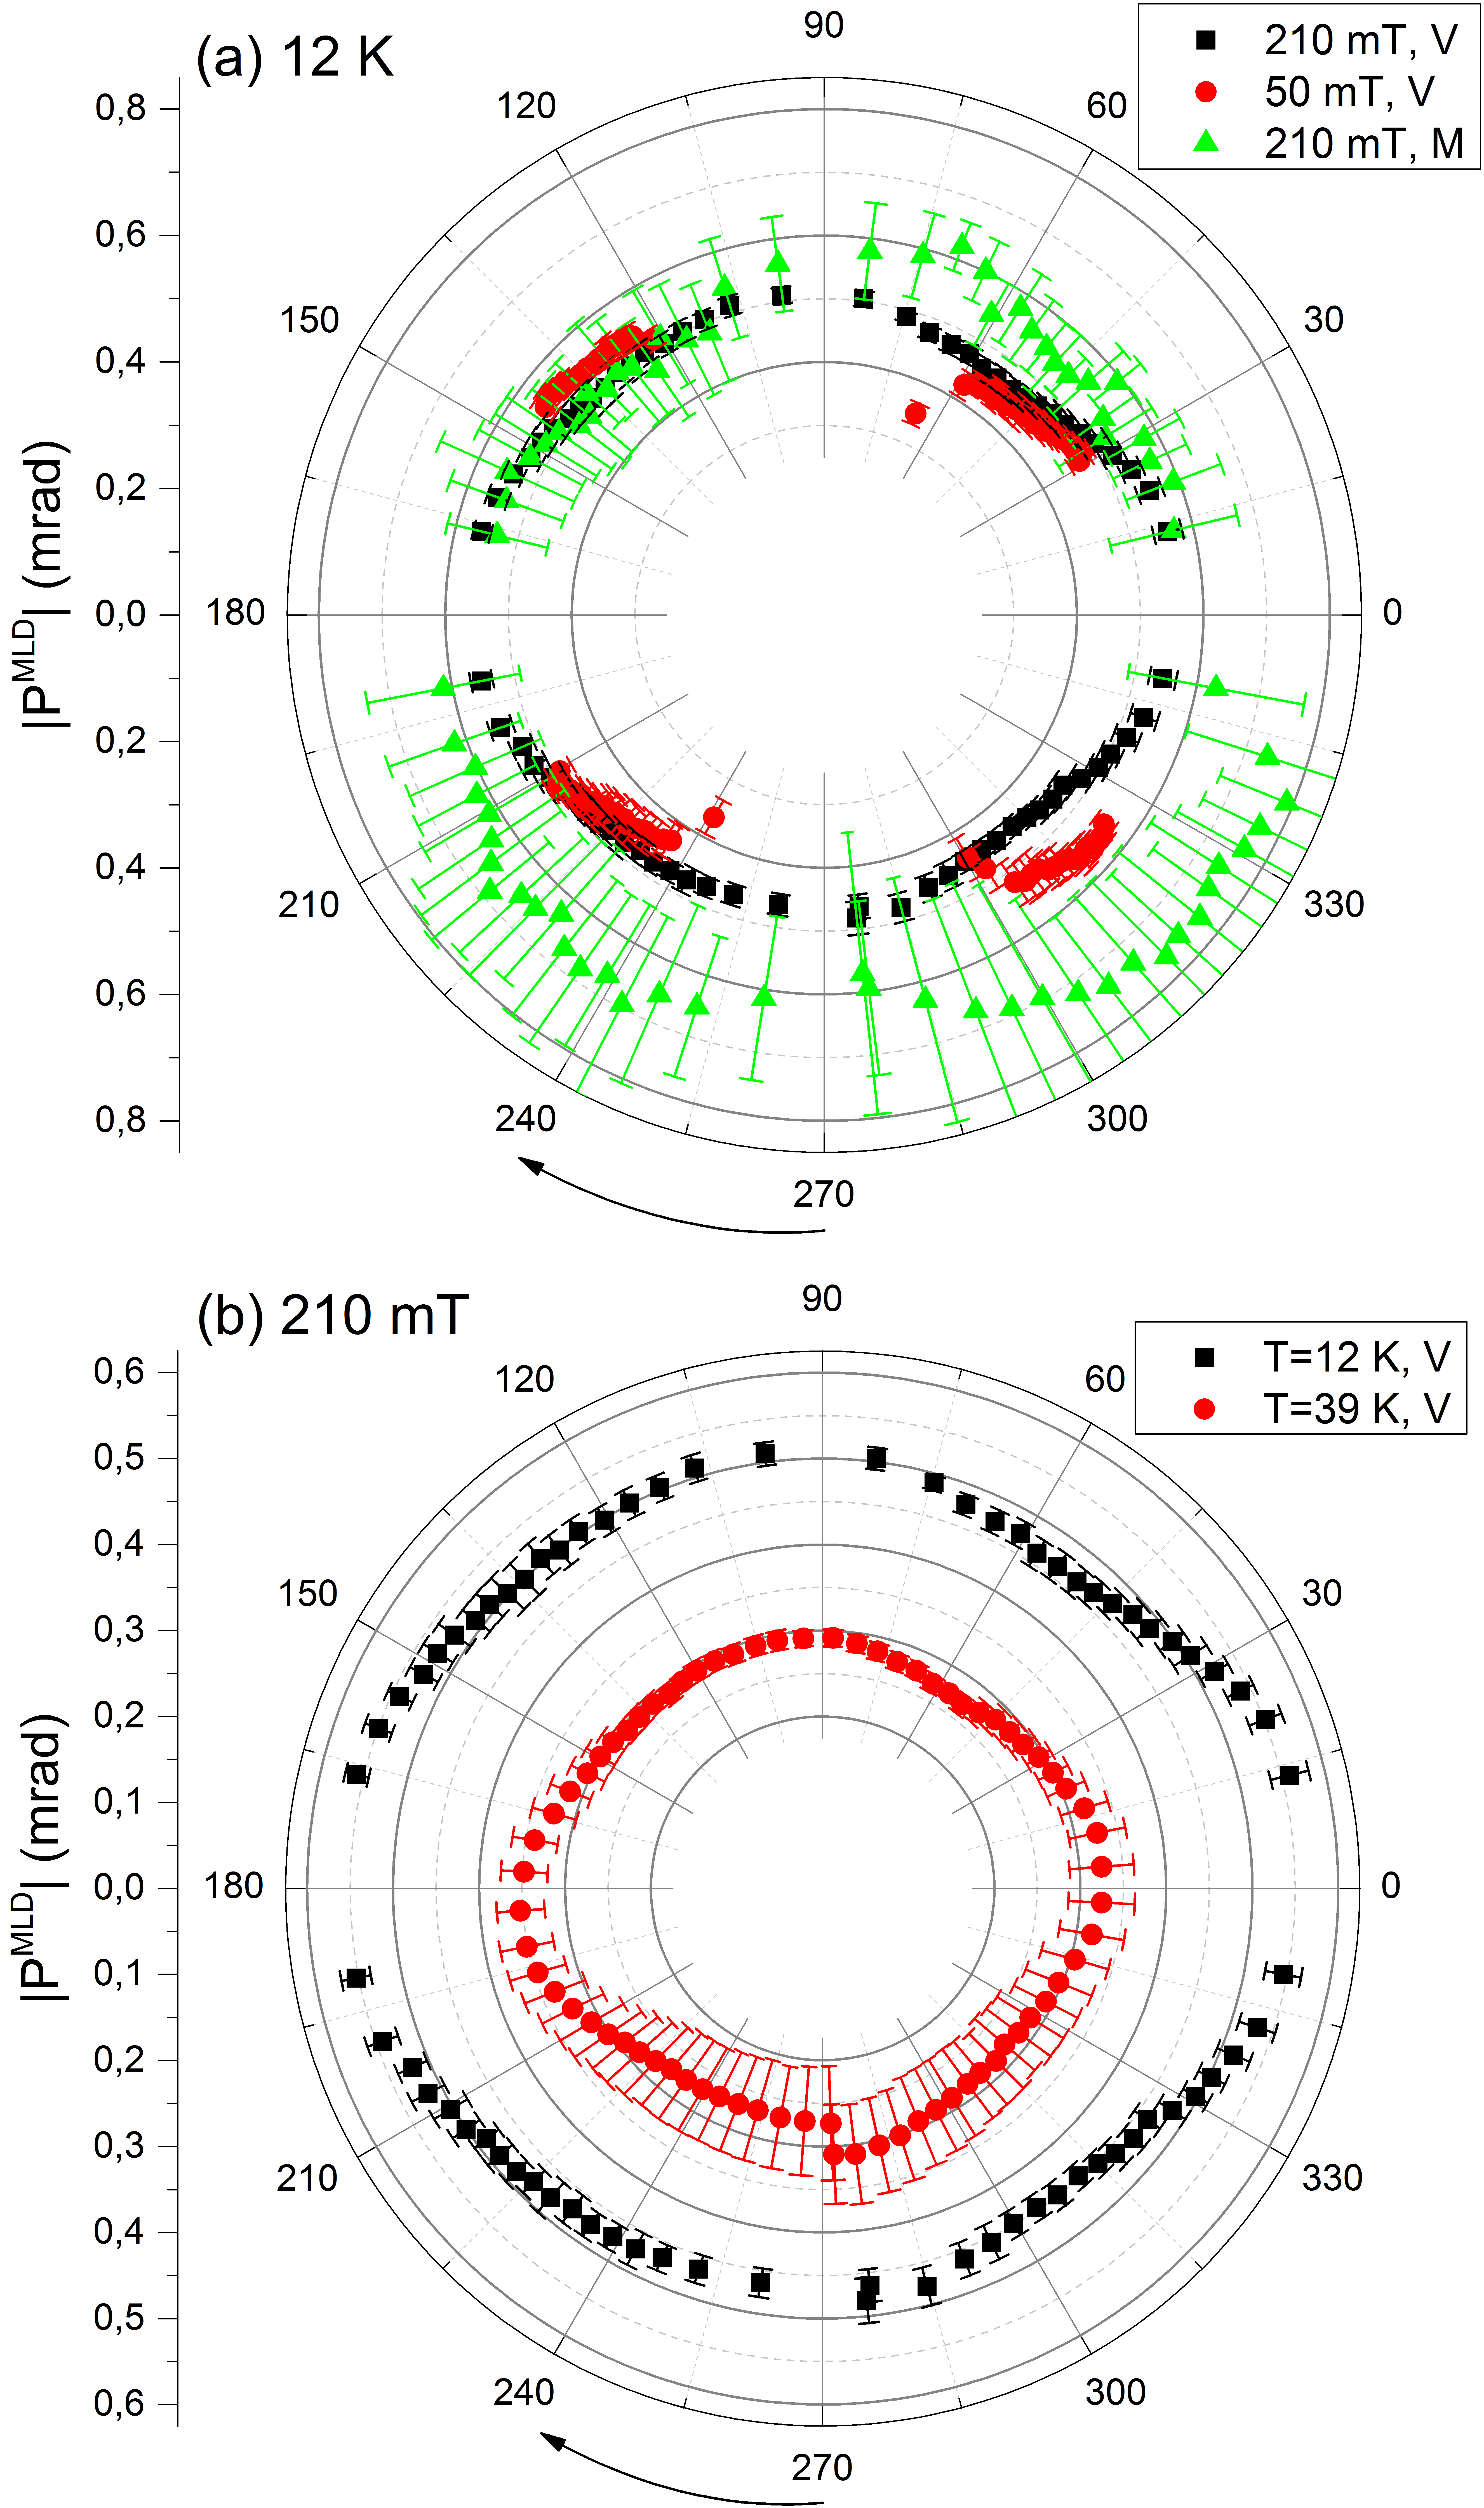
\includegraphics[width=0.8\textwidth]{./png/tocgraf_pmldvse}}
	\caption{Změna směru pole při jeho konstantní velikosti. Závislost nafitované $\pmld$ na směru magnetizace $\phM$ (viz. obr \ref{toc_vysledkyuhel}). $\pmld$ je záporné, v~grafu je vynesena absolutní hodnota. (a) Dvě různé velikosti pole $\hext$ při $T<\SI{15}{\kelvin}$. (b) $\mu_0\hext=\SI{210}{\milli\tesla}$ při dvou různých teplotách $T=\SI{12(3)}{\kelvin}$ a \SI{38,7(10)}{\kelvin}. V -- Voigtův jev, M -- MLD.}\label{toc_vysledkypmld}
\end{figure}
\chapter*{Závěr}
\addcontentsline{toc}{chapter}{Závěr}

V práci jsme se věnovali studiu magnetooptických jevů v dobře prostudovaném vzorku feromagnetického polovodiče GaMnAs pomocí nově postaveného prototypu 2D elektromagnetu.

Nejprve jsme ověřili použitelnost elektromagnetu přesným zopakováním experimentů provedených v práci \cite{Reichlova} s jiným elektromagnetem. Jednalo se o měření Voigtova jevu a MLD v hysterezních smyčkách. Poté jsme vyzkoušeli novou variantu experimentálního uspořádání, které nám umožňuje kolmý dopad světla na vzorek. Nakonec jsme vyzkoušeli novou metodu, ve které při konstantní velikosti vnějšího pole měníme jeho směr.
Naše měření jasně ukázala, že pomocí Voigtova jevu a MLD je možné velice efektivně určit magnetickou anizotropii vzorku (konkrétně určit polohu snadných os magnetizace). Měření využívající změnu směru konstantního magnetického pole dále umožňuje od sebe oddělit na krystalografickém směru závislé a nezávislé složky příslušného magnetooptického koeficientu.


%%% Seznam použité literatury
%%% Seznam použité literatury (bibliografie)
%%%
%%% Pro vytváření bibliografie používáme bibTeX. Ten zpracovává
%%% citace v textu (např. makro \cite{...}) a vyhledává k nim literaturu
%%% v souboru literatura.bib.
%%%
%%% Příkaz \bibliographystyle určuje, jakým stylem budou citovány odkazy
%%% v textu. V závorce je název zvoleného souboru .bst. Styly plainnat
%%% a unsrt jsou standardní součástí latexových distribucí. Styl czplainnat
%%% je dodáván s touto šablonou a bibTeX ho hledá v aktuálním adresáři.

\bibliographystyle{unsrt}    %% Autor (rok) s českými spojkami
% \bibliographystyle{plainnat}    %% Autor (rok) s anglickými spojkami
% \bibliographystyle{unsrt}       %% [číslo]

\renewcommand{\bibname}{Seznam použité literatury}

%%% Vytvoření seznamu literatury. Pozor, pokud jste necitovali ani jednu
%%% položku, seznam se automaticky vynechá.

\bibliography{literatura}

%%% Kdybyste chtěli bibliografii vytvářet ručně (bez bibTeXu), lze to udělat
%%% následovně. V takovém případě se řiďte normou ISO 690 a zvyklostmi v oboru.

% \begin{thebibliography}{99}
%
% \bibitem{lamport94}
%   {\sc Lamport,} Leslie.
%   \emph{\LaTeX: A Document Preparation System}.
%   2. vydání.
%   Massachusetts: Addison Wesley, 1994.
%   ISBN 0-201-52983-1.
%
% \end{thebibliography}




%%% Použité zkratky v bakalářské práci (opět nemusí být nutné uvádět)
%%% U matematických prací může být lepší přemístit seznam zkratek na začátek práce.

%%% Přílohy k bakalářské práci, existují-li. Každá příloha musí být alespoň jednou
%%% odkazována z vlastního textu práce. Přílohy se číslují.
%%%
%%% Do tištěné verze se spíše hodí přílohy, které lze číst a prohlížet (dodatečné
%%% tabulky a grafy, různé textové doplňky, ukázky výstupů z počítačových programů,
%%% apod.). Do elektronické verze se hodí přílohy, které budou spíše používány
%%% v elektronické podobě než čteny (zdrojové kódy programů, datové soubory,
%%% interaktivní grafy apod.). Elektronické přílohy se nahrávají do SISu a lze
%%% je také do práce vložit na CD/DVD. Povolené formáty souborů specifikuje
%%% opatření rektora č. 72/2017.
\appendix
\chapter{Přílohy}

\section{Odvození polarizační závislosti MLD} \label{odvozeni_mld}
Na vzorek kolmo dopadá světlo s intenzitou $I_0$ lineárně polarizované ve směru $\beta$. Magnetizace je v rovině vzorku pod úhlem $\phM$ a koeficienty reflexe pro polarizaci rovnoběžnou, resp. kolmou na magnetizaci jsou $r_\paral$, $r_\perpen$.

Intenzita je úměrná čtverci $\vec{E}$
\begin{equation}
I_0 \propto E^2 \,,
\end{equation}
stejně odražená intenzita $I^\prime$ je úměrná čtverci odražené $\vec{E^\prime}$
\begin{equation}
\begin{aligned}
I^\prime \propto {E^\prime_\paral}^2 + {E^\prime_\perpen}^2 &= ({r_\paral E \cos(\phM-\beta)})^2+({r_\perpen E \sin(\phM-\beta)})^2 \\
&=E^2 \left[r_\paral^2 \cos^2(\phM-\beta)+ r_\perpen^2 \sin^2(\phM-\beta)\right] \\
&=E^2 \left[ \frac{r_\paral^2+r_\perpen^2}{2}  +  \left( \frac{r_\paral^2}{2} - \frac{r_\perpen^2}{2}\right) \cos[2(\phM-\beta)]\right] \\
&=E^2 \frac{r_\paral^2+r_\perpen^2}{2} \left[1 + 2\pmld \cos[2(\phM-\beta)]\right]
\end{aligned}
\end{equation}
a tedy
\begin{equation}
I^\prime=I_0 R \left[1 + 2\pmld \cos[2(\phM-\beta)]\right] \,,
\end{equation}
kde jsme označili $R=(r_\paral^2+r_\perpen^2)/2$ a použili přiblížení $r_\paral /r_\perpen \approx 1$, ve kterém platí $\pmld =\num{0,5}(r_\paral^2-r_\perpen^2)/(r_\paral^2+r_\perpen^2)$.

Zavedeme veličinu $B:=I^\prime/(I_0R)-1$. Potom
\begin{equation}
B=2\pmld \cos[2(\phM-\beta)] \,.
\end{equation}

Při měření hysterezních smyček bude mít intenzita podobný průběh jako v~případě Voigtova jevu. Při přeskoku mezi snadnými osami dojde ke skoku v intenzitě, který bude mít amplitudu $\Delta B=B_4-B_1$.
\begin{equation}
\Delta B=2 \pmld \left( \cos[2({\phM}_4-\beta)] -\cos[2({\phM}_4-\beta)] \right) \,,
\end{equation}
kde ${\phM}_1$ a ${\phM}_2$ jsou směry snadných os, mezi kterými došlo k přeskoku magnetizace. Při stejném označení úhlů jako v \ref{revsci_mld} (d) platí
\begin{equation}
\begin{aligned}
\Delta B &=2 \pmld \left( \cos\left[2\left(\gamma+\frac{\xi}{2}-\beta\right)\right] -\cos\left[2\left(\gamma-\frac{\xi}{2}-\beta\right)\right] \right) \\
&=-4\pmld  \sin[2(\gamma-\beta)]\sin(\xi) \,.
\end{aligned}
\end{equation}
\section{Odvození korekcí v kolineární geometrii}
\label{odvozeni_kolinearni}

V kolineární geometrii jsme od sebe nedokázali oddělit svazek odražený od vzorku a svazek odražený od okénka kryostatu, což nám do měřených napětí zanáší parazitní signál. Získání magnetooptických signálů $\Delta\beta$ a $B$ pak vyžaduje korekci.

Předpokládáme, že polarizační stav světla odraženého od sklíčka je nezávislý na vnějším magnetickém poli. Na sklíčko dopadá intenzita $I_0$. Označíme $R_S=\SI{4}{\percent}$ intenzitní odrazivost sklíčka a $R_V=\SI{33}{\percent}$ intenzitní odrazivost vzorku.
Světlo odražené od sklíčka má intenzitu (odraz od přední a zadní strany sklíčka, další odrazy jsou zanedbatelné)
\begin{equation}
I^S=(R_S+R_S(1-R_S)^2) I_0:=\rho_S I_0
\end{equation}
a světlo odražené od vzorku má intenzitu (odraz od vzorku a čtyřnásobný průchod rozhraní sklíčka)
\begin{equation}
I^V=(1-R_S)^4 R_V I_0 := \rho_V I_0 \,.
\end{equation}
Celková intenzita je dána jejich součtem. Spočteme, čemu se rovná výraz, kterým jsme v nekolineární geometrii počítali $\Delta\beta$
\begin{equation}
\begin{aligned}
\frac{I_A-I_B}{2(I_A+I_B)}&=\frac{I^S_A-I^S_B}{2I}+\frac{I^V_A-I^V_B}{2(I^V_A+I^V_B)}\frac{I^V}{I^S+I^V} \\
&=\text{konst}+\Delta\beta \frac{\rho_V}{\rho_S+\rho_V} \,.
\end{aligned}
\end{equation}
První člen je konstanta vzhledem k vnějšímu magnetickému poli ($I$ se sice vlivem MLD mění, tento vliv je však zanedbatelný při $r_\paral/r_\perpen\approx 1$), které se zbavíme vyvážením můstku.
$\Delta\beta$ tedy získáme stejně jako v nekolineární geometrii, pouze navíc vynásobíme konstantou
\begin{equation}
\frac{\rho_S+\rho_V}{\rho_V}\approx \num{1,27} \,.
\end{equation}

Pro celkovou intenzitu platí
\begin{equation}
I=I_S+I_V=I_0\rho_S+I_0\rho_V(1+B)=I_0(\rho_S+\rho_V)\left(1+B\frac{\rho_V}{\rho_S+\rho_V}\right) \,.
\end{equation}
Pokud součtový signál zpracujeme stejným způsobem jako v nekolineární geometrii, pak opět vynásobením $(\rho_S+\rho_V)/\rho_V$ obdržíme už správnou hodnotu $B$.

Zpracování hrubých dat je v kolineární geometrii totožné jako nekolineární, pouze konečné veličiny $\Delta\beta$ a $B$ vynásobíme číslem \num{1,27}.

\openright
\end{document}
